% History
%  04/29/08  jcv few more final mods
%  01/27/08  jcv some modifications and simplifying
%  05/15/06  kg made available to UMD Astro Wiki
%  01/12/05  kg retrieved from DSR 
%  05/27/04  DSR  retrieved from Wayne Baumgartner
%

% Official version for University
% Also, do not use \makecover for official version.
\documentclass[12pt,letterpaper,oneside]{dissertation}

% Use the following instead of the above for duplex printing.
%  Makes ``inside'' margins 1.5 inches.  Also forces odd-numbered
%  pages to be on the right, and forces new chapters to be on
%  odd-numbered pages
%\documentclass[12pt,letterpaper,twoside]{dissertation}

%jam added this to get glossaries to work
% arara: pdflatex
% arara: bibtex
% arara: makeglossaries
% arara: pdflatex    
%% arara: pdflatex  
\usepackage{longtable} 
\usepackage{subfigure}
\usepackage{graphicx}
\usepackage{ifthen}
\usepackage{epstopdf}
% To use AAS macros
\usepackage{sty/aastex_hack}
% Use improved verbatim package for included code and force single
% spacing in it.
\usepackage{fancyvrb}
\fvset{baselinestretch=1}
% Package to deal with acronyms nicely
\usepackage{acronym} %jam maybe comment this out?
%Jam added glossaries
%Jame trying to get deluxetable to play nice with glossaries which includes supertabular

%jam added lineno, not sure we need it?
\usepackage{lineno}
%\linenumbers

\usepackage[nomain,acronym,toc, nonumberlist]{glossaries}
\let\shead = \tablehead
\let\stail = \tabletail
\let\tablehead\relax
\let\tabletail\relax
\let\tablecaption\relax
\usepackage{sty/deluxetable}
\let\thead=\tablehead
\let\ttail=\tabletail
\let\tcap=\tablecaption
\let\tablehead =\thead
\let\tabletail =\ttail
\let\tablecaption =\tcap

\renewcommand*{\acronymname}{List of Symbols and Acronyms}
\loadglsentries{abbrev}
%%List of abbreviations
%\newaonym[longplural={Frames per Second}]{fpsLabel}{FPS}{Frame per Second}

%\newacronym{LAT}{name = {LAT}, text ={lare area telescope}, description ={ Large Area Telescope}}%simple example
%\newglossaryentry{uppercase}{
%	name={Uppercase},
%	text={uppercase},
%	description={Appears uppercase in the glossary and lowercase in the text}
%}

\newacronym{onefgl}{1FGL}{First \emph{Fermi}-LAT source catalog}
\newacronym{twofgl}{2FGL}{Second \emph{Fermi}-LAT source catalog}
\newacronym{threefgl}{3FGL}{Third \emph{Fermi}-LAT source catalog}
\newacronym{onefhl}{1FHL}{First Catalog of Hard \emph{Fermi}-LAT Sources}
\newacronym{twofhl}{2FHL}{Second Catalog of Hard \emph{Fermi}-LAT Sources}
\newacronym{twopc}{2PC}{Second \emph{Fermi}-LAT catalog of Gamma-ray Pulsars}
\newacronym{acd}{ACD}{anti-coincidence detector}
\newacronym{agn}{AGN}{active galactic nuclei}
\newacronym{bpl}{BPL}{broken power law}
\newacronym{calo}{CAL}{Calorimeter}
\newacronym{cmb}{CMB}{Cosmic Microwave Background}
\newacronym{cgro}{CGRO}{Compton Gamma-Ray Observatory}
\newacronym[plural=CRs]{cr}{CR}{cosmic ray}
\newacronym{cta}{CTA}{Cherenkov Telescope Array}
\newacronym{dsa}{DSA}{diffusive shock acceleration}
\newacronym{dm}{DM}{dispersion measure}
\newacronym{ecpl}{ECPL}{exponentially cut-off power law}
\newacronym{egret}{EGRET}{Energetic Gamma-Ray Experiment Telescope}
\newacronym{fov}{FoV}{field of view}
\newacronym{fir}{FIR}{far infrared}
\newacronym{gbm}{GBM}{Gamma-Ray Burst Monitor}
\newacronym{grb}{GRB}{gamma-ray burst}
\newacronym{he}{HE}{high energy}
\newacronym{hep}{HEP}{highest-energy photon}
\newacronym{hess}{H.E.S.S.}{the High Energy Stereoscopic System}
\newacronym{ic}{IC}{inverse Compton}
\newacronym{iem}{IEM}{interstellar emission model}
\newacronym{irf}{IRFs}{instrument response functions}
\newacronym[plural=IACTs]{iact}{IACT}{Imaging Air Cherenkov Telescopes}
\newacronym{ism}{ISM}{interstellar medium}
\newacronym{lat}{LAT}{Large Area Telescope}
\newacronym{lrt}{LRT}{likelihood ratio test}
\newacronym{magic}{MAGIC}{the Major Atmospheric Gamma-ray Imaging Cherenkov telescopes}
\newacronym[plural =MCs]{mc}{MC}{molecular cloud}
\newacronym{msp}{MSP}{millisecond pulsar}
\newacronym{nir}{NIR}{near infrared}
\newacronym{ns}{NS}{neutron star}
\newacronym{pl}{PL}{power law}
\newacronym{psf}{PSF}{point spread function}
\newacronym[plural=PSRs ]{psr}{PSR}{pulsar}
\newacronym[plural=PWNe ]{pwn}{PWN}{pulsar wind nebula}
\newacronym[plural=RoIs ]{roi}{RoI}{region of interest}
\newacronym[plural=SEDs]{sed}{SED}{spectral energy distribution}
\newacronym{sedt}{ST}{Sedov-Taylor}
\newacronym[plural=SNRs ]{snr}{SNR}{supernova remnant}
\newacronym{tkr}{TKR}{tracker}
\newacronym{ts}{TS}{test statistic}
\newacronym{veritas}{VERITAS}{the Very Energetic Radiation Imaging Telescope Array System}
\newacronym{vhe}{VHE}{very high energy}
\newacronym{snrmc}{SNR-MC}{supernova remant molecular cloud system}



%So I don't have to type gls all the time

%List of Symbols

\newglossaryentry{nh}
{
	name={\ensuremath{~\mathrm{N_{\rm{H}}}}},
	description={Neutral Hydrogen Number Density},
	sort=Nh
}

\makeglossaries
%jam not sure I need an index
%\usepackage[xindy]{imakeidx}
%\makeindex

% Instruction to natbib package to omit comma between name and date
% within citations as well as to do name-date citation style the sort
% option forces output of multiple items to be in the order that they
% show up in Bibliography.
\usepackage[authoryear,round,sort]{natbib}
\bibpunct{(}{)}{;}{a}{}{,}
\usepackage{sty/natbibspacing}

% Where I define my personal macros; probably should input this instead
\usepackage{sty/mydefs}

% To fiddle with captions
\usepackage[small]{caption}
% Instruction to caption.sty to make a 20pt margin on each side of
% captions
\setlength{\captionmargin}{20pt}
% To single space captions, tables, etc.
\usepackage{sty/atbeginend}

% To reduce the size of chapter, etc headings
\usepackage{sectsty}
\chapterfont{\huge\centering}
\usepackage[nobottomtitles]{titlesec}

\usepackage{pdfpages}
\usepackage{hyperref}
\hypersetup{
pdfauthor = {Jamie Michael Cohen},
pdftitle = {Doctor of Philosophy, 2016},
pdfsubject = {Subject Dissertation},
}
% Depth of section numbering in body 
%\setcounter{secnumdepth}{3}

% Fix spacing in floats
% atbeginend.sty stuff: (spacing commands defined in dissertation.sty)
\BeforeBegin{deluxetable}{\spacing{1}}
\AfterEnd{deluxetable}{\spacing{\bodyspacing}}
\BeforeBegin{table}{\spacing{1.1}}
\AfterEnd{table}{\spacing{\bodyspacing}}
\BeforeBegin{figure}{\spacing{1.1}}
\AfterEnd{figure}{\spacing{\bodyspacing}}
\BeforeBegin{figure*}{\spacing{1.1}}
\AfterEnd{figure*}{\spacing{\bodyspacing}}

% For intelligent float placement fiddle with these
\renewcommand{\topfraction}{0.9}
\renewcommand{\bottomfraction}{0.9}
\renewcommand{\floatpagefraction}{0.75}
\renewcommand{\textfraction}{0.1}
\renewcommand{\dbltopfraction}{0.75}

% Make the front matter 
% Long titles need to have breaks forced within them with \\ at break.
\title{\g-Ray Studies of Stellar Graveyards: \\ Observations of Extended Emission from \\
	 Supernova Remnants and Pulsar Wind Nebulae.}

\author{Jamie Michael Cohen} % You should really have full name here.
\date{2016} % Date of your degree.
\department{Astroparticle Physics Laboratory, Code 661 \\ NASA Goddard Space Flight Center}
\advisor{Doctor Elizabeth Hays}
\chairtitle{Chair/Advisor}
\advtitle{Advisor}
\chairdept{Department of Astronomy \\ University of Maryland}
\chairname{Professor M. Coleman Miller}
% Rest of committee in alphabetical order with title.  Any type of
% professor (assistant, associate, or adjunct) gets ``Professor.''
\committee{Professor Christopher S. Reynolds \\
                Professor Derek C. Richardson \\
                Doctor Who}

% Comment out the following three lines if you don't want to dedicate
% your thesis, you uninspired piece of scum.
\phantomsection
\label{mydedication}
\dedication{\centering To Vanessa!}

% Abstract is required for UMD as of 2006.
\abstractfile{abstract}

% Just comment out if you don't want to acknowledge anyone, you
% ungrateful little pipsqueak.
\acknowledgements{I should probably thank someone because I'm not a degenerate.
}

% Just comment out if you don't want to ace your work.
\prefacefile{preface}

% If you can't figure out what the following are for, you shouldn't be
% getting a PhD.
\setboolean{hasfigures}{true}
\setboolean{hastables}{true}
\setboolean{hascopyright}{true}

\begin{document}
%\makecover adds a file cover.pdf to the front for UNOFFICIAL Version
%only.
%\makecover
\makefrontmatter

%%%%%%%%%%%%%%%%%%%%%%%%%%%%%%%%%%%%%%%%%%%%%%%%%%%%%%%%%%%%%%%%%%%%%%%%%%%
% CHAPTERS one include for each
\chapter{Overview}
\label{chap:intro}

\begin{quote}
	``Maybe I'll have a super relevant quote here!'' 
	\begin{center}---by some awesome human, from \it{Some book} \end{center}
\end{quote}
%\begin{figure*}
%  \centering
%  \epsscale{1}
  % Jamie commented this out for now
 % \plotone{figures/filename-with-no-extension}
%  \caption[Short Caption]{Long caption}
%  \label{fig:somelabel}
%\end{figure*}

\section{Goooo $\gamma$-rays go!}
\jamie{Maybe I should just move the gamma-ray astro, LAT, and SNR chapters here and have them all be  sections in the intro. Or maybe, This section is a super short overview of the entire thesis, next section is all the bkg.}
In this thesis we...or should I start with the extreme environs line?

Overview of the entire thesis, why gamma-rays, why the \lat, why \snr and \pwn and extended sources.

Higher energy studies with the LAT have been my focus since the beginning. Talk about what's nice about staying above 1 GeV, 10 GeV, 50 GeV. 

GeV TeV connection for 2FHL

Radio GeV for SNR cat (traces same particle population)

The advent of the \lat presents for the first time the capability to spectrally and spatially resolve \gls{snr} at \gev energies.

it is uniquely situated to address these issues

egret was mostly pointed observation instrumented that would sometimes dwell on a spot for a couple of weeks, had a smaller field o view, didn't get as many photons (the LAT saw the entire EGRET sky in some short amount of time)

\snrs as sources of relativistic particles

Despite being the prime energy range to observe the effects of cosmic particle acceleration, the photon \sed{} resulting from these overlapping emission channels are often difficult to spectrally distinguish from one another. \jamie{what's the point of this last sentence here? maybe no need to mention this now, i really just want to motivate GeV energies}

when talking about \egret{}

With its unprecedented sensitivity and angular resolution above 1\gev, the \lat~provides for the first time the opportunity to distinguish SNR-emitted photons from their backgrounds, and  to unambiguously detect and identify dozens of \glspl{snr}. \jamie{maybe this is for the intro/abstract because it's a little vague}

The \lat{} is uniquely situated to address these goals and definitively detect and identify dozens \snrs

snrs as source of Galactic cosmic rays, and thus as drivers of Galactic evolution

\cite{Thomson93} gives the 68\% containment radius as $\theta \leq 5.85^\circ (E_\gamma /100 \mev )^{-0.534}$
\section{I Think I Hate Most of the Section Titles :(}

\section{Maybe None of the Chapters Need Introductions?}

\section{Dissertation Overview}




\chapter{Gamma-ray Astronomy }
\label{chap:gamAstr}

\section{Introduction}\label{gamAstr:intro}
Maybe this is not just gamma astro, but gamma astro of SNRS

The story of \gam 's from astrophysical objects is a tale of the most extreme, energetic, and violent environments in our universe. Discovered by Paul Villard studying radiation from radium and named by Ernest Rutherford, who previously uncovered the nature of $\alpha$ and $\beta$ radiation, \gam's are the highest named energy of light 

more historical context instead of a separate section


what is a gamma-ray

why bother studying gamma-rays

probe of extreme environments



\section{\gam~Emission Mechanisms }\label{gamAstr:CR}
Gamma-rays as a probe of cosmic rays and cosmic acceleration processes

gamma-ray astronomy as  a proxy for studying cosmic rays and acceleration/diffusion processes. How much to get into CR. 

Cosmic particle accelerators and \gam's
accelerator plus target often 


What's a CR, quick,  general CR properties that are relevant to SNRs

why use gamma's  to study CR

gamma-ray production mechanisms

-Synch,
-Bremss,
-IC,
-pi0,

\section{Sources of \gam's}\label{gamAstr:Sources}
Maybe don't need this? The reason to is to say SNRs early on. Would I mention other sources to be complete?

SNRs as the primary source of Galactic CRs, order of mag (zwicky?) energy from 0.1*E SNR could account for energy in CRs in Galaxy

\section{\gam~Detection}\label{gamAstr:Detect}
Quick rehash of method of detecting \gam's? Or is this just about previous \gam ~detectors and the state of the \gam~sky pre-Fermi?  mention telescopes up to EGRET, bit of detail on EGRET and what the pre-Fermi \gam~sky looked like, in particular in the context of SNRs, PWN, Galactic plane

gamma-ray telescopes leads into the LAT, Egret was  predecessor , what it did and what were some relevant unanswered questions regarding supernova remnants 

\citep{Esposito96}
\citep{Sturner95}

\section{Scratch}


Altho' many miles from bomb zero, Dr. Bruce Banner is bathed in the full force of the mysterious Gamma Rays!

\chapter{The \Fermi ~Gamma-Ray Space Telescope and \gam ~Data Analysis}
\label{chap:FGST}

\section{\label{FGST:intro}Introduction}
The \Fermi~Gamma-Ray Space Telescope (\Fermi ~hereafter), successor to the \egret~instrument on \cgro, was successfully launched into orbit around Earth on June 11 2008. \Fermi ~consists of two instruments, the LAT and the \gbm.

The LAT, which is the primary instrument on \Fermi, is a pair conversion telescope designed to detect photons from 20 \mev~to greater than 1 \tev. Its standard mode of operation is a sky-survey mode in which it observes the entire sky every 3 hours. The \gbm~is designed to detect \glspl{grb} in a waveband overlapping that of the \lat,  and complementary in lowering that energy range.  It is comprised of two types of scintillator detectors: two bismuth germanate crystals that operate from 150 \kev~ to 30 \mev, and 12 sodium iodide crystals sensitive to photons  between 8 \kev~and 1 \mev. 

Combined the \lat~and \gbm~ make up a formidable observatory, spanning more than 8 decades in energy, and is  currently the only instrument performing all-sky observation in this broad energy range.  \jamie{maybe I don't need any gbm stuff? I mentioned it just to be complete about what fermi is, probably won't mention it again, and this last par doesn't really flow into the next }


\section{\label{FGST:LAT}The Large Area Telescope}
The need for Fermi in the context of what EGRET did

What were open questions from EGRET era, state of \gam~detection of SNRs, what question was Fermi deigned to answe

Description of the instrument
 \jamie{not sure this really goes here, separate section for what questions  Fermi was designed to answer?}
 
 
 track and reconstruct the path of 
 Describe it's objectives and strengths over predecessors
 Details on the LAT and it's design, be sure to focus on things that particularly pertinent to the work I've done like what determines the PSF, thing about Pass 8 here maybe? Or maybe later on. 
 
 what science was it designed to answer
 
 general capabilities
 
 details about aspect of the LAT related to extended sources, what determines PSF
 \section{\label{FGST:analysis}\gam~Data Analysis}
 
 Why maximum likelihood, how it's formulated,  implemented in the Science Tools, pointlike and the analysis for extended sources. Diffuse emission.
 
 
 Four steps to going from observing the sky to final LAT analysis:
 
 Instrument taking data: How we get to counts
 
 Reconstruction : How we get photons
 
 Likelihood: How to characterize sky using response functions, point source  and diffuse modeling
 
 Likelihood for ES: how to use likelihood methods to char and resolve sources measure  extension
 
 Section on diffuse emission
\subsection{\label{FGST:sub}Do I need subsections?}
\section{Scratch}
\psf



I'm not sure about this chapter yet. Maybe it's a general section on Analysis of Fermi data,



%\chapter{Analysis of \lat- data}
\label{chap:fermiData}
I'm not sure about this chapter yet. Maybe it's a general section on Analysis of Fermi data, why maximum likelihood, how it's formulated,  implemented in the Science Tools, pointlike and the analysis for extended sources. Diffuse emission

Four steps to going from observing the sky to final LAT analysis:

Instrument taking data: How we get to counts

Reconstruction : How we get photons

Likelihood: How to characterize sky using response functions, point source  and diffuse modeling

Likelihood for ES: how to use likelihood methods to char and resolve sources measure  extension


\section{addSrcs}

 %merged with LAT section
\chapter{Supernova Remnants: Theory and  Observation}
\label{chap:Rems}

\section{Introduction}\label{Rems:intro}
Why study SNRs, what they are, history of SNR,  radio detections, 



\section{\label{Rems:evo}Formation and Evolution}

-Stars die and explode, that energy is very quickly put into the surroundings
    
-snowplough, ST, radiative,
    
- what else?

How we detect gamma-rays from SNRs/PWNe in the Galaxy leads to and analysis section maybe?
\section{\label{Rems:obs}Morphology and Classification}

SNRs characterized by morphology and evolution properties

shell type, mixed morphology, filled center  composite )

Since I eventually do these all plane surveys, what does the spatial  distribution of them at radio look like?

Not sure how much to say about radio observations, x-ray, TeV

\section{\label{Rems:CR}Cosmic Ray SNR connection}

Give the whole, if 10\% of energy of SN explosion goes into particle acceleration, we can explain cosmic rays

Particle acceleration and DSA

This leads to gamma-ray section

	
\section{Summary}\label{Rems:summ} In this section we summarized the end phase of stellar evolution (just enough to motivate SNRs) and descried the environs surrounding the supernova; development and phases of \glspl{snr} (and \glspl{pwn}?).  In particular we detailed the nonthermal emission mechanisms that produce \g-ray radiation, detection of young vs middle-aged( evolved, interacting with surroundings/dense medium),TeV detects younger typically, the troubles of detecting extension from them(?) something about different emission zones? Troubles disentangling hadronic from leptonic at \g-rays. \g-ray spectral and morphological features. Trends across the population wrt spectral shape/breaks, higher luminosity for interacting rems. Cosmic rays, using gamma-rays to probe CR population. So much of \g-ray astro is really about studying CRs, how much to say about them? 

\section{Scratch}
This chapter needs a different title. It's more focused on the specific sources being studied in this thesis. Galactic extended sources, SNRs, PWNe, but as in the SNRcat, not just extended SNRs, point-like SNRs as well.

Less focus on PWNe. Only give as much as I feel I need to support mentioning them a bit for 2FHL?

The focus of this section is supernova remnants in a gamma-ray context. Theory of evolution, what the gamma-ray emission is like, what we can learn from them individually.  This leads to the 1st SNR cat section for what we can do with them ensemble

NOt sure I really need any PWN stuff yet

in 2FHL we detect some pwn. If including above 10gev work, they'll be there too. Much of the thesis is really about extended gamma-ray sources, but not sure how that fits into the title and chapters yet

Do I need to get into composite SNRs (composite means SNR + PWN ) Maybe relevant for G150? Some things about interaction of reverse shock with PWN and crushing/reverberations of the PWN?

\cite{Montmerle79}
\chapter{Revealing the GeV Supernova Remnant Population}
\label{chap:snrCat}


%\section{Introduction}\label{snrCat:Intro}
\section{\label{snrCat:latGam}Supernova Remnants at \gam~Energies}

By the end of the its science run, \egret{} had detected 271 sources above 100\mev{}, within a minimum detection significance of 4$\sigma$, 170 of which had no clear multiwavelength counterpart, with 81 of those unidentified lying within \blat of the Galactic plane \citep{Hartman99}. The main hindrances to source identification were the numerous potential source counterparts (the \egret{} \psf{} was energy dependent, with a 68\% containment radius of ${\rm \sim 6 ^\circ}$ at 100\mev{} and smaller for higher energies) and the large \egret{} error boxes. In addition to this, the primary method for identifying a \gam{} source as an \snr{} is through a compatible angular extent with  observations at some other wavelength, thus the ability to resolve emission from an \snr{} is vital to understanding the mechanisms therein giving rise to \gam{}s. Figure \ref{fig:3EGSky} shows an \egret{} all-sky map at ${\rm E > 100 \mev}$ where the preponderance of unidentified sources and locations thereof are made clear.  


\begin{figure}[h!]%[t] 
	\centering
	\makebox[\linewidth]{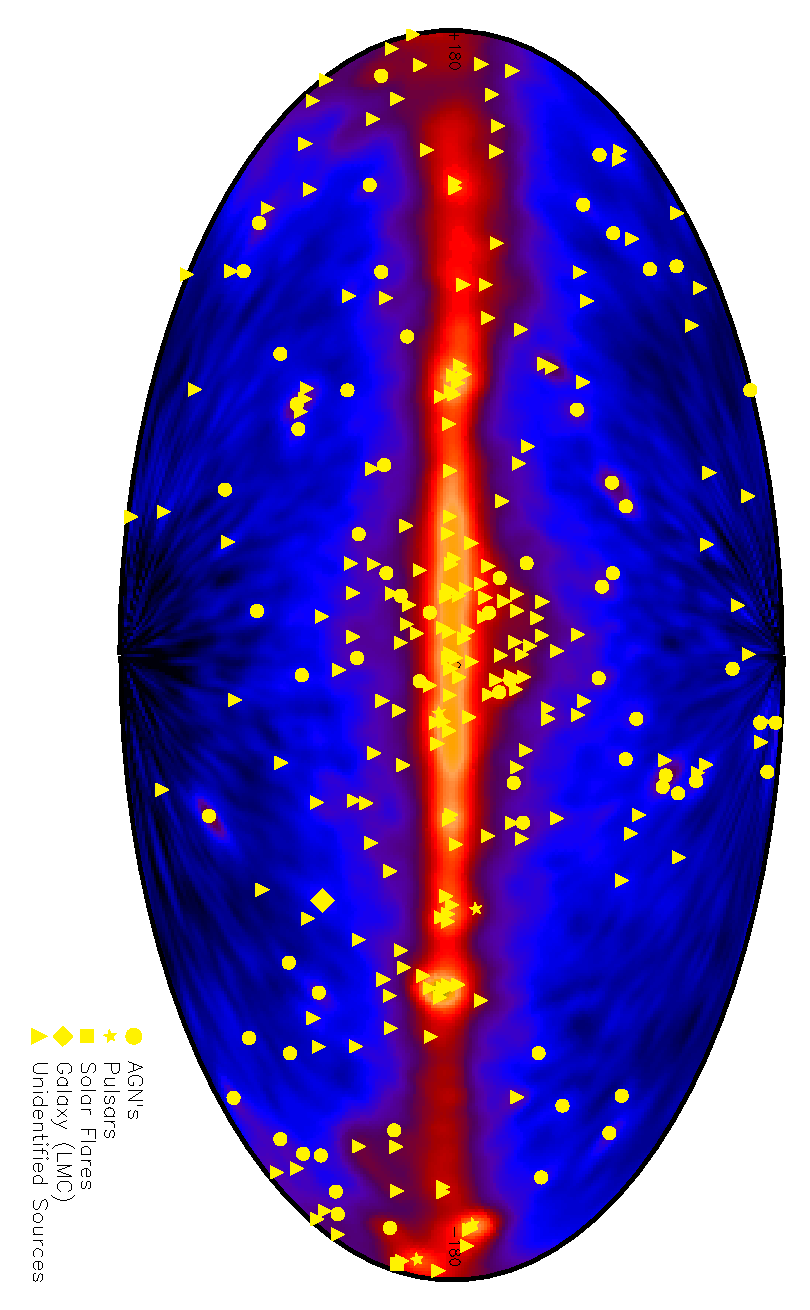
\includegraphics[width=0.8\columnwidth,angle=90]{Figures/3rd_egret_cat.eps} }
	\caption{Third EGRET catalog all-sky map. Unidentified sources represented by triangles. Image courtesy of \url{https://heasarc.gsfc.nasa.gov/docs/cgro/images/epo/gallery/skymaps/}}
	\label{fig:3EGSky} 
\end{figure}

In spite of the difficulties in \egret{} source association, many studies have attempted correlating the unidentified \egret{} sources with various Galactic populations. In particular, several authors found strong evidence for statistical correlation between \glspl{snr} and some of the low-latitude unidentified sources \citep{Sturner95, Esposito96, Romero99}. In a review of the state of potential \snr{} /  \egret{} associations, \cite{Torres03} showed that there were 19 unidentified \egret{} sources that had an \snr~fall within its 95\% error box. Performing Monte Carlo simulations of the population of  \egret~sources, they determined that the chance probability for the 19 sources to be coincident with an \snr~was $1.05 \times 10^{-5}$, implying a probability of 0.99998 that at least one of the associations is real. Despite the statistical correlation of \egret~sources with \glspl{snr}, there were no definitive associations of an \snr~with any \egret~sources.

As the successor to \egret{}, the \lat{} was designed to improve upon its predecessor in a multitude of areas relevant to detecting \snrs{} \citep{atwood09,lat_perf}. The \lat{} has a much improved angular resolution (68\% single-photon containment radius $\sim 0.4^{\circ}$ at 1\gev{} for photons with the best quality direction reconstruction, PSF3 event type, compared to $\sim 1.7^{\circ}$ for \egret{} at the same energy), necessary to resolve \snrs{} as extended objects. The \lat{} also benefits from a superior sensitivity due to a combination of the improved \psf, larger peak effective area ($ {\rm > 9000~cm^2}$ vs. ${\rm \sim 1500~cm^2}$), wider \fov{} (2.4 sr, which is nearly 5 times that of \egret{}), and deeper, more-uniform sky exposure (afforded by the \lat's scanning observations as opposed to \egret's pointing operation). 

This bump in sensitivity results in the \lat{} detecting considerably more sources than \egret. Remarkably, within its first three months of commission, the \lat{} detected 205 sources (above {\rm 10$\sigma$ significance \citep{lat_3m}), and by 11 months, 1451 sources above 4$\sigma$ \citep{1FGL}, compared to  the aforementioned 271 over the entire \egret{} mission. In fact, over its lifetime, \egret{} detected a total of about ${\rm 1.5~x~10^6}$ cosmic photons, while as of March 2016, the \lat{} has detected ${\rm \sim 863~x~10^6}$ source class photons. The \lat's point-source sensitivity peaks between 1 and 10\gev{}, depending on location on the sky. \jamie{plot comparing lat to egret sensitivity?}. With its increased sensitivity and higher energy range (up to $\sim$ 2\tev{} with the recent Pass 8 event reconstruction improvements, which is nearly an order of magnitude higher than \egret{}), the \lat{} is uniquely situated to study the \gam{} morphology and spectra of \snrs{}.

Both energetic lepton interactions (\ie \ic{} radiation of relativistic electrons interacting with ambient photon fields, and nonthermal \brems{}) and hadronic processes ($\pi_0$ decay \gam{}s from \cray{} protons encountering surrounding nuclei) produce spectra observable at \gam{} energies (see Chapter \ref{chap:gamAstr} for details). While the \ic{} generating electron population is also observable through emission of radio \sync{} photons, the proton-proton interaction solely emits \gam{}s. Despite being the prime energy range to observe the effects of cosmic particle acceleration, complexities at the lower \lat{} energy range stymie \snr{} morphology studies.

The \lat{} detects a strong, soft band of diffuse emission in the Galactic plane due to the interactions of  \crs{} with interstellar material. This bright diffuse radiation combined with the multiple potential emission scenarios, broadening \psf{} at decreasing energy, and a high source density in the plane can make it difficult to spatially disentangle sources observed by the \lat{}. To circumvent these 
difficulties, the majority of the analyses undertaken in this thesis are focused on the ${\rm E \geq 1\gev}$ energy range. This energy band is ideal for probing the properties of the accelerated particle populations present in the \snr{} environment. Studies of  \snrs{}  above 1\gev{} benefit from finer \lat{} \psf{}, striking a balance between minimizing the diffuse contribution, maximizing photon sensitivity, and retaining good photon statistics. Furthermore, evolved \snrs{}  exhibit a spectral break between 1-10\gev{}. Explanations for the break range from Alfv\' en wave evanescence generated by collisions of partially ionized material in \mcs{} overtaken by \snr{}  shocks \citep{Malkov11}, reflected shocks in clouds \cite{Inoue10c}, and energy-dependent diffusion from shocks \cite{Ohira11}. Studying \snrs{} in this energy range hones our capability to tackle several goals set out by the \Fermi{} team when the mission was conceived.

Two of the primary science goals of the \lat{}  are to 1. resolve the \gam~sky, uncovering the nature of the unidentified sources detected by \egret{}, and 2. to understand the mechanisms of cosmic particle acceleration \citep{atwood09}. In this chapter, we describe our efforts towards addressing these questions by studying the \gam{} emission coincident with sources comprising the population of known radio emitting \snrs{}.

Prior to this work, several individual studies with the \lat{} had successfully resolved spatially extended emission from \snrs{} \citep[and references therein]{3FGL}, yet no systematic analysis leveraging the \lat{}'s full-sky coverage had yet been performed. We performed a uniform study of the \snrs{} in aggregate to measure the properties common to these objects. An understanding of these common characteristics allows us to assess \snrs{} as a class of \gam{} and \cray{} emitting objects and serves as the impetus for this uniform analysis of the known Galactic \snrs{}. We  report here on the published results from the \snrcat{} \cite{SNRcat}. \jamie{they aren't published yet, but almost maybe that will change by June}
 
 \jamie{2FGL only had 7 ID'd SNR, 4 snr, 58 spp. 3FGL had 12 SNR, 11 snr, 49 spp. I'm not sure what made some snr vs. spp. They must have all been point sources right? No known radio pwn, psr?}

\section{\label{snrCat:ptlk}The \ptlike~  Maximum Likelihood Package}

This section is about the tools (and intricacies there in) developed to study SNRs with Fermi

Describe pointlike and what problems it aims to solve in contrast to gtlike.

pointlike is good at analysis where iteration is key because it takes some shortcuts with some integrals and is faster than gtlike. 

Not sure how much to talk about pointlike here vs. modifiying what's in the next chapter from the snrcat paper. 

The addSrcs framework extends/exploits pointlike 

addSrcs in this section or merged into the next one?

I need to stress that this is not just a tool developed, but there's an art and finesse to it (talk about the problems we overcame), there was much iteration.

tool plus knowledge to get the best result

what are the aspects of addSrcs tht needed knowhow, finagling

\jamie{the following  is from a confluence page motivating and describing  addSrcs}

To attain the best understanding of a source of interest, the best characterization of the corresponding ROI is necessary. This is particularly challenging in dense source and strong diffuse dominated regions (i.e. the Galactic plane). We have developed an automated method for systematically locating and modeling all potential point and/or extended sources in an \roi{} using \ptlike{}. This work started as a parallel and complementary analysis to the SNR cat pipeline, intended to minimize possible bias introduced by the initial model for an ROI (e.g 2FGL) It is  used to derive the input sources model for the SNR catalog. The goal of this work is to use this "add sources" method to aid in characterization of GeV emission near SNRs and nearby molecular clouds.

what are some motivations for various addSrcs decisions 

How to distinguish addSrcs from how addSrcs was applied to the SNR cat. For the SNRcat, it was addSrcs in PS mode with specifics relevant to the SNR cat needs (like what?)


Describe how we put together/designed this analysis what questions were we trying to answer?


tested pipeline with 6 sources (I have the tests somewhere, see old Fermi symp poster, Gal Evo too)
\section{Input Source Model Construction}\label{snrCat:AddSrcs}

\jamie{add some more bkg on the SNR cat here and add more of the snrCat intro}


To characterize each candidate SNR we constructed a %n optimal 
model of \g-ray emission in the RoI which includes all significant sources of emission as well as the residual background from CRs misclassified as \g-rays. We implemented an analysis method to create and optimize the \jamie{fill this in }~models for each of the 279 RoIs. For each RoI, we started with all sources listed in 
%We started with a list of cataloged sources within our RoI from 
the \twofgl \citep{2FGL}, based on $2$\,years of Source class data, within the RoI. To this we add pulsars from \twopc \citep{2PC}, based on $3$\,years of source class data, with 2PC taking precedence for sources that exist in both. 
For the diffuse emission we combined the standard IEM corresponding to our P7 data set, gal\_2yearp7v6\_v0.fits, with the standard %. To this we added a 
model for isotropic emission, which accounts for extragalactic diffuse \g-ray emission and residual charged particles misclassified as \g-rays. 
%We used the standard IEM corresponding to our P7 data set, gal\_2yearp7v6\_v0.fits, and the 
Both the corresponding isotropic model, iso\_p7v6source.txt, and the IEM are the same as used for the 2FGL catalog analysis\footnote{Further details on the diffuse emission models are available at \url{http://fermi.gsfc.nasa.gov/ssc/data/access/lat/BackgroundModels.html}}.
% Files used are equivalent to FSSC models: ring_2year_P76_v0.fits, isotrop_2year_P76_source_v0.txt

%To better optimize our model, 
Compared to 2FGL, we used an additional year of data and limited the energy range to $1-100$\,GeV. This can result in different detection significances and localizations than previously reported in 2FGL. To account for these effects, we recreated the RoIs' inner $3$\degr{}\,radius regions, which encompass the radio extents of all known SNRs, observed to be $\leq 2.6$\degr{} and allows a margin for the LAT PSF. 
The weighted average $68\%$~containment radius of the LAT PSF for %front and back converting 
events at $1$\,GeV is $\sim0.7$\degr{} \citep{lat_cm}. 
We note that this implicitly assumes that an SNR's GeV extent should not be more than about an order of magnitude larger than its radio extension and also note that the selection biases stated in Green's catalog limit the range of known SNRs' radio extensions. 

To build the inner $3$\degr{}\,radius model of each RoI, we first removed all sources except identified Active Galactic Nuclei (AGN) and pulsars, whose positions on the sky are independently confirmed by precise timing measurements \citep{2PC}. Retained AGN were assigned their 2FGL positions and spectral model forms. Pulsars' positions and spectral forms were taken from 2PC. 2FGL sources identified or associated with SNRs are removed when they lie within the inner $3$\degr{}. %The removal included SNRs included in 2FGL. 

We generated a map of source test statistic (TS) defined in \citet{Mattox96} via \ptlike{} on a square grid with $0.1$\degr{}\,$\times$\,$0.1$\degr{} spacing that covers the entire RoI. \ptlike{} employs a binned maximum likelihood method. The source TS is defined as twice the logarithm of the ratio between the likelihood~$\mathcal{L}_1$, here obtained by fitting the model to the data including a test source, and the likelihood~$\mathcal{L}_0$, obtained here by fitting without the source, i.e., $\textrm{TS = 2 log}(\mathcal{L}_1/\mathcal{L}_0$). At the position of the maximum TS value, we added a new point source with a Power Law (PL) spectral model:
%\terri{\g{} is implicitly negative here but is used as positive everywhere in the pipeline and following plots. Verify that setting to explicitly positive here works for sections between here and pipeline results.} \jack{done.}
\begin{equation}
	\label{eqn:PL}
	\frac{dN}{dE} = N\frac{(-\Gamma+1)E^{-\Gamma}} {E_{\rm max}^{-\Gamma+1} - E_{\rm min}^{-\Gamma+1}}
\end{equation}
where $N$ is the integrated photon flux, $\Gamma$ is the photon index, and $E_{\rm min}$ and $E_{\rm max}$ are the lower and upper limit of the energy range in the fit, set to $1$\,GeV and $100$\,GeV, respectively.
We then performed a maximum likelihood fit of the RoI to determine $N$ and $\Gamma$ and localized the newly added source. 
The significance of a point source with a PL spectral model is determined by the $\chi^2_n$ distribution for $n$ additional degrees of freedom for the additional point source, which is typically slightly less than~$\sqrt{\textrm{TS}}$\footnote{See \url{http://fermi.gsfc.nasa.gov/ssc/data/analysis/documentation/Cicerone/Cicerone_Likelihood/TS_Maps.html} for further details.}.

To promote consistent convergence of the likelihood fit, we limited the number of free parameters in the model. For sources remaining after the removal step, described above, we freed the normalization parameters for the sources within $5$\degr{} of the RoI center, including identified AGN and pulsars. For 2FGL sources between $5$\degr{} and $10$\degr{}, we fixed all parameters. The spectrum of the IEM was scaled with a PL whose normalization and index were free, as done in 2FGL.
%\terri{why is this reference here?} \jack{same as done in 2FGL}. 
For the isotropic emission model, we left the normalization fixed to the global fit value since the RoIs are too small to allow fitting %separately fit 
the isotropic and Galactic IEM components independently. The isotropic component's contribution to the total flux is small compared to the IEM's at low Galactic latitudes.

After localizing them, the new sources were tested for spectral curvature. In each of the $4$~energy bands per decade we calculated the TS value for a PL with spectral index fixed to $2$ and then summed the TS values. 
%We summed TS values for fits in individual energy bands, each calculated in an energy band for a PL model of fixed spectral index~$2$, with $4$~energy bands per decade. 
We refer to this as $\mathrm{TS_{band fits}}$. A value for $\mathrm{TS_{band fits}}$ much greater than the TS calculated with a PL ($\mathrm{TS_{PL}}$) suggests with a more rapid calculation that the PL model may not accurately describe the source. %, where $\mathrm{TS_{PL}}$ is the TS with a PL fit. 
Analogously to 2FGL \citep{2FGL}, we allow for deviations of source spectra from a PL form by modeling sources with a log-normal model known colloquially as LogParabola or logP:
\begin{equation}
	\newcommand{\pfrac}[2]{\left(\frac{#1}{#2}\right)} \frac{dN}{dE} = N_0\pfrac{E}{E_b}^{-(\alpha + \beta\log(E/E_b))}
	\label{eqn:logP}
\end{equation}
where $N_0$ is the normalization in units of photons/MeV, $\alpha$ and $\beta$ define the curved spectrum, and $E_b$ is fixed to $2$\,GeV. If $\mathrm{TS_{band fits} - TS_{PL}} \geq 25$, we replaced the PL spectral model with a logP model and refit the RoI, including a new localization step for the source. We retained the logP model for the source if the global \logL{} across the full band improved sufficiently: 
$\mathrm{TS_{curve}} \equiv 2 ($\logL{}$_{\mathrm{logP}}-$\logL{}$_{\mathrm{PL}}) \geq 16$. 
Otherwise we returned the source to the PL model which provided the better global \logL. Across all RoIs, less than $2\%$ of the newly added sources retained the logP model. 

We continued iteratively generating TS maps and adding sources within the entire RoI until additional new sources did not significantly change the global likelihood of the fit. The threshold criterion was defined as obtaining $\mathrm{TS < 16}$ for three consecutively added new sources, denoted as $\mathrm{N_{TS < 16} = 3}$. Despite iteratively adding a source at the location of the peak position in the TS map, the TS values of new sources may not decrease monotonically with iteration for several reasons. First, source positions were localized after fitting the RoI and generating the TS map. Second, some added sources were fit with a more complex spectral model than a simple PL. Finally, when creating the TS map, we fixed the source's spectral index to $2$, whereas when adding the actual source to the model, we allowed its index to vary. 

The specific value of $\mathrm{N_{TS < 16} = 3}$ was chosen to avoid missing sources with $\mathrm{TS \geq 25}$, the threshold commonly used for source detection in LAT data, and to optimize computation time. We tested the threshold by selecting eight representative SNRs from both complex and relatively simple regions of the sky, with both hard and soft spectral indices. We applied the above procedure to the test RoIs using a criterion of $\mathrm{N_{TS < 16} = 6}$ and counted how many $\mathrm{TS \geq 25}$ sources would be excluded if a smaller $\mathrm{N_{TS < 16}}$ criterion was used. Reducing the threshold to $\mathrm{N_{TS < 16} = 3}$ cut only one significant source in any of the regions. Since the maximum number of sources added in any test RoI was $38$, the minimum $14$, and the total number of sources added across all test regions was $221$, we chose to use $\mathrm{N_{TS < 16} = 3}$ for the full sample. To allow for proper convergence of the likelihood fit, we reduced the number of free parameters prior to each new source addition. If the previously added source was between $3$\degr{} and $5$\degr{} of the center of the RoI, just its normalization was freed, and if greater than $5$\degr{} all its source parameters were fixed.

To avoid having newly added sources overlap with pulsars, we deleted new sources from the RoI if they were within~$0.2$\degr{} of a \g-ray pulsar and refit the pulsar in the $1-100$\,GeV range following the 2PC conventions. 
2PC modeled pulsar spectra as PL with an exponential cutoff (PLEC),
\begin{equation}
	\newcommand{\pfrac}[2]{\left(\frac{#1}{#2}\right)} \frac{dN}{dE} = N_0 \pfrac{E}{E_0}^{-\Gamma} \exp\left(-\frac{E}{E_c}\right)^{b},
	\label{eqn:PLEC}
\end{equation}
where \textit{$N_0$} is the normalization factor, \textit{$\Gamma$} is the photon spectral index, \textit{$E_c$} the cutoff energy, and $b$ determines to the sharpness of the cutoff. 2PC assessed the validity of fixing $b$ to $1$ in Equation~\ref{eqn:PLEC} (PLEC1) 
%Fixing $b$ in Equation \ref{eqn:PLEC} to $1$ (PLEC1),  the PLEC1 model, 
by repeating the analysis using a PL model, as well as the more general exponentially cut off PL form, allowing the parameter $b$ in Equation~\ref{eqn:PLEC} to vary. For the pulsar spectra in this analysis, we compared the maximum likelihood values for spectral models with and without a cutoff and with and without the value of $b$ being free, via %model's likelihoods as: 
$\mathrm{TS_{cut}} \equiv 2 ($\logL{}$_{\mathrm{PLEC1}}-$\logL{}$_{\mathrm{PL}})$ and $\mathrm{TS}_{b} \equiv 2 ($\logL{}$_{\mathrm{PLEC}}-$\logL{}$_{\mathrm{PLEC1}})$ to determine which to use. If $\mathrm{TS_{cut}} < 9$ is reported for the pulsar in 2PC then a PL model is used. If TS$_{\mathrm cut} \geq 9$, we then check to see if the cutoff energy fit in 2PC lies within the restricted energy range of $1-100$\,GeV used in this work. For pulsars with cutoffs $\geq 1$\,GeV, we then use the PLEC model if TS$_{\mathrm b} \geq 9$, and the PLEC model with cutoff freed otherwise. %\terri{This says you use the free b PLEC regardless of $\mathrm{TS}_{b}$'s value, which can't be right.} 
For those pulsars with cutoffs less than 1 GeV the spectral parameters are fixed to the 2PC values.

%\[ \begin{dcases*}
%        \mathrm{PLEC} & if TS$_{\mathrm b} \geq 9$ \\
%        \mathrm{PLEC1} & if TS$_{\mathrm b} < 9$ and TS$_\mathrm{cut} \geq 9$ \\
%        \mathrm{PL} & if TS$_\mathrm{cut} < 9$
%        \end{dcases*}
%\]
%\terri{Jamie (Jack?), please verify this. NB: I derived this from the text (now in comments) and there are cases oddly covered here, e.g. of TS$_{\mathrm b} \geq 9$ \&\& TS$_\mathrm{cut} < 9$ is nominally doubly specified as both PLEC and PL, while TS$_{\mathrm b} < 9$ \&\& TS$_\mathrm{cut}  < 9$ seems to be both a PLEC1 and a PL).}
%\jack{This is what was done in addSrcs, but not what was done in the pipeline, where I had to explicitly add in the 2PC pulsar results as the first step in the model. Text has been re-written to reflect how pulsars are handled in the pipeline using 2PC.}

% a PLEC model for a pulsar if $\mathrm{TS_{b}} \equiv 2 ($\logL{}$_{\mathrm{PLEC}}-$\logL{}$_{\mathrm{PLEC1}}) \geq 9$,
%%%$\mathrm{TS_{b} \equiv 2\Delta log( likelihood) \geq  9}$between PLEC1 and PLEC,
%PLEC1 if $TS_{b} < 9$ 
%\[  
% \mathrm{TS_{cut}} \equiv 2(\log \mathcal{L}_{\mathrm{PLEC1}}-\log \mathcal{L}_{\mathrm{PL}}) \begin{dcases*}
%        \mathrm{PLEC1} & if TS$_{cut} \geq 9$ \\
%         \mathrm{PL} & if TS$_{cut} < 9$
%        \end{dcases*}
%\]
%and $\mathrm{TS_{cut}} \equiv 2 ($\logL{}$_{\mathrm{PLEC1}}-$\logL{}$_{\mathrm{PL}}) \geq 9$
%%$\mathrm{TS_{cut} = \Delta log(likelihood) \geq 9}$ between PLEC1 and PL,
%, and finally, if $\mathrm{TS_{cut} < 9}$ we used a PL spectral model. 

To complete the construction of our point source RoI model, we took the output of the previous steps and removed all sources with TS~$< 16$. This final model was then used as the starting model for analyzing candidate SNR emission. We conservatively allow sources with TS down to $16$ $(\sim4\,\sigma)$ in order to account for the effects of at least the brightest sub-threshold sources on the parameter fits for the other sources in the model. Furthermore, while the SNR analysis method described in the next subsection (\ref{Sec:DetectMethod}) is allowed to remove sources, it cannot add them. Thus we start from a set of sources designed to allow the final model to capture all significant emission within the central region. To corroborate our method of systematically adding sources to a region, we compare our RoI source models with those found by the 2FGL approach in Appendix~\ref{appen:addSrcs2FGL}. 


\section{Comparison of Source Models with 2FGL}
\label{snrcat:addSrcs2FGL}

This SNR catalog was constructed using $3$~years of P7 Source class data in the energy range $1-100$\,GeV, whereas 2FGL used $2$\,years of data over the larger energy range $0.1-100$\,GeV. The differences in observing time and energy range resulted in residual, unmodeled emission in some RoIs as well as changes to some 2FGL sources' spectral model, position localization, and detection significance. Here we compare the input source models constructed for this catalog, described in Section~\ref{Sec:AddSrcs}, with 2FGL to better understand the method's ability to describe the regions studied. Since we rederive the input source model only within a $3\degr$\,radius of the center of each RoI, 
%removed from our source model all 2FGL sources within a $3\degr$\,radius of the center of each RoI except those identified as AGN and pulsars, 
we consider sources only inside that radius.

Given the data set differences, in each RoI we expect similar but not identical numbers of sources relative to those in 2FGL.
Figures~\ref{fig:2FGLvAddSrcs} and \ref{fig:2FGLvAddSrcsAssoc} show the numbers of significant (TS\,$\geq 25$) 2FGL sources and derived input model sources (excluding 2FGL identified AGN and pulsars kept in the input model) in individual RoIs as 2D histograms. In Figure~\ref{fig:2FGLvAddSrcs}, 
the number of sources in the derived input model is typically greater than the number of 2FGL sources that are significant at $1-100$\,GeV. 73 of the 279 RoIs studied contain at least one of the the 12 extended 2FGL sources. Since 2FGL extended sources were removed from the inner $3\degr$ of each RoI, and this region was repopulated with point sources, we can detect multiple point sources inside the extent of any removed extended 2FGL sources. This decomposition of extended sources, combined with the longer data set and different energy range compared to 2FGL, contribute to the high ratio of input model to 2FGL sources in some RoI, which demonstrates the need to rederive the source model. %Included among these newly added sources are sources that may not be coincident with a 2FGL source. 

\begin{figure}[h!]
	\centering
	\makebox[\linewidth]{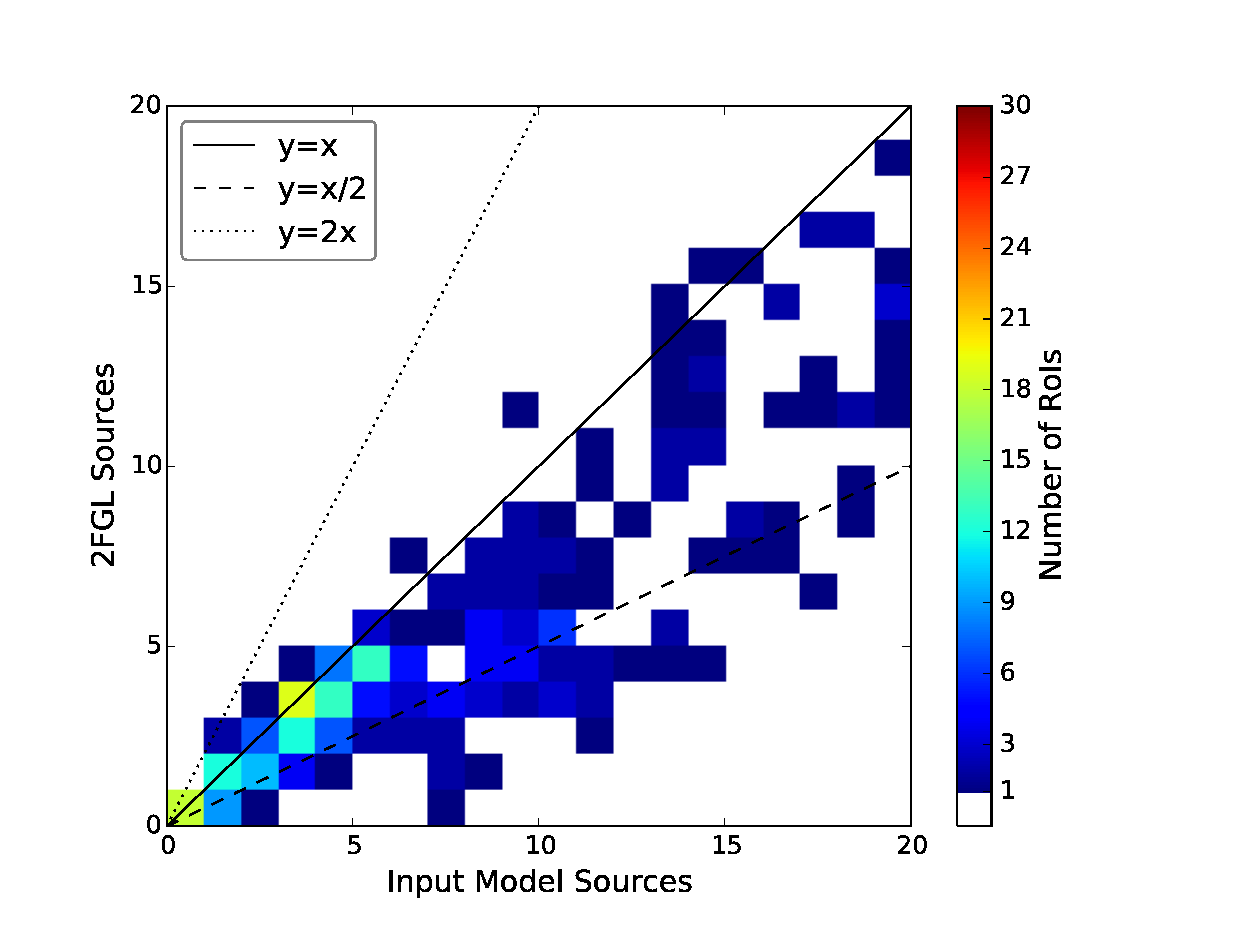
\includegraphics[width=0.8\columnwidth]{figures/addSrcs_2FGLnoAGNPSR_TSgt25_in3deg_2dhist_maj.eps} } 
	\caption{Comparison of the number of 2FGL sources with TS$_{1-100\,\mathrm{GeV}} \geq 25$ (excluding AGN and pulsars) with the number of newly added input model sources in the present analysis, for sources within $3$\degr{} of the center of each RoI. The color scale shows the number of RoIs with a particular combination of numbers of 2FGL sources and new sources.
		%The color scale shows the number of RoIs with a particular ratio of 2FGL to new sources. 
		White corresponds to no RoI with that combination of source counts.}
	%\terri{We are exploring the reasons why there could be more or fewer sources of a given type in an RoI. For instance, multiple addSrcs sources could be associating to the same 2FGL source. There are also cases where the added source is close by not quite within  $0.2$\,\degr{} of the 2FGL source.}
	\label{fig:2FGLvAddSrcs} 
\end{figure}

To more accurately represent the 2FGL sources being reproduced in the central $3\degr$, in Figure~\ref{fig:2FGLvAddSrcsAssoc} we limited the input model sources to those within $0.2\degr$ (approximately the width of the core of the $10$\,GeV PSF) of a 2FGL source, effectively excluding input sources that are not co-spatial with a 2FGL source. Here we see that the majority of 2FGL sources have counterparts in the rederived set. 
As a region's complexity increases, seen as an increase in numbers of 2FGL sources, up to about half of the 2FGL sources may not have counterparts within $0.2$\degr. Given that in these same regions we have more new sources than 2FGL sources, as seen in Figure~\ref{fig:2FGLvAddSrcs}, we find as expected that the longer data set with improved statistics at higher energies, where the angular resolution of the LAT is the best, allows us to add new sources to account for newly significant excesses in these complex regions. 
%As mentioned above, we do not expect to precisely reproduce the results of 2FGL. 
Additionally, sources with low TS in 2FGL are particularly susceptible to having a newly added source which may start at a similar position but then localize further than $0.2\degr$ from the 2FGL source. 

Thus, we find that the method developed and used here produces a model which reproduces the 2FGL sources as expected, including differences that trend as anticipated given the longer data set and modified energy range, yielding better spatial resolution. The new method thus provides reasonable representations of the regions being modeled as input for the final analysis.

%\terri{Suggest removing (the remainder of) this paragraph.} 
%Additional discrepancies between our source model and 2FGL can arise from shifting of source position of low TS 2FGL sources \terri{2FGL sources can't shift positions...} (i.e. newly added sources separated from a 2FGL source by more than $0.2\degr$, particularly sources with high flux neighbors), and association of 2FGL sources with newly added sources outside $3\degr$ (and vice versa) \terri{Per Section~\ref{Sec:AddSrcs}, we're not removing or adding sources outside $3\degr$, so why is this the case?}. Despite this, Figure \ref{fig:2FGLvAddSrcsAssoc} shows that in many RoI, our source model recovered most of the 2FGL sources.


% % %
\begin{figure}[h!]%[t] 
	\centering
	\makebox[\linewidth]{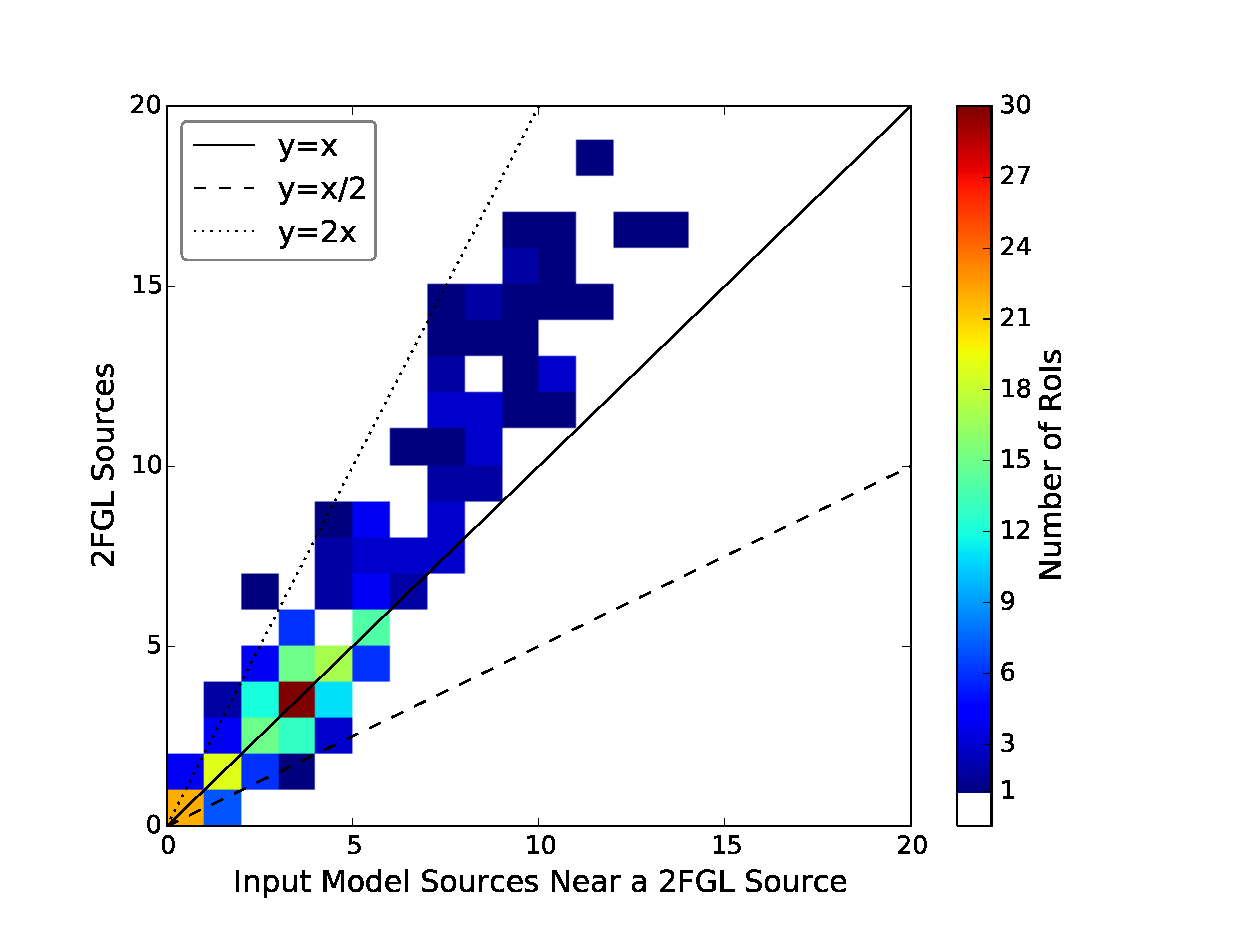
\includegraphics[width=0.8\columnwidth]{figures/addSrcsWassoc_2FGLnoAGNPSR_TSgt25_in3deg_2dhist_maj.eps} }
	\caption{Same as Figure~\ref{fig:2FGLvAddSrcs}, including only input model sources lying within $0.2$\degr{} of a 2FGL source.}% within $3$\degr{} of the center of an RoI and with TS$_{1-100\,\mathrm{GeV}} \geq 16$, .}
	\label{fig:2FGLvAddSrcsAssoc} 
\end{figure}
% % %

\section{SNR Catalog Results}
\label{snrCat:results}
What to include from SNR cat

Pull parts of the intro/abstract as needed.

sections: 2, 2.1, 2.2, 2.3 (do I need 2.3.1, 2.3.2)

 First par of 3.1 about how we classify. Summarize some of the relevant catalog results of section 3.2. There's no real reason to include the catalog tables I think. Parts of 3.2.1 3.2.2, 3.2.3 just to highlight which sources were newly detected. 
 
 What to include from section 4? I didn't make these plots, but I contributed to the pipeline script and gave advice on things. 
 
 For the mock snrCatalog, I didn't do the analysis, but I ran addSrcs on the mock sources. maybe there's not much to say about this though.

Section 5? It's not my work, but I participated in discussions, edited text in the section a little bit. I think something needs to be included from this because one of the points of the paper was to see what we could say about the total energy in CR in the Galaxy

Parts of conclusion

Which figure to include from snr cat results?


\section{Summary}\label{snrCat:summ}
In this chapter, we have presented results from the publication of the \snrcat. Application of addSrcs adding point sources to characterize emission in an\roi. Give more details on validation and testing than was given in the paper, as well as details on the code. Work on fitting single extended source, present some work on detected SNRs and population properties, implications for total power in cosmic rays (don't focus on this because it wasn't where I contribute the most). Mock catalog contributions. Testing with extended sources or don't mention too much because we decide not to apply it here?

With its unprecedented sensitivity and angular resolution above 1\gev, the \lat~provides for the first time the opportunity to distinguish SNR-emitted photons from their backgrounds, and  to unambiguously detect and identify dozens of \glspl{snr}. \jamie{maybe this is for the intro/abstract because it's a little vague}

The \lat{} is uniquely situated to address these goals and definitively detect and identify dozens \snrs

Focus our efforts on
\section{Scratch}
has the spatial and spectral sensitivity to resolve

good spatial and spectral 


talk about how much "power" comes from the higher energy  range,

EGRET point source sensitivity is ${\rm \sim1x10^{-7}}\flux{}$
 \url{http://fermi.gsfc.nasa.gov/science/instruments/table1-1.html} get this number from somewhere else


\jamie{somewhere I should also say that identifying an extended source as such gives better spectra, see 2FHL}

\cite{Thomson93}, egret observed a total of 1.5 million celestial \gam{}

\jamie{ Fermi goals: 1. Resolve the \gam~sky: the origins of diffuse emission and the nature of unidentified sources: Source identification through good source localization, measurement of spectra across broad energy range, nearly continuous monitoring of the sky for temporal variability
	2. Understand the mechanisms of particle acceleration in celestial sources:}

\jamie{understanding accel plus identification of the potential SNRs motivates the SNR cat }

\jamie{snrs as source of Galactic cosmic rays, and thus as drivers of Galactic evolution}

-what's to gain from studyng the population vs individual?

-constraint on CR energy density in the Galaxy

-do the observed g-ray properties match those
of models?

-like index etc?
\chapter{Extended Source Detection above 50 GeV: The 2FHL Catalog}
\label{chap:2FHL}

\section{Introduction}\label{2FHL:intro}
\jamie{give this a different title
    }
The \lat{} \citep{atwood09} on board the \Fermi{}
\gam{} space telescope has been surveying the whole sky since August 2008.
Its unprecedented sensitivity and localization accuracy allowed the detection
of over 3,000 point-like sources in  4\,years of data \citep[see the
third catalog of {\it Fermi}-LAT sources, 3FGL, ][]{3FGL}.
Typically, {\it Fermi}-LAT catalog studies are based on  source detection
and characterization in the whole 0.1\,GeV--100\,GeV energy band.
The larger photon statistics present at low energy, counterbalanced by
the LAT point-spread function (PSF) whose size decreases with energy,
yields an optimum sensitivity at a energies of a few GeV.
The {\it Fermi}-LAT catalogs are thus representative of the GeV sky
more than they are of the MeV or the sub-TeV sky.


The first {\it Fermi}-LAT catalog of hard sources, named 1FHL \citep{1FHL}, provided an unbiased census of the sky at energies from 10~GeV up to 500~GeV. %The comparison of 1FHL and 0.1--100\,GeV observations \citep[as provided in][]{2FGL} allowed us to uncover the presence of spectral breaks and to determine that  blazars of the BL Lacertae (BL Lac) type represented about 50\,\%of the entire source population { detected in that band}.
{ All-sky surveys at $\gamma$-ray energies} are instrumental for ground-based imaging atmospheric Cherenkov telescopes (IACTs) such as H.E.S.S., MAGIC, and VERITAS \citep[][respectively]{holder08,lorenz04,hinton04}
in order to find new sources because of their limited fields of view (FoV).


Recently, a new event-level  analysis (known as Pass 8) has been developed by the \emph{Fermi}-LAT collaboration \citep{atwood13b,atwood13}. Pass~8 significantly improves the LAT's background rejection, PSF, and effective area. All these  enhancements lead to a significant increase of the LAT sensitivity and its effective energy range, from below 100~MeV to beyond a few hundred GeV  \citep{atwood13b,atwood13}. These improvements are particularly significant above 50\,GeV, yielding an enhancement in the acceptance and PSF by a factor  between 1.2 and 2. 
It is interesting to note that, above 50\,GeV, both the PSF (governed mostly by the pitch of the tracker silicon strips and the spacing of the tracker planes, see Chapter \ref{FGST:LAT}) and the effective area of the LAT are only weakly dependent on energy and that the LAT 
operates, due to the (almost complete) absence of background, in the photon-limited regime.

We use 80\,months of Pass~8 data to produce a catalog of sources detected by the LAT at energies\footnote{Note the different energy range with respect to the 1FHL.} between 50\,GeV and 2\,TeV. This constitutes the second catalog of hard \lat{} sources, named \twofhl{}\jamie{add the if I haven't wrote 2fhl somewhere else yet}, which allows a thorough study of the properties of the whole sky in the sub-TeV domain. In this thesis, we present results published in \cite{2FHL}, exclusively focusing on the Galactic science analysis and results and eschew the extragalactic results to the published \twofhl{} paper \jamie{move this last sentence to the beginning and italicize?}.


%%%%%%%%%%%%%%%%%%%%%%%%%%%%%%%%%%%%%%%%%%%%%%%%%%%%%%%%%%%%%%%%
%
%         Analysis 
%
%%%%%%%%%%%%%%%%%%%%%%%%%%%%%%%%%%%%%%%%%%%%%%%%%%%%%%%%%%%%%%%%
\section{Analysis}
\label{sec:analysis}


%%%%%%%%%%%%%%%%%%%%%%%%%%%%%%%%%%%%%%%%%%%%%%%%%%%%%%%%%%%%%%%%
%
%         Detection
%
%%%%%%%%%%%%%%%%%%%%%%%%%%%%%%%%%%%%%%%%%%%%%%%%%%%%%%%%%%%%%%%%
% \subsection{\label{sec:sourceDetect}Data Selection and Source Detection}

\subsection{\label{sec:data_sel}Data Selection}


We use 80 months (from August 2008 to April 2015) of P8\_SOURCE 
photons with reconstructed energy in the 50\,GeV--2\,TeV range.
At these energies the LAT has an energy resolution of around 10--15\,\% (1\,$\sigma$).
Photons detected at zenith angles larger than 105$^{\circ}$ were excised
to limit the contamination from $\gamma$-rays generated by cosmic-ray
interactions in the upper layers of the atmosphere. Moreover, data were filtered
removing time periods when the instrument was not in sky-survey mode\footnote{This
    was achieved using the expression `(DATA\_QUAL$>$0)\&\&(LAT\_CONFIG==1)' in {\tt gtmktime}.}.
This leaves
approximately 61,000 photons detected across the entire  the sky. The count map
reported in Figure~\ref{fig:skymap} shows that the \lat{} observes
many point-like sources and
large scale diffuse emission in the direction of our Galaxy, some of which appears
coincident  with the so-called {\it Fermi} bubbles \citep{su10,lat_bubbles}.



\begin{figure*}[!ht]
    \begin{centering} 
        \includegraphics[width =\textwidth]{Figures/all-sky_countmap-Marco.eps}
        \caption{Adaptively smoothed count map in the 50\,GeV--2\,TeV band represented in Galactic coordinates and Hammer-Aitoff projection. The image has been smoothed with a Gaussian kernel whose size was varied to achieve a minimum signal-to-noise ratio under the kernel of 2. The color scale is logarithmic and the units are counts per (0.1\,deg)$^2$.
            \label{fig:skymap}}
    \end{centering}
\end{figure*}


\subsection{\label{2fhl:sourceDetect}Source Detection}


The first step of the source detection stage comprises the identification of source seeds, which are locations of potential sources whose significance is later tested through a maximum likelihood (ML) analysis. The seed detection method, described further in \cite{2FHL}, includes all the point sources detected in the 1FHL catalog. We note that  this seed list may include statistical fluctuations as well as real sources with a non-optimal position.

A full ML analysis is then performed in order to verify which,
among the seeds, are the reliable sources. 
The analysis is performed in 154 \rois{}, varying between 10$^{\circ}$ and 20$^{\circ}$ in radius, whose sizes and positions in the sky are optimized to cover all the seeds, ensuring that no more than 45 seeds are contained in a single \roi{}.
For each \roi{}, we build
a sky model that includes all the potential sources in the region
as well as the  Galactic and isotropic diffuse emissions\footnote{We~used~the~{\tt gll\_iem\_v06.fits}~and~{\tt iso\_P8R2\_SOURCE\_V6\_v06.txt}
    templates available at \\
    http://fermi.gsfc.nasa.gov/ssc/data/access/lat/BackgroundModels.html.}.
These models, which are defined only up to $\sim$600\,GeV and  $\sim$900\,GeV respectively, where extrapolated up to 2\,TeV.
The \roi{} models include also the extended sources present in the region (see Chapter \ref{2fhl:extended}).
The model is fit to the data via the unbinned ML algorithm provided
within the {\it Fermi} Science Tools\footnote{Available at 
    http://fermi.gsfc.nasa.gov/ssc/data/analysis/software/.} (version v9r34p3).

The spectrum of each source is modeled with a power law because
none of the sources is expected to show statistically
significant spectral
curvature detectable by the LAT in this energy band. 
Indeed, this was the case for the sources in the 1FHL catalog \citep{1FHL}.

The fit is performed iteratively in order to ensure convergence and 
to produce an optimal solution. It proceeds as follows:

\begin{enumerate}
    \item Complex ML fits require approximate knowledge of the 
    starting values of the parameters. For this reason the first
    step  aims to find those values  by fitting each single source separately 
    to determine approximate spectral parameters.
    Throughout the entire process, the parameters of the diffuse emission
    models are left free to vary.
    The significance of each source is evaluated using the test statistic  
    ${\rm TS}=2(\ln \mathcal{L}_1 - \ln \mathcal{L}_0)$, where $\mathcal{L}_0$ and $\mathcal{L}_1$
    are the likelihoods of the background (null hypothesis) and 
    the hypothesis being tested (\eg{} source plus background). 
    At each step in the procedure, marginal sources, those with TS $<$ 10, are removed from the model.
    Once the spectral parameters and significance of each source have
    been evaluated, a global fit for which all the parameters of the sources
    with a ${\rm TS}\geq 10$ are allowed to  vary is performed. 
    Then one more global fit is performed after removing all the sources that had ${\rm TS}< 10$ at the previous global fit.
    This step,
    as well as all the others, includes sources that
    are spatially extended (see Chapter \ref{2fhl:extended});
    
    \item In this second step, the positions of point-like sources, using the best-fit sky model
    derived at step 1, are optimized using the {\tt gtfindsrc} tool. This step
    is done iteratively as well by optimizing first the positions of the
    most significant sources found at step 1 and later  those of the fainter
    ones;
    
    \item The parameters and significances of sources are estimated again (as in step 1) using the best-fit source positions. This step produces the best-fit sky 
    model for any given \roi{}. 
    Seeds with $10\leq {\rm TS}<25$ are included in the model, but not reported in the final catalog;
    
    \item For each source we estimate the energy of the \hep{}
    that the fit attributes robustly  to the source model. This is done using the tool {\tt gtsrcprob} and selecting the HEP that has a probability $>85$\,\% to belong to the source;
    
    \item A  spectrum with three logarithmically spaced bins (boundaries of 50\,GeV, 171\,GeV, 585\,GeV, 2\,TeV) is generated for each source in the \roi{} that is detected with ${\rm TS}\geq 25$ and with the number of detected $\gamma$ rays (estimated by the likelihood, N$_{\rm pred}$) to be $\geq$3.
    
    
\end{enumerate}

The procedure described above achieves the detection of 360 sources (including
the extended sources discussed next in Chapter \ref{2fhl:extended}) 
with TS $\geq$ 25 and N$_{\rm pred}\geq3$ across the entire sky.
The number of seeds kept in the \roi{} models
with $10\leq{\rm TS}<25$ is 453, while 7 are seeds with ${\rm TS\geq}25$, but N$_{\rm pred}<3$.
\jamie{took out the monte carlo sims reasoning for Npred}
%We have performed seven Monte Carlo simulations of the $>$50\,GeV sky whose data have been analyzed like the real data (as detailed above). The  N$_{\rm pred}$ cut was introducedon the basis of these simulations to limit to $\lesssim$1\,\% the number of false positives in the final catalog. These simulations will be discussed in a forthcoming publication.

%%%%%%%%%%%%%%%%%%%%%%%%%%%%%%%%%%%%%%%%%%%%%%%%%%%%%%%%%%%%%%%%
%
%         Extended Sources
%
%%%%%%%%%%%%%%%%%%%%%%%%%%%%%%%%%%%%%%%%%%%%%%%%%%%%%%%%%%%%%%%%
\section{Search for Spatially-Extended Sources}
\label{2fhl:extended}


Preliminary runs of the source detection method described in Chapter \ref{2fhl:sourceDetect} detected clusters of point sources in the Galactic plane, which were suggestive of spatially extended sources. It is also possible that clusters of seed sources, each with sub-detection-threshold significance, could be detected as a significant extended source. 
Not modeling extended $\gamma$-ray emission as such can lead to inaccurate measurements of spectral and spatial properties of both the extended source and neighboring point sources, particularly in the Galactic plane \citep{Lande12}. Most of the TeV sources in the Galactic plane are spatially
extended  \citep{carrigan2013, ong2013}, 
so to clearly connect LAT detections spectrally to these sources, extension detection and characterization is important.
In the following, we distinguish between sources whose extension
have been previously determined with {\it Fermi}-LAT and
new extended sources that are reported for the first time
in a \lat{} catalog. The details of all significantly
detected extended sources are reported  in Chapter \ref{2fhl:ESresults}. 

%%%%%%%%%%%%%%%%%%%%%%%%%%%%%%%%%%%%%%%%%%%%%%%%%%%%%%%%%%%%%%%%
%
%         Extended Sources in 3FGL
%
%%%%%%%%%%%%%%%%%%%%%%%%%%%%%%%%%%%%%%%%%%%%%%%%%%%%%%%%%%%%%%%%

\subsection{\label{2fhl:3FGL_ES}Extended Sources Previously Detected by the LAT}
We explicitly modeled sources as spatially extended when a previous, dedicated, analysis found the source to be resolved by the LAT.
The 25 extended sources reported in 3FGL were included in our model using the spatial templates derived in the individual source studies \citep[see references in ][]{3FGL}. Refitting the positions and extensions of the 3FGL extended sources in this energy range is beyond the scope of this work.

Of the 25 3FGL extended sources, 19 are significantly detected here above the detection threshold (${\rm TS}\geq25$). Only 6 sources are not detected and, since all have  ${\rm TS<10}$, are removed from the sky model (see Chapter \ref{2fhl:ESresults} for details).

One extended LAT source has had a dedicated analysis published since the release of the 3FGL catalog. \cite{HESSLATW41} reported joint H.E.S.S. and LAT observations of the \vhe{} source HESS~J1834-087. This source is coincident with \snr{} W41 and was detected  as spatially extended in a wide energy range spanning 1.8\,GeV to 30\,TeV. In this paper, we employ the spatial model for the GeV emission determined in \cite{HESSLATW41}, leading to a significant detection of this source.


%%%%%%%%%%%%%%%%%%%%%%%%%%%%%%%%%%%%%%%%%%%%%%%%%%%%%%%%%%%%%%%%
%
%         Extended Sources not in 3FGL
%
%%%%%%%%%%%%%%%%%%%%%%%%%%%%%%%%%%%%%%%%%%%%%%%%%%%%%%%%%%%%%%%%
\subsection{\label{2fhl:newES}Newly Detected Extended Sources} %\jamie{should this be changed to something like ``Newly Detected Extended Sources" since W41 is now included in the previous section and is not a 3FGL source?}

In addition to modeling the extended sources mentioned in Chapter \ref{2fhl:3FGL_ES}, we performed a blind search of the Galactic plane  (\blat) to identify potential extended sources not included in previously published works. Our analysis pipeline is similar to that used in \cite{snrCat} (described in detail in Chapter \ref{snrcat:ptlkt}), with some modifications tailored to searching for multiple extended sources in an \roi{}. The pipeline employed the {\tt pointlike} binned maximum likelihood package \citep{Kerr10}, in particular utilizing the extended source fitting tools validated by \cite{Lande12} to simultaneously fit the position, extension, and spectra of sources in our \rois{}. We used the \srcs{} method (developed for the \snrcat{} and described in Chapter \ref{snrcat:AddSrcs}) to characterize potentially extended sources across the Galactic plane. We detail how it was applied to the \twofhl{} study below.

We created 72 \roi{}s of radius ${\rm 10^{\circ}}$, centered on ${\rm b = 0^{\circ}}$ with neighboring \roi{}s overlapping and separated by ${\rm 5^{\circ}}$ in Galactic longitude.  Our initial model of the $\gamma$-ray emission in each \roi{} consisted solely of the Galactic diffuse (allowing just the normalization to be fit) and isotropic emission models (fixing the normalization), with no other sources in the \roi{}. Emission in the \roi{}s was further characterized by iteratively adding sources and fitting their spectral parameters (normalization and spectral index) in a ${\rm 14^{\circ}}\times{\rm 14^{\circ}}$ region. 

A TS map, that included all significant sources found previously, made up of ${\rm 0.1^{\circ}}\times{\rm 0.1^{\circ}}$ bins across the \roi{}, was created at each iteration and a small radius (${\rm 0.1^{\circ}}$) uniform disk, with a power-law spectrum was placed at the position of the peak TS pixel. The spectra of any newly added sources, as well as the position, extension, and spectral parameters of the disk were then fit. If $\rm TS_{ext} \geq 16$, where  ${\rm TS_{ext} = 2~log(\mathcal{L}_{ext} / \mathcal{L}_{ps})}$ \citep[\ie{} twice the log-likelihood ratio of an extended to a point source,][]{Lande12}, then the disk was kept in the model. For $\rm TS_{ext} < 16$, the extended source was replaced by a point source with a power-law spectral model. For the point-source replacement case, spectral parameters of sources in the \roi{} were fit and the position of the new point source was optimized. Finally, the spatial parameters of any previously added extended sources were refit iteratively before creating a new TS map and repeating the process. We stopped adding sources when the peak TS was less than 16 for two successive sources. 

{ To assess the impact of fitting extended sources when starting with an \roi{} devoid of sources, a crosscheck analysis (also using {\tt pointlike}) was performed across the Galactic plane. We included 3FGL point and extended sources, the Galactic diffuse and isotropic emission, and pulsars from the \twopc{} catalog \citep{2PC} (as well as from 3FGL) in the preliminary source model for each region. Sources were iteratively added to account for residual emission and both these residual sources and 3FGL  sources were tested for extension. Remarkably, this alternative analysis converges (\ie{ spectral and spatial parameters for the detected extended sources are compatible in both analyses) to the initially source-devoid analysis for nearly all detected extended sources.
}

Extended sources detected in the analysis described in this chapter for which the position and extension  were compatible with those found by the crosscheck were included in the \roi{} model at step 1 of the full ML analysis detailed in Chapter \ref{2fhl:sourceDetect}. Seed point sources interior to the extended sources were removed prior to the ML fit. Since any source that had ${\rm TS_{ext} < 16}$ reverted to a point source model, \srcs{} characterized  both extended and point-like emission in each \roi{}. While the extended source results were passed into the ML fit, the point source results derived with \ptlike{} were not included. Despite their non-inclusion, the point source results were cross-checked against the final results of the ML procedure  to ensure there were no glaring inconsistencies, of which none were found.

To address the ambiguity between detecting a source as spatially extended as opposed to a combination of point sources, we utilized the algorithm detailed in \cite{Lande12} to simultaneously fit the spectra and positions of two nearby point sources. ${\rm TS_{2pts}}$ is defined as twice the log of the ratio of the likelihood for the region containing two point sources to the same region with a single point source, ${\rm TS_{2pts} = 2log(\like{}_{2pts} /\like{}_{ps}})$. We only consider a source to be extended if ${\rm TS_{ext} > TS_{2pts}}$. Since the extended and two point source hypotheses are not nested models, a likelihood-ratio test cannot be used to quantitatively compare ${\rm TS_{2pts}}$ with ${\rm TS_{ext}}$ to determine which is the more significant model. Despite this, \cite{Lande12} showed through Monte Carlo simulations that comparing the two likelihood ratios is a strong test for determining if the detected emission truly arises from two point sources, and that it is unlikely to incorrectly favor the two-point hypotheses if a sources is extended. We only consider a source to be extended if $\rm TS_{ext}~ >$ $\rm TS_{2pts}$. 

Our blind search of the Galactic plane allowed us to find 5 sources not previously detected as extended by {\it Fermi}-LAT.  Further details on these sources are presented in Chapter \ref{2fhl:ESresults}.



%%%%%%%%%%%%%%%%%%%%%%%%%%%%%%%%%%%%%%%%%%%%%%%%%%%%%%%%%%%%%%%%
%
%         Results
%
%%%%%%%%%%%%%%%%%%%%%%%%%%%%%%%%%%%%%%%%%%%%%%%%%%%%%%%%%%%%%%%%

\section{The 2FHL Catalog}
\label{2fhl:results}
\begin{figure*}[!ht]
	\centering
	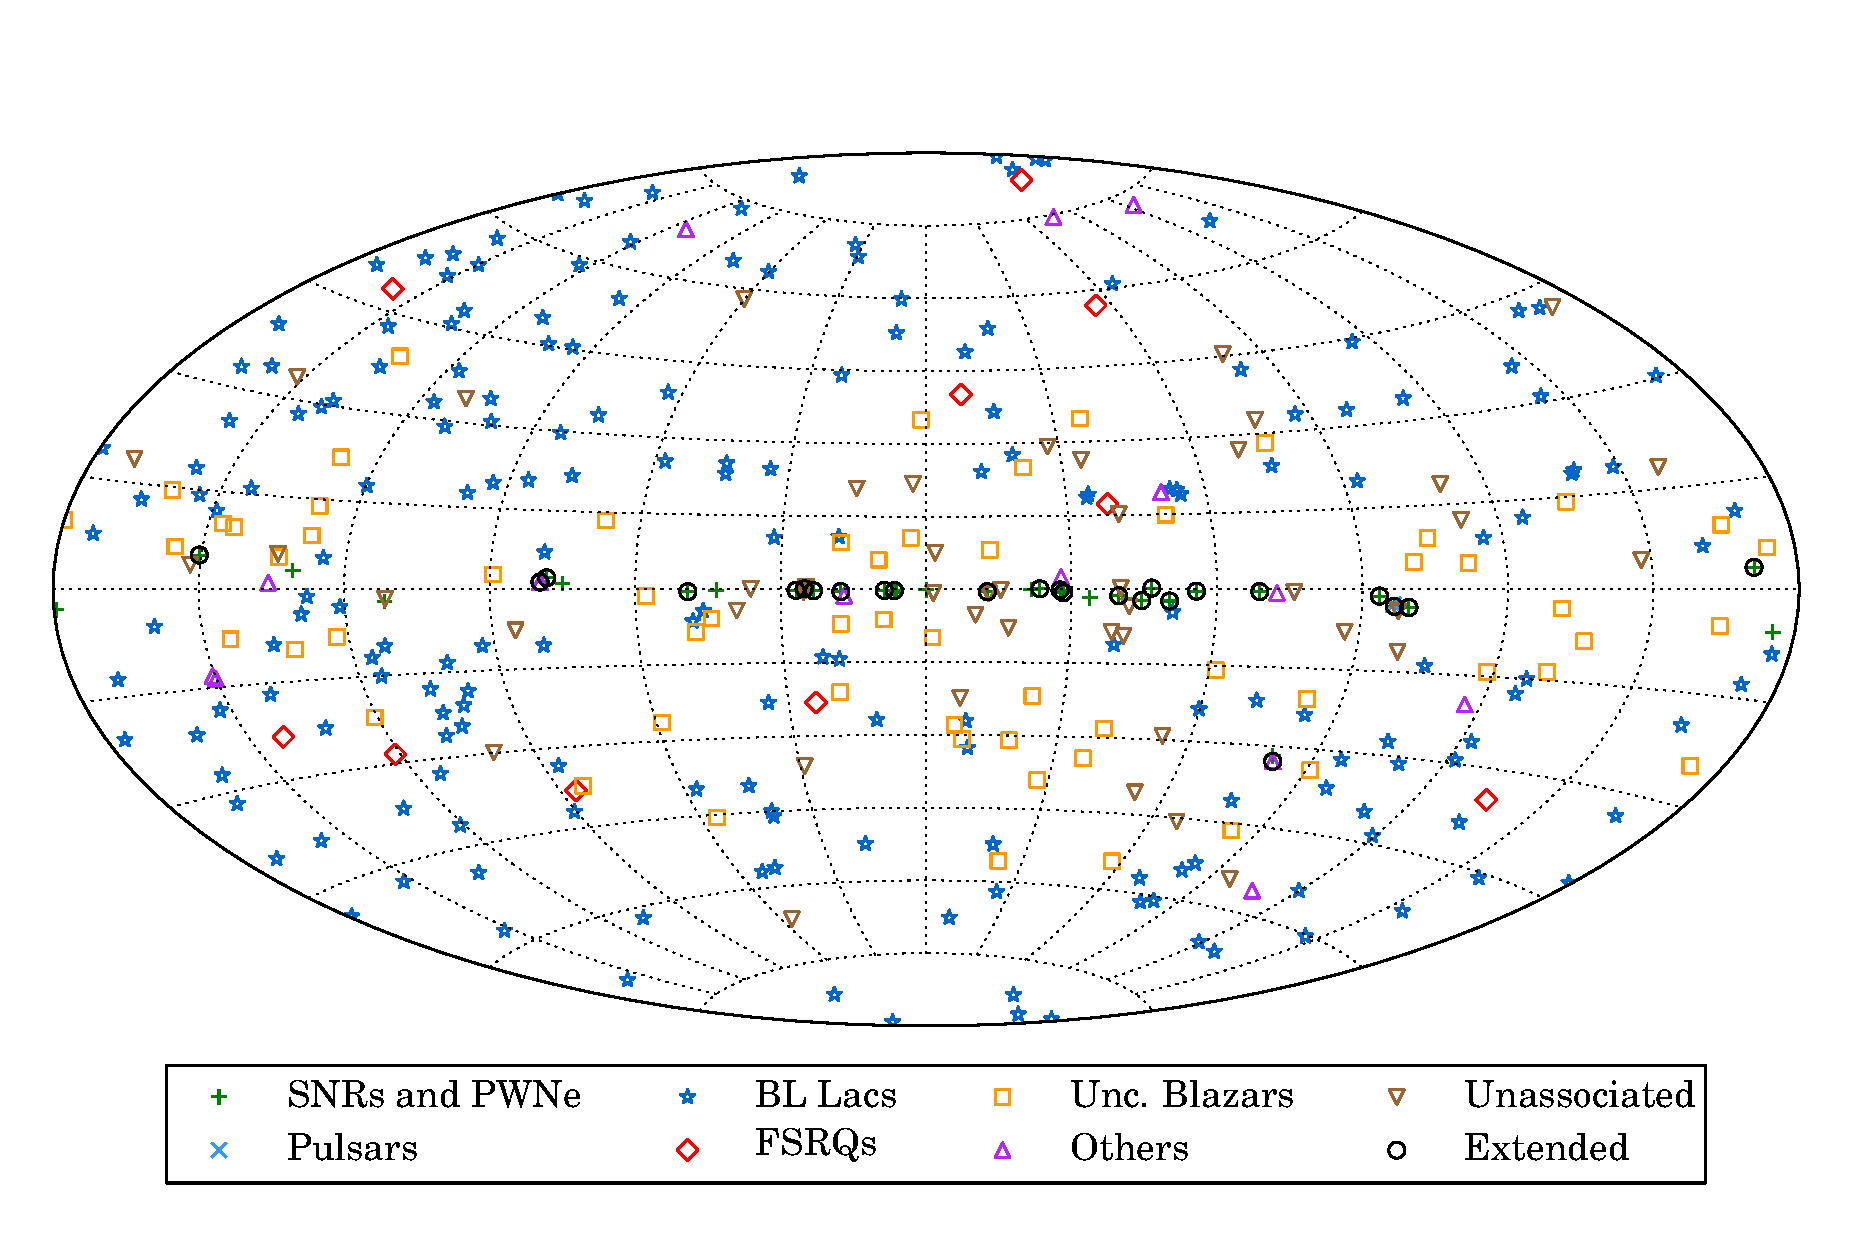
\includegraphics[width=\textwidth]{Figures/all-sky_assoc.eps} 
	\caption{Sky map, in Galactic coordinates and Hammer-Aitoff projection,
		showing the sources in the 2FHL catalog classified by their most likely association. 
		\label{fig:all_sky}}
\end{figure*}
The 2FHL catalog \footnote{FITS catalog can be found at \url{http://fermi.gsfc.nasa.gov/ssc/data/access/lat/2FHL/}} includes 360 sources detected over the whole sky, each with a likelihood test statistic of ${\rm TS}\geq 25$ and number of associated photons, $N_{\rm pred}\geq 3$. 
The source association procedure (detailed in \cite{2FHL}) finds that 75\% of the sources in the catalog (274 sources) are extragalactic\footnote{This includes N~157B, an extragalactic \pwn{}.}, 11\% (38 sources) are of Galactic nature, and 13\% (48 sources) are unassociated (or associated with a TeV source of unknown nature). The unassociated sources are divided between 23 sources located at $|b|<10^{\circ}$, and 25 sources at $|b|\geq 10^{\circ}$. Therefore the fraction of extragalactic sources in the sample is likely larger than 80\,\%. The number of 2FHL sources that have not been reported in 3FGL is 57, 47 of which have not been previously reported in any \lat{} catalog nor in the TeVCat\footnote{\url{http://tevcat.uchicago.edu/}} catalog of \tev{} detected sources, and are thus new $\gamma$-ray sources. % The results of the association procedures are summarized in Table~\ref{tab:class}.
 Figure~\ref{fig:all_sky} shows the location of 2FHL sources, color-coded according to their source class.\jamie{left out the assoc table}

%% Table listing the source classes and their numbers
\begin{deluxetable}{lcr}
\setlength{\tabcolsep}{0.04in}
\tablewidth{0pt}
\tabletypesize{\small}
\tablecaption{2FHL Source Classes \label{tab:class}}
\tablehead{
\colhead{Description} & 
\multicolumn{2}{c}{Associated} \\
& 
\colhead{Designator} &
\colhead{Number}
}
\startdata
Pulsar & psr & 1 \\
Pulsar wind nebula & pwn & 14 \\
Supernova remnant & snr & 16 \\
Supernova remnant / Pulsar wind nebula & spp & 4 \\
High-mass binary & hmb & 2 \\
Binary & bin & 1 \\
Star-forming region & sfr & 1 \\
BL Lac type of blazar & bll & 180 \\
BL Lac type of blazar with prominent galaxy emission & bll-g & 13 \\
FSRQ type of blazar & fsrq & 10 \\
Non-blazar active galaxy & agn & 2 \\ 
Radio galaxy & rdg & 4 \\
Radio galaxy / BL Lac  & rdg/bll & 2 \\
Blazar candidate of uncertain type I & bcu I & 7 \\
Blazar candidate of uncertain type II & bcu II & 34 \\ 
Blazar candidate of uncertain type III & bcu III & 19 \\  
Normal galaxy (or part) & gal & 1 \\
Galaxy cluster & galclu & 1 \\
Total associated & \nodata & 312 \\
%\hline
Unassociated & \nodata & 48 \\ 
\hline
Total in 2FHL & \nodata & 360 \\ 

\enddata
\tablecomments{The designation `spp' indicates potential association with SNR or PWN.
The `bcu I', `bcu II', and `bcu III' classes are derived from 3LAC  and describe the increasing lack of multiwavelength information to classify  the source as a blazar \citep[see ][for more details]{3LAC}. The designation `bll-g' is adapted from the BZCAT \citep{bzcat5} and indicates a blazar whose SED has a significant contribution from the host galaxy.}
\end{deluxetable}



%%%%%%%%%%%%%%%%%%%%%%%%%%%%%%%%%%%%%%%%%%%%%%%%%%%%%%%%%%%%%%%%
%
%         General Results
%
%%%%%%%%%%%%%%%%%%%%%%%%%%%%%%%%%%%%%%%%%%%%%%%%%%%%%%%%%%%%%%%%
\subsection{General Characteristics of 2FHL Sources}\label{2fhl:General}

The 2FHL sources have $>$ 50\,GeV fluxes ranging from
$\sim$$8\times 10^{-12}$~ph~cm$^{-2}$~s$^{-1}$ to $\sim$$1.3\times 10^{-9}$~ph~cm$^{-2}$~s$^{-1}$
with a median flux of  $2.0\times 10^{-11}$~ph~cm$^{-2}$~s$^{-1}$
and a median spectral index of 2.83. The index uncertainty increases rapidly with the spectral index (\eg{} the uncertainty is about
$\pm 0.5$ for sources with $\Gamma=2$ whereas it is 
$\pm 2$ for sources with $\Gamma=5$).
Half of the sources are localized to better than
1.7$'$ radius at 68\,\% confidence. 
\jamie{don't include flux vs index stuff}
%Figure~\ref{fig:index_vs_flux} plots the spectral index versus the photon flux for sources associated with extragalactic sources or located at \blot (the extragalactic sample), Galactic sources, and unassociated sources. Figure~\ref{fig:index_vs_flux} shows that there is no visible dependence of the sensitivity (i.e. minimum dethighlighting that the sensitivity for source detection becomes { worse} in the plane of the Galaxy.} 
The distributions of spectral indices and the highest photon energy reported in Figure~\ref{fig:hist_index} show that extragalactic sources tend to have larger photon indices (median of 3.13) than Galactic sources (median of 2.10).   Because of the harder spectra, Galactic sources tend to have higher-energy HEPs than those of extragalactic sources
as shown as well in Figure~\ref{fig:hist_index}.
It is interesting to note that unassociated sources have a median index of 2.22 (2.00 for  sources at \blat and 2.96 for those at \blot), showing that a fraction (see Chapter \ref{2fhl:GalPop}) of unassociated sources are likely of Galactic origin. 

Building a spectral energy distribution (SED) represents a powerful way to discriminate or infer the nature of a source. By combining the spectral data from the 3FGL, 1FHL, and 2FHL catalogs, it becomes possible to measure the SEDs
of sources over four decades in energy. Although these catalogs rely on different exposures and  most $\gamma$-ray sources are variable, these data allow us to characterize the high-energy peak of their broadband SEDs. The SEDs of a few notable sources will be shown in the next sections.

%%%%%%%%%%%%%%%%%%%%%%%%%%%%%%%%%%%%%%%%%%%%%%%%%%%%%%%%%%%%%%%%
%
%         Galactic Science
%
%%%%%%%%%%%%%%%%%%%%%%%%%%%%%%%%%%%%%%%%%%%%%%%%%%%%%%%%%%%%%%%%

\subsection{The 2FHL Galactic Source Population}\label{2fhl:GalPop}


The narrow PSF core (about $0.1^{\circ}$) and moderate Galactic diffuse emission (in comparison with the $>100$\,MeV band) allows the LAT to characterize and study well the emission of sources in the plane of our Galaxy above 50\,GeV. Within $|b|<10^{\circ}$, \lat{} has detected 103 sources.
Of those, 38 sources are associated with Galactic sources, 42 with blazars, 14 are unassociated and 9 are associated with other $\gamma$-ray sources
whose origin is not known (see below).
Figure~\ref{fig:gp1} shows cut-outs of the Galactic plane with all detected sources labeled.

\begin{figure*}[!ht]
    \begin{centering}
        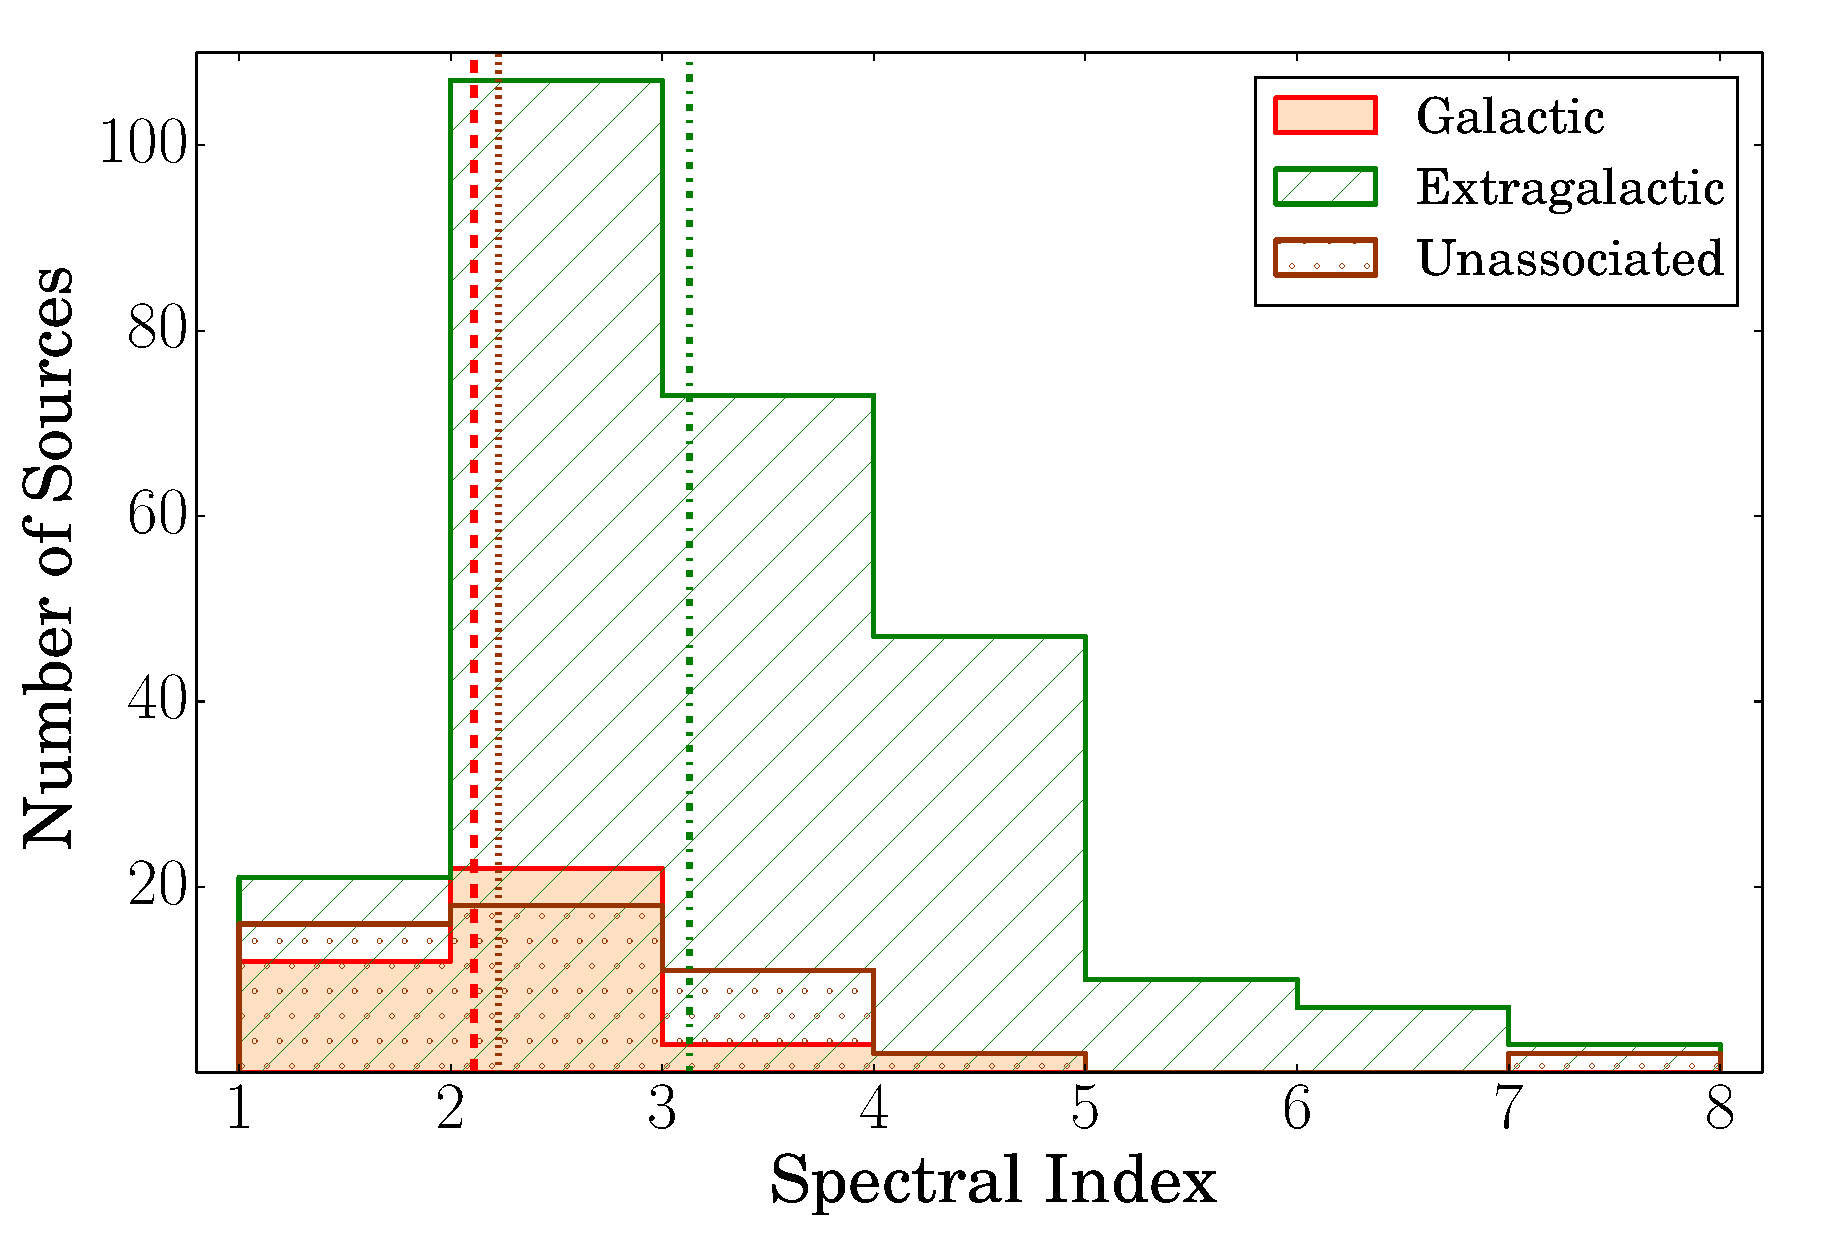
\includegraphics[width=0.9\columnwidth]{Figures/hist_index-new.eps}
         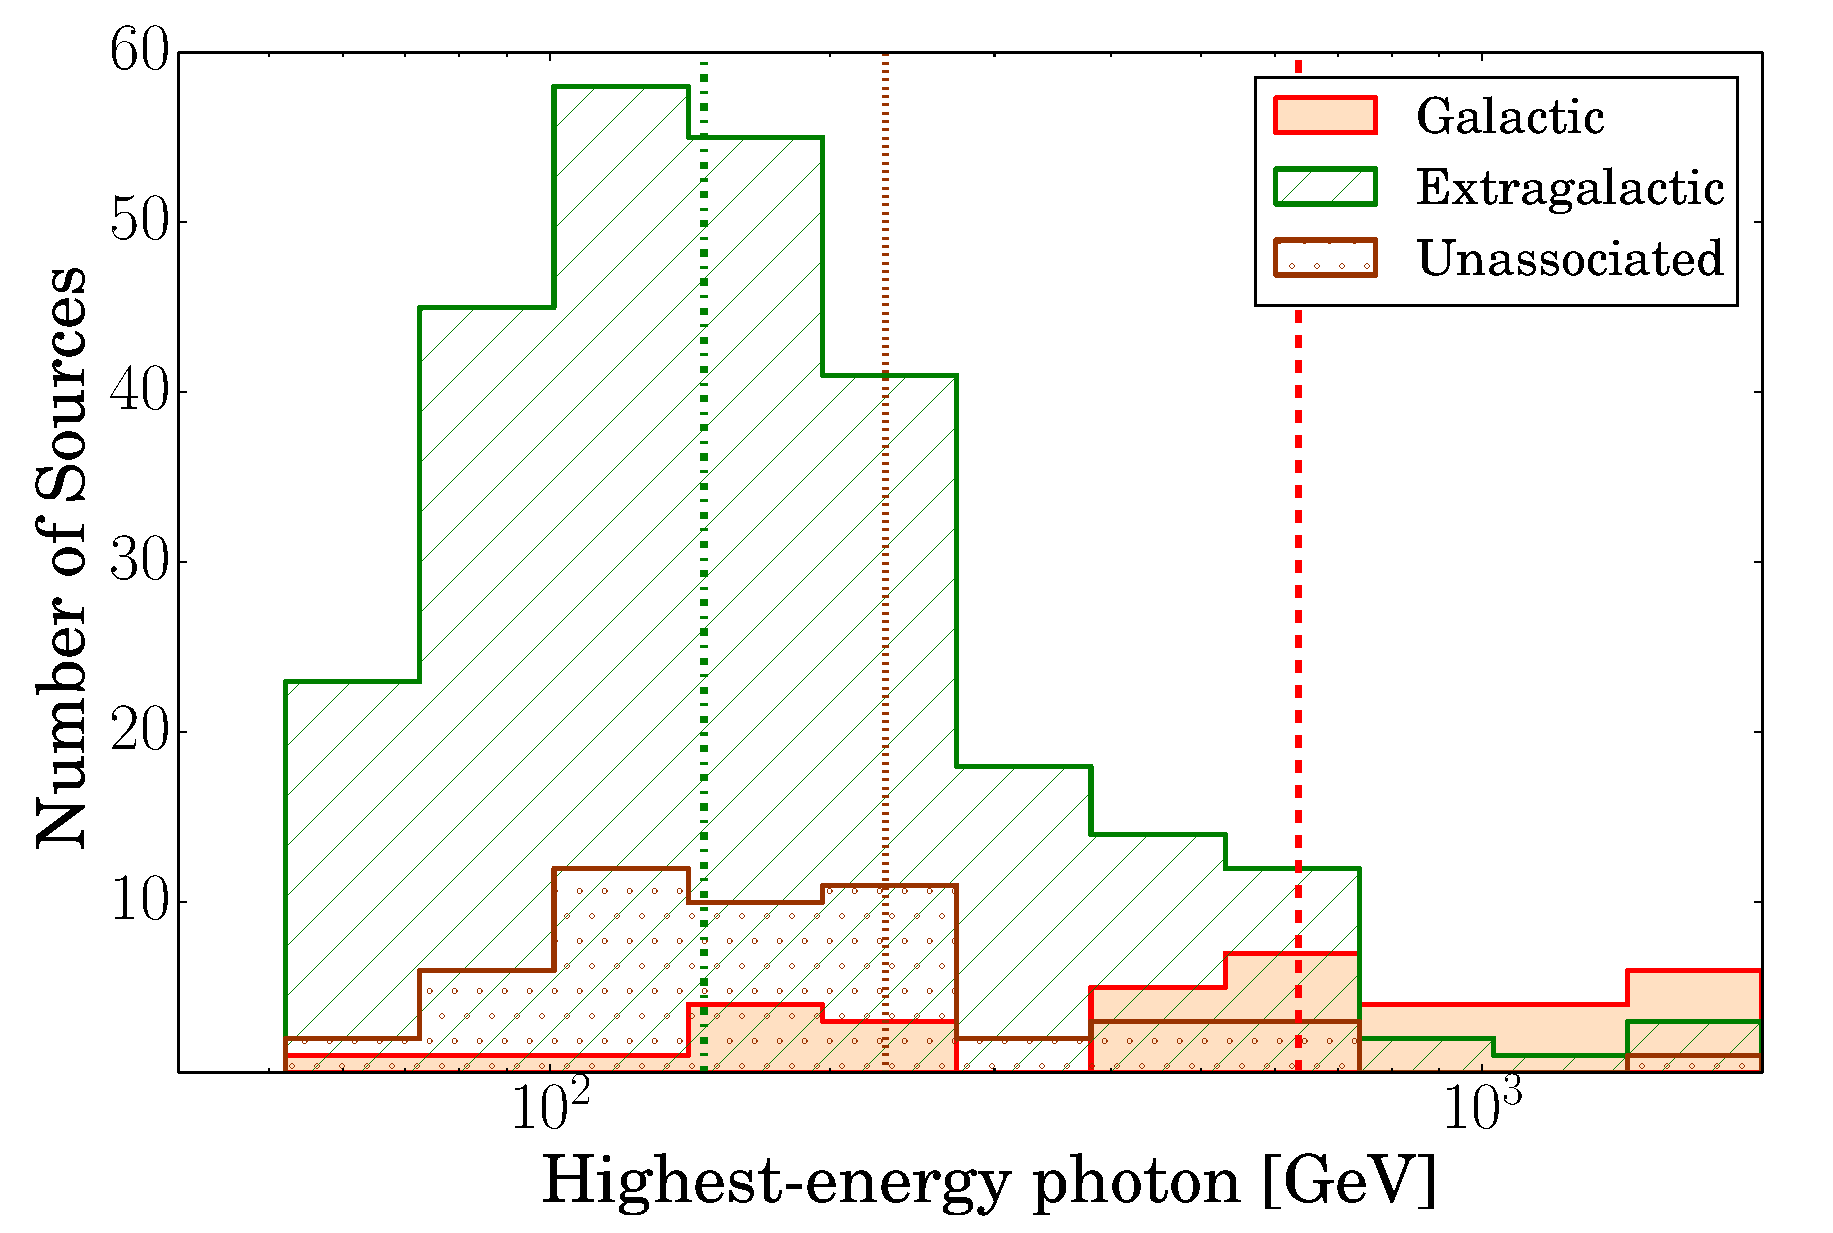
\includegraphics[width=0.9\columnwidth]{Figures/hist_hep-new.eps} 
        \caption{Distribution of the spectral indices ({\it top panel}) and highest photon energy ({\it bottom panel}) of the Galactic sources (orange), extragalactic sources (green slash), and unassociated sources (brown dotted). The medians of the distributions are plotted with dashed, dash-dotted, and dotted vertical lines, respectively. Both plots show that a distinct population of hard-spectrum sources is of Galactic origin.
            \label{fig:hist_index}}
    \end{centering}
\end{figure*}

Among the 38 Galactic sources, 16 are spatially coincident with SNRs, 13 are coincident with PWNe, 4 are associated with PWN/SNR complexes
and the other 5 sources are X-ray binaries (3), one pulsar (PSR~J0835$-$4510)
and the Cygnus Cocoon.
It is clear that the majority of Galactic sources detected above 50\,GeV
are associated with objects at the final stage of stellar evolution.

\begin{figure*}[!ht]
    \begin{center}
        \begin{tabular}{ll}
            % original scale=0.4
                    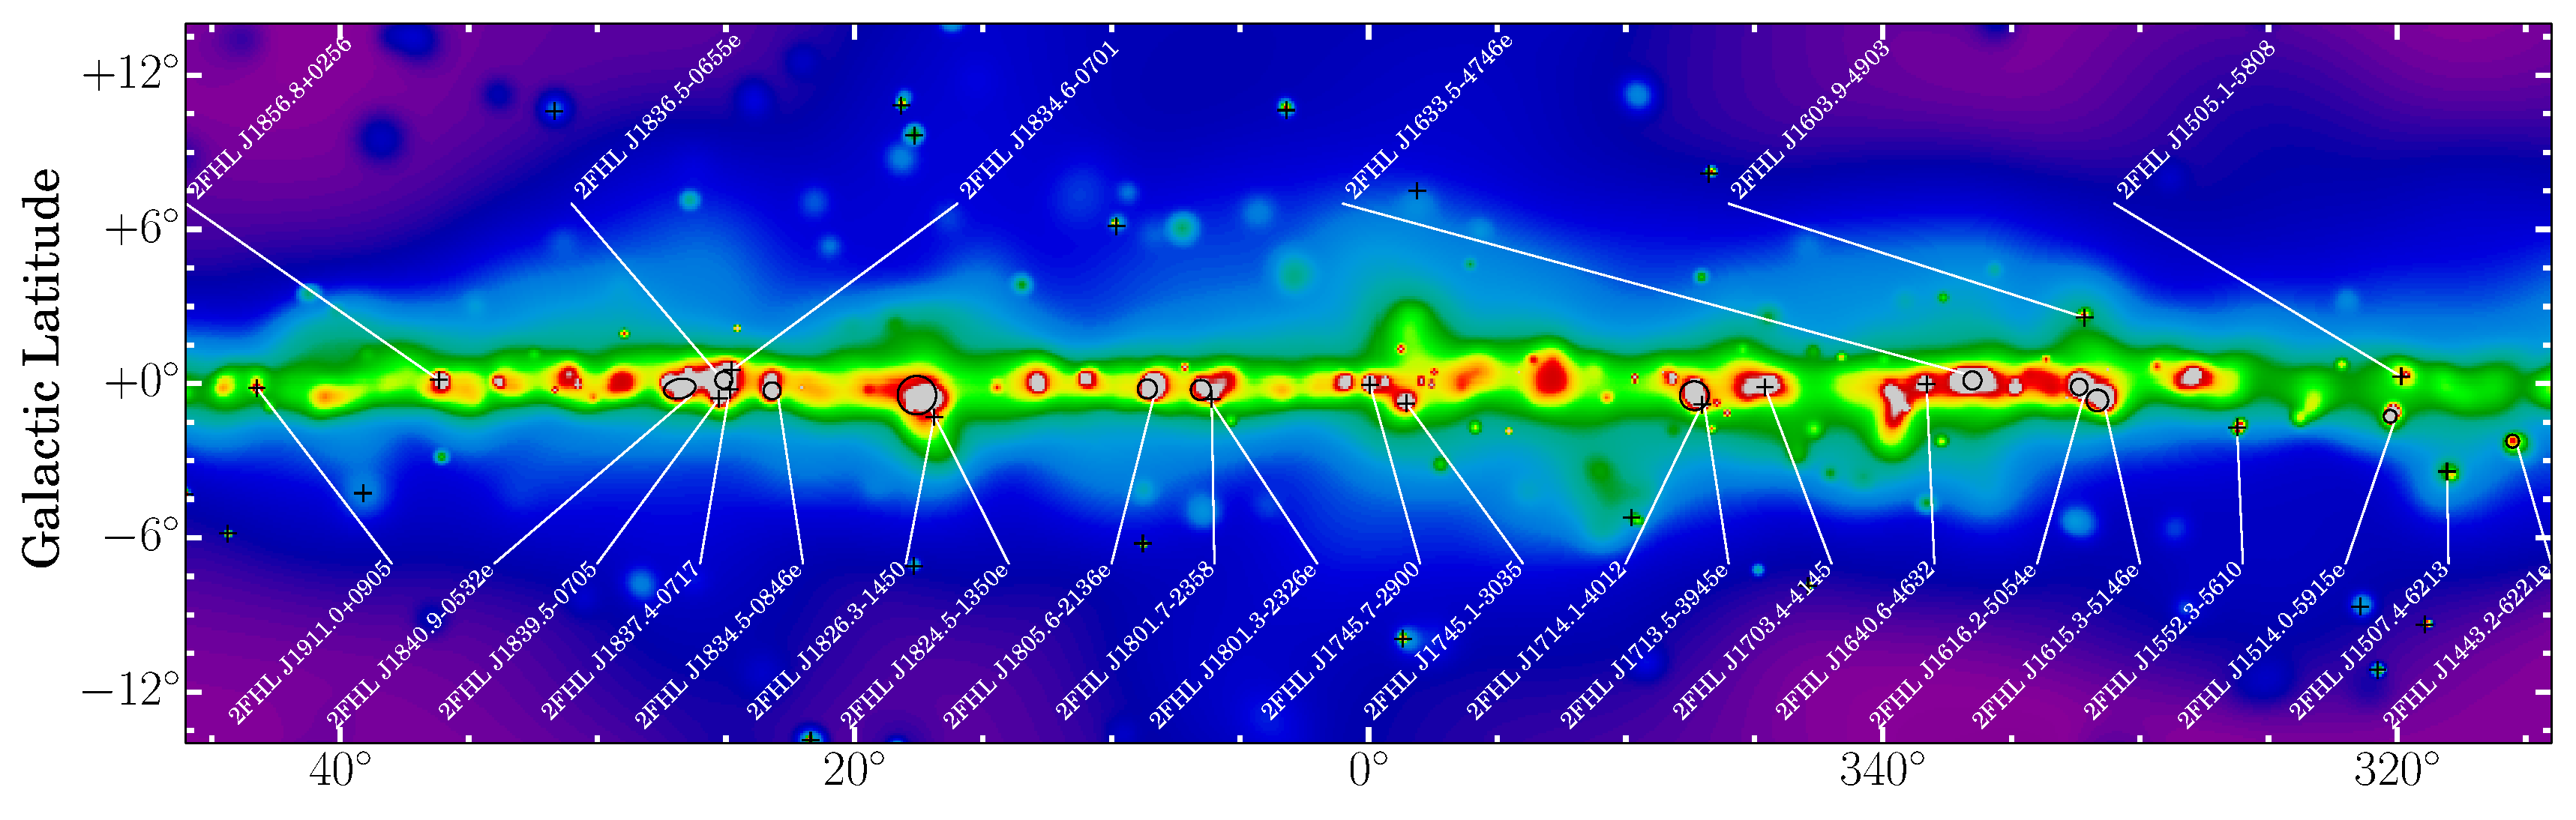
\includegraphics[angle=90,scale=.3]{Figures/Galactic_plane_CAR_1of4_sqrt_spectral_2FHL.eps}&
                    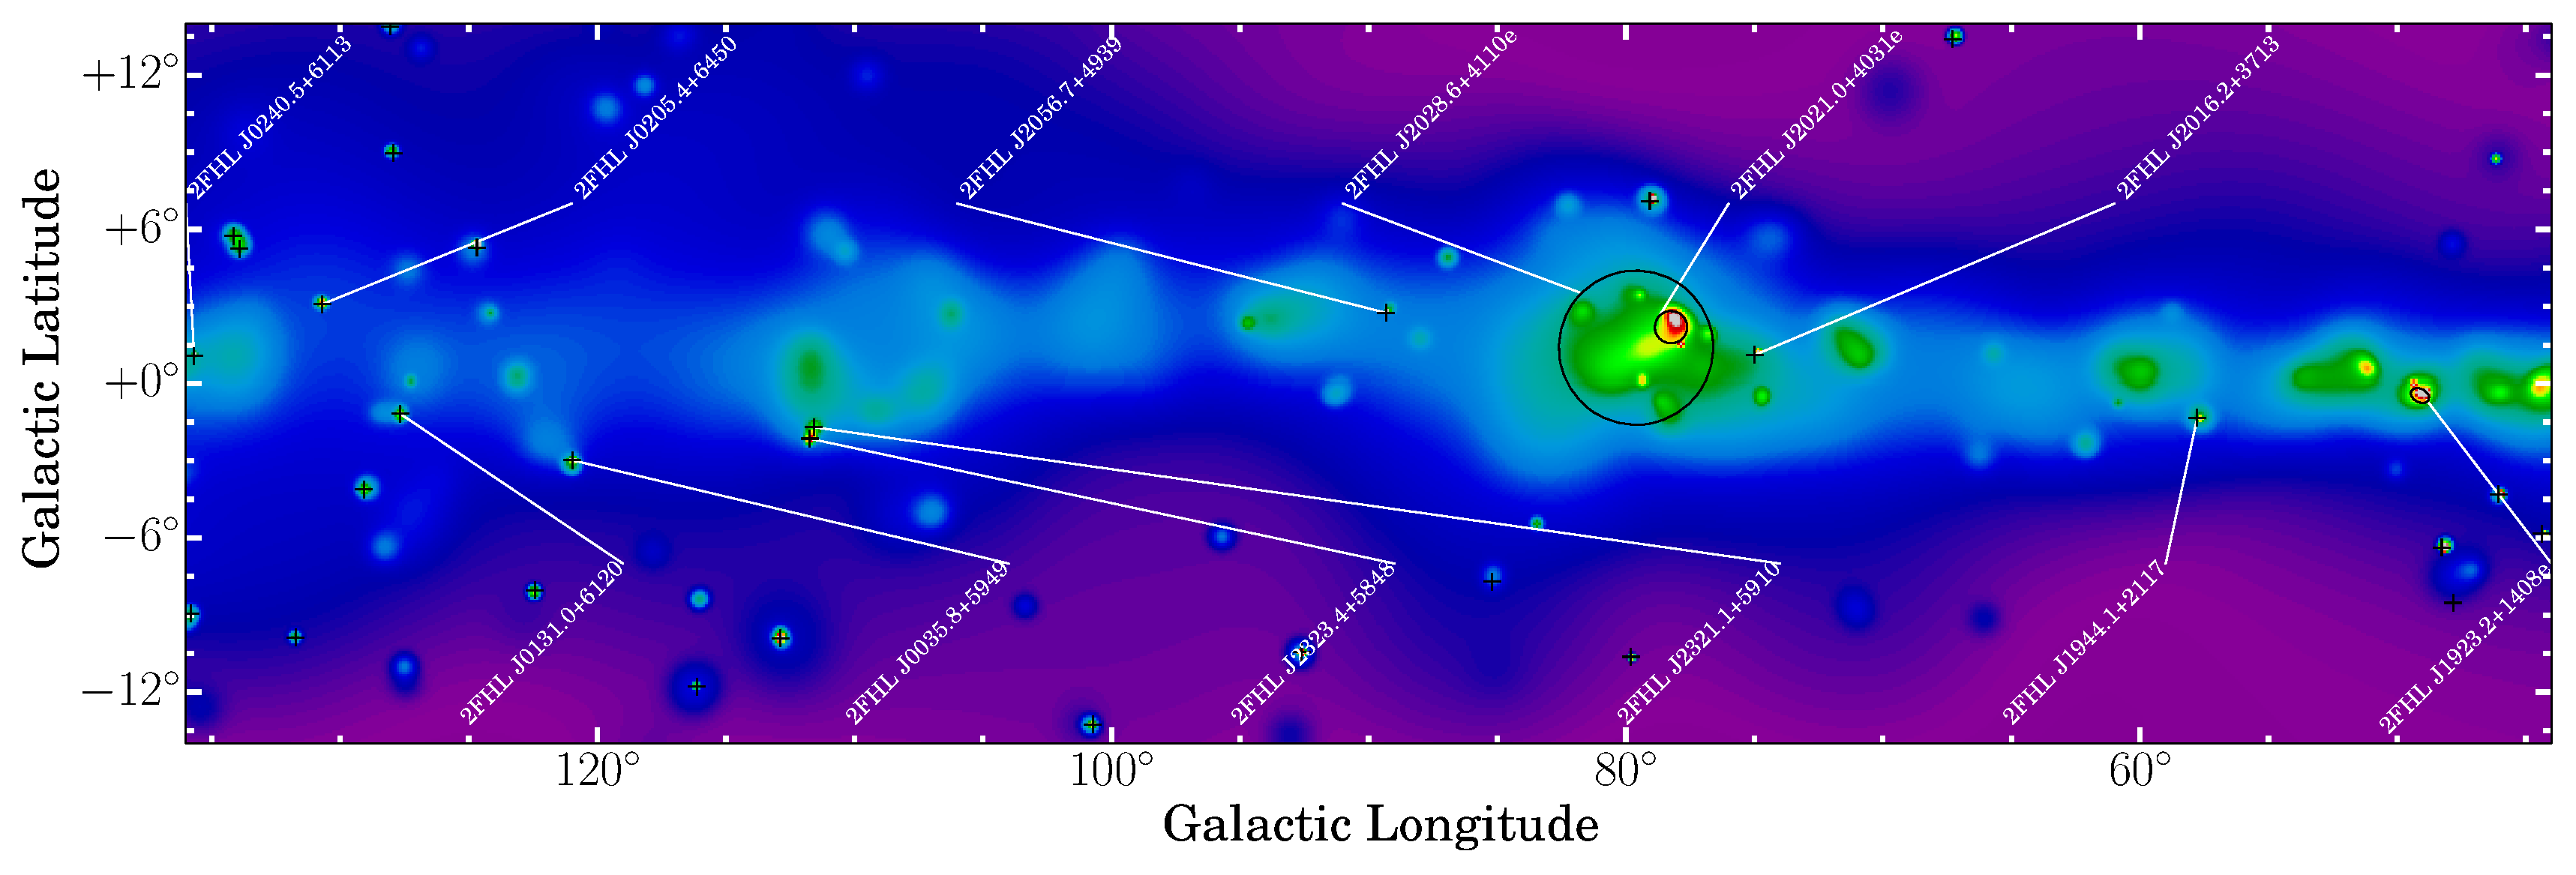
\includegraphics[angle=90,scale=.3]{Figures/Galactic_plane_CAR_2of4_sqrt_spectral_2FHL.eps}\\
            %\includegraphics[angle=90,scale=.3]{f5a.eps}&
            %\includegraphics[angle=90,scale=.3]{f5b.eps}\\
            
            
        \end{tabular}
    \end{center}
    \caption{Adaptively smoothed count map showing the whole Galactic plane $0^{\circ}\leq l\leq 360^{\circ}$ at Galactic latitudes $-14^{\circ} \leq b\leq 14^{\circ}$ divided in four  panels. The panels are centered at $l=0^{\circ}$, $90^{\circ}$, $180^{\circ}$ and $270^{\circ}$, respectively. Detected point sources are marked with a cross whereas extended sources are indicated with  their extensions. Only sources located at $-4^{\circ} \leq b\leq 4^{\circ}$ are explicitly named, plus the Crab Nebula.
        \label{fig:gp1}}
\end{figure*}


\begin{figure*}[!ht]
    \begin{center}
        \begin{tabular}{ll}
                    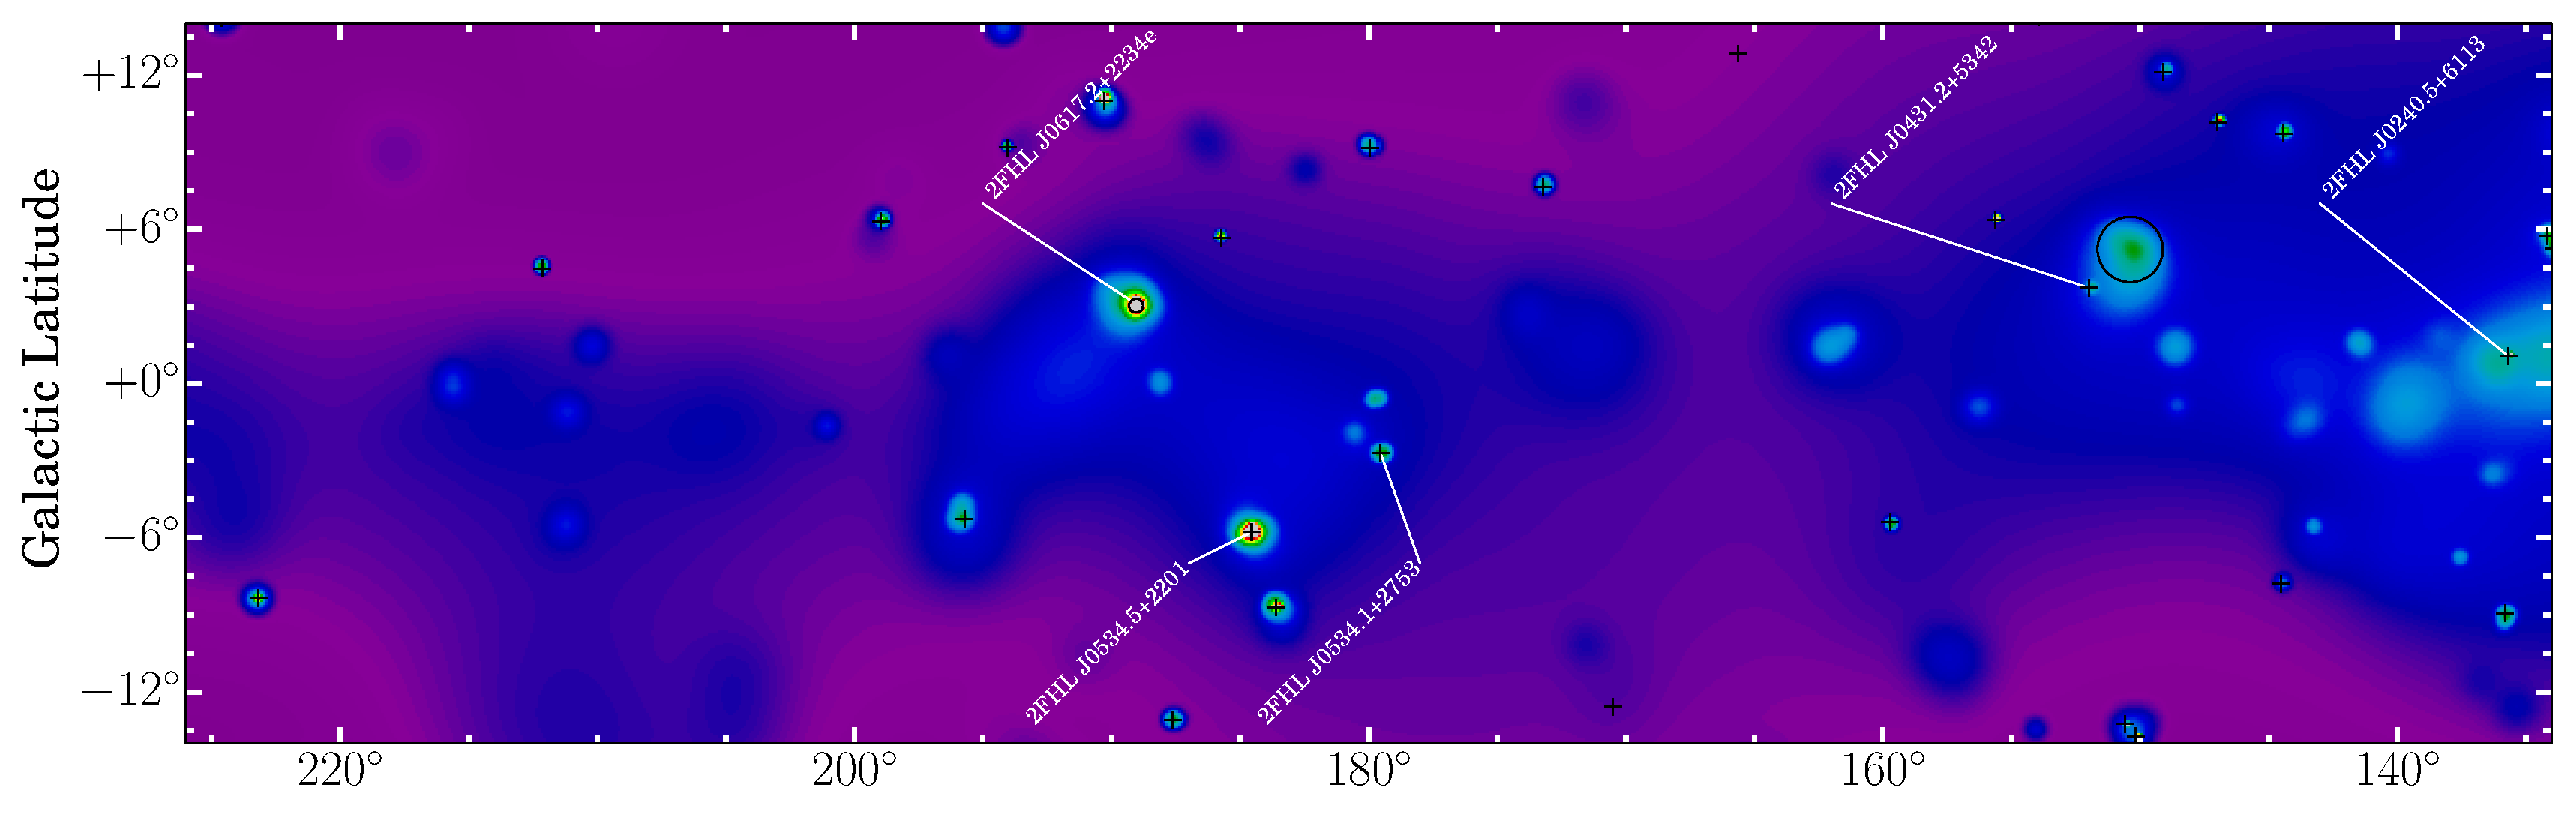
\includegraphics[angle=90,scale=.3]{Figures/Galactic_plane_CAR_3of4_sqrt_spectral_2FHL.eps}&
                    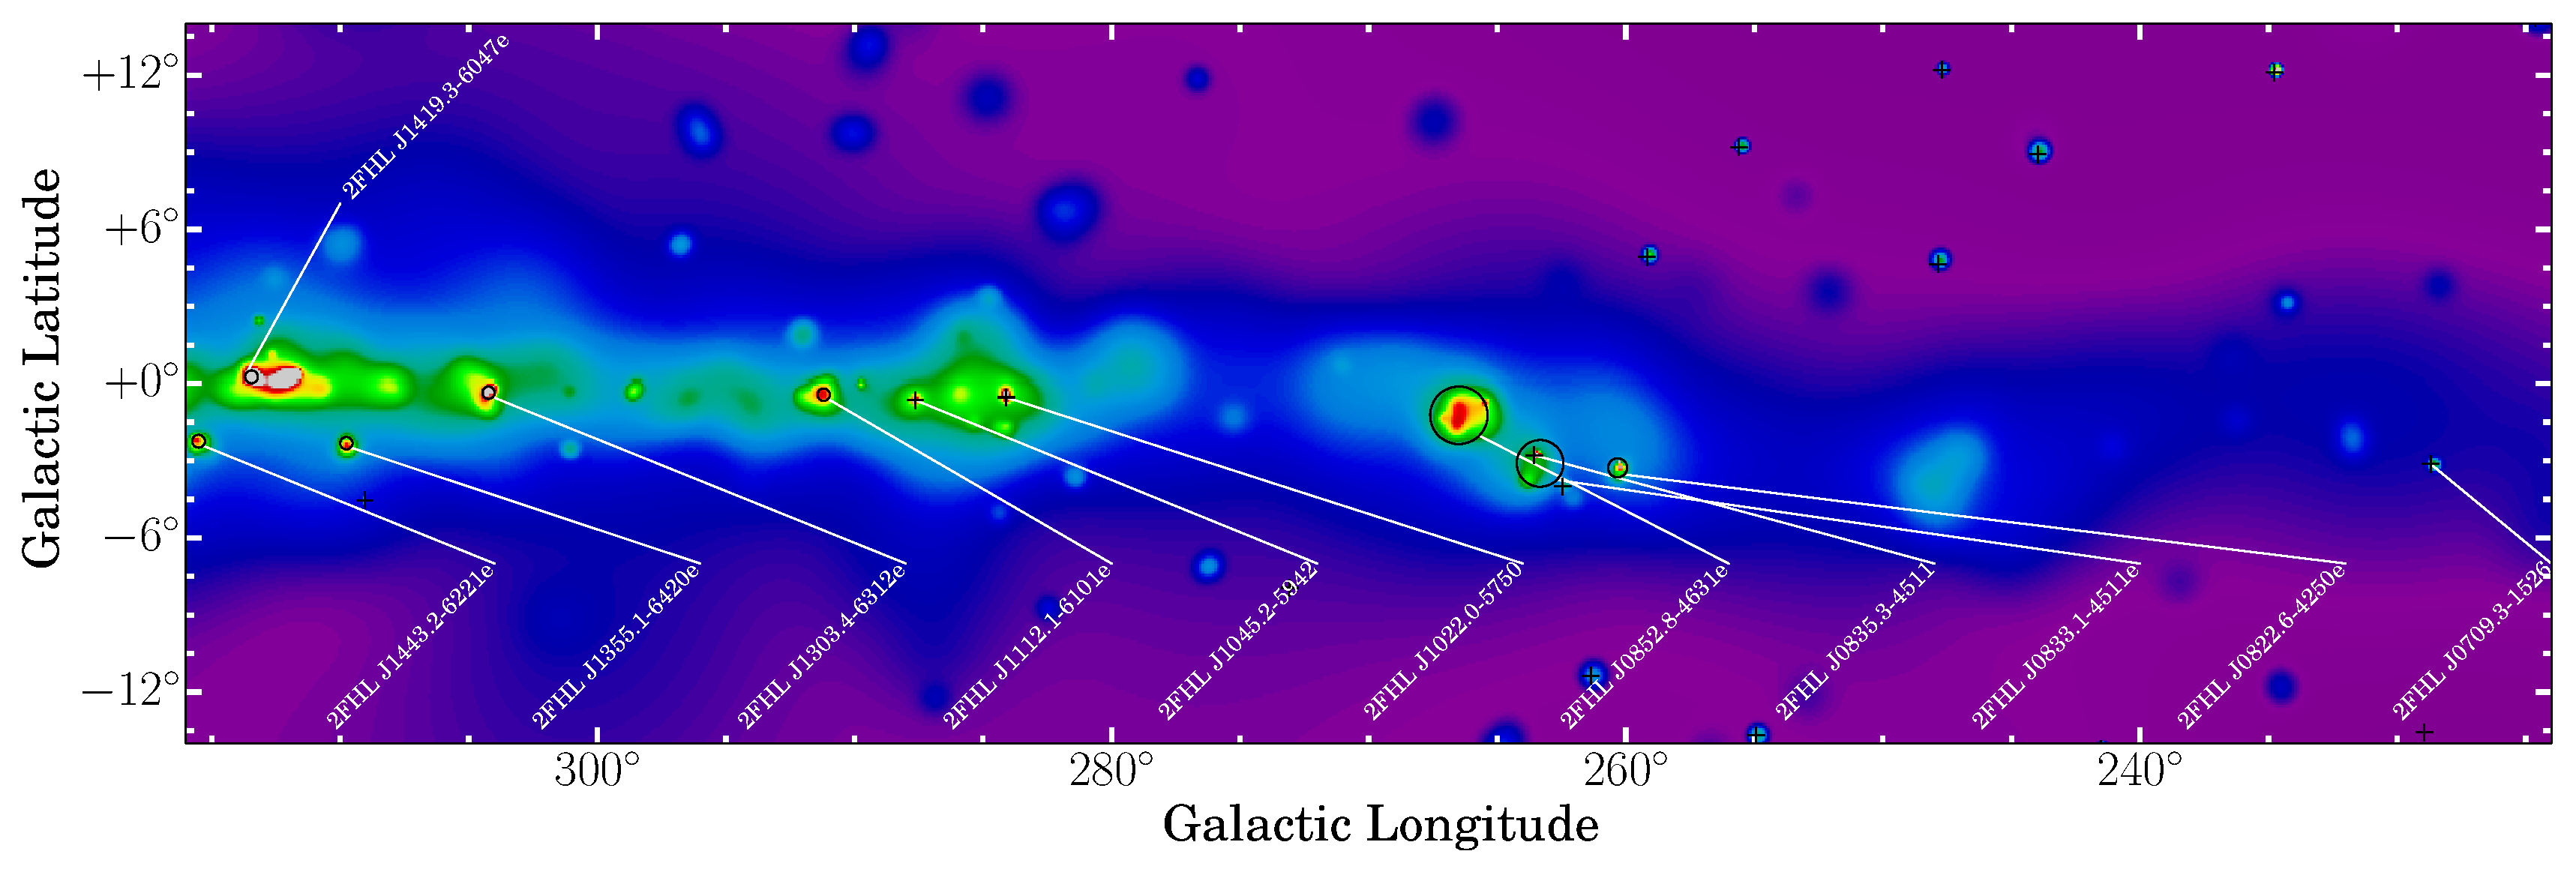
\includegraphics[angle=90,scale=.3]{Figures/Galactic_plane_CAR_4of4_sqrt_spectral_2FHL.eps}\\
            %\includegraphics[angle=90,scale=.3]{f5c.eps}&
            %\includegraphics[angle=90,scale=.3]{f5d.eps}\\
            
        \end{tabular}
    \end{center}
    \begin{flushleft}
        {Fig.~\ref{fig:gp1}.}---  continued
    \end{flushleft}
\end{figure*}

Galactic sources display on average hard spectra, which is a sign
of efficient particle acceleration. Roughly 55\% of all Galactic
sources have a spectral index lower than 2.2. For comparison, only 14\% of the { 2FHL} blazars
display such hard spectra. %With the exception of Eta Carinae (2FHL J1045.2-5942), all hard Galactic sources belong to either the PWN class (12 sources) or the SNR class (8 sources).
A sizable fraction (approximately 25\%, 
see Figure~\ref{fig:hist_index}, upper panel)
of Galactic sources has a photon
index harder than 2, implying a high-energy SED peak in the TeV band.
Indeed, as the lower panel of Figure~\ref{fig:hist_index} shows,
\lat{} detects emission from many Galactic sources well beyond 500\,GeV.
%All these sources belong to either the PWN or SNR classes.
All PWNe detected by {\it Fermi} are found to be powered by young
and energetic pulsars \citep[age $\lesssim 30$\,kyr,][]{Acero13}.
While it is common for PWNe to show hard spectra, this is less
so for SNRs whose majority (about 85\,\%) display softer spectra
\citep{snrCat}. Hard-spectrum SNRs are typically young or 
mid-aged ($\lesssim$3--5\,kyr)
and might be difficult to find in radio surveys. Thus, Galactic surveys
at above 50\,GeV have the capability to detect new SNRs that
might have been previously missed.
Such an example is represented by the extended source 
2FHL J0431.2+5553e which is spatially coincident with a 
new SNR (SNR G150.3+4.5) recently reported by \cite{Gao14} (see Chapter \ref{chap:G150}).

Of the 14 sources at $|b|<10^{\circ}$ that do not have an
association, 7 have power-law indices harder than 2
which renders them  likely Galactic objects.
It is interesting to note that { 6 of these 7 objects} are offset from the plane of the Galaxy  by more than $4^{\circ}$. This is in marked contrast with the 
associated portion of the sample where only the Crab Nebula and the
newly discovered SNR G150.3+4.5 (out of 34 SNR/PWN systems) have such
a large offset. Thus it seems unlikely that all these unassociated sources
are SNR/PWN systems.

%%%%%%%%%%%%%%%%%%%%%%%%%%%%%%%%%%%%%%%%%%%%%%%%%%%%%%%%%%
%
% H E S S 
%
%%%%%%%%%%%%%%%%%%%%%%%%%%%%%%%%%%%%%%%%%%%%%%%%%%%%%%%%%%%

\subsection{Comparison with the H.E.S.S. Galactic Plane Survey}\label{2fhl:HESS}
The H.E.S.S array, with a field of view of about 5$^{\circ}$ and an angular resolution of approximately 0.12$^\circ$, has invested 2800\,hrs of exposure to survey  part\footnote{The H.E.S.S. Galactic plane survey extends between 283$^{\circ}<l<$59$^{\circ}$ and Galactic latitudes of $|b|<3.5^{\circ}$.} 
of the Galactic plane, reaching an average sensitivity of 2\,\% of the Crab Nebula flux (i.e. 4.5$\times10^{-13}$\,ph~cm$^{-2}$~s$^{-1}$) at $\geq$1\,TeV \citep{aharonian06_gps,carrigan2013}. Considering that the Crab Nebula spectrum is harder
in the 2FHL band than in the $>$1\,TeV band, we estimate that the average sensitivity of 2FHL in the same region of the H.E.S.S. survey is $\sim$3--4\,\% of the { 50\,GeV--2\,TeV Crab Nebula flux.} The slightly better sensitivity 
allows H.E.S.S. to detect 69 sources (as reported in the TeVCat), while
the LAT finds 36 objects in the same area. However, the comparable sensitivities of the two surveys allow the study of the  properties of the high-energy Galactic population.
%%%% USE following to convert the 2% >1TeV Crab nebula flux to
%%%%     2FHL flux
%%%%  4.5e-13*(pow(2.,-1.3)-pow(50./1000.,-1.3))/(pow(100.,-1.3)-pow(1.,-1.3))
%%%%
%%%%  The HESS Crab has an index of 2.3
%%%%  The Fermi Crab has index of 2.13 and flux 1.31e-9 ph/cm2/s
In the 2FHL catalog there is almost an equal number of SNRs and PWNe
in contrast to what is found in the  H.E.S.S. survey where the ratio
of PWNe to SNRs is 1.5 to 1. This might be because
the hardest PWNe and softest SNRs { are difficult to detect} respectively
in the $>$50\,GeV and $>$1\,TeV bands.


Of the 36 2FHL sources that fall within the footprint of 
the H.E.S.S. survey, 23 have already been detected
at TeV energies and are associated with known counterparts,
while 7 are undetected. The remaining 6 objects
(2FHL~J1022.0$-$5750, 2FHL~J1505.1$-$5808,  2FHL~J1507.4$-$6213, 2FHL~J1703.4$-$4145, 2FHL~J1745.1$-$3035 and  2FHL~J1856.8+0256)
are spatially coincident with TeV sources whose origin is not known.
All of them have hard spectral indices ($\Gamma<$2.2), but
it is interesting to note that 4 of them 
(2FHL~J1022.0$-$5750, 2FHL~J1505.1$-$5808, 2FHL~J1703.4$-$4145, and 2FHL~J1745.1$-$3035)
have $\Gamma<1.7$ (see also Figure~\ref{fig:gal_sed}).

We find that 2FHL~J1022.0$-$5750 is spatially compatible with
{ HESS~J1023$-$575, an extended TeV source \citep{westerlund2_hess11},
    whose emission might be due to a PWN powered by PSR~J1023$-$5746 \citep{Acero13}. }
%Westerlund 2 (TeV~J1023$-$5747), a massive star cluster already detected as an extended source at TeV energies \citep{westerlund2_hess11}.
2FHL~J1505.1$-$5808 is spatially coincident with the unidentified
object HESS~J1503$-$582, which has a size of 0.26$^{\circ}$ and a flux above 1\,TeV \citep{renaud08} compatible with the extrapolation of the 2FHL J1505.1$-$5808 spectrum.
Its spectrum, reminiscent of that of a PWN 
\citep[\eg{}, HESS~J1825$-$137,][]{grondin2011},
 is reported in Figure~\ref{fig:gal_sed}.


2FHL~J1507.4$-$6213 is spatially coincident with HESS~J1507$-$622, an extended source with a radius of 0.15$^{\circ}$ located  3.5$^{\circ}$ from the plane \citep{acero11}. The analysis of multiwavelength data showed that it is not possible to discriminate between a hadronic and leptonic origin of the emission, but that the latter scenario, if the emission is powered by a PWN, would require a pulsar generated in the explosion of a hyper-velocity star in order to reach the required distance from the plane \citep{domainko2012}.



The sources 2FHL~J1703.4$-$4145 and 2FHL~J1745.1$-$3035 are the hardest sources ($\Gamma<1.3$) among the six objects.
2FHL~J1703.4$-$4145 is spatially coincident with the bright radio emission
observed from the western side of the shell of SNR G344.7$-$001,
a nearby mid-aged  shell-type (age $\sim3000$\,yr and 8$'$ diameter) SNR \citep{giacani2011}. Both the 2FHL source and the SNR are spatially coincident
with the larger, elongated and unidentified HESS~J1702$-$420 \citep{aharonian08}.
It thus seems likely that  SNR G344.7$-$001 is the  counterpart
of  2FHL J1703.4$-$4145 and perhaps also of HESS~J1702$-$420.
The combined {\it Fermi}-H.E.S.S. spectrum of this source is reported in Figure~\ref{fig:gal_sed}.



2FHL~J1745.1$-$3035 is found to be spatially coincident with 
the extended source HESS~J1745$-$303, which may be comprised of
up to three different sources \citep{aharonian2008_j1745}. Indeed, the position of
2FHL~J1745.1$-$3035 is compatible  with the 'C' emission
region \citep[the second brightest region in the complex,][]{aharonian2008_j1745}.
However, the nature of this source is more complex, because
the 2FHL source is marginally brighter at 1\,TeV than the entire H.E.S.S. region and also has a harder spectrum (spectral index of 1.25$\pm0.38$ in 2FHL 
versus $2.17\pm 0.11$ as measured by H.E.S.S.).

Finally, 2FHL~J1856.8+0256 is coincident with HESS~J1857+026, an almost radially symmetric extended source  \citep{aharonian08_unid}, whose emission likely originates from a PWN powered by PSR~J1856+0245 \citep{rosseau2012}.

\begin{figure*}[ht]
    \begin{center}
       \hspace*{-1.5cm} \begin{tabular}{ll}
            \includegraphics[width=8cm]{Figures/{J0617.2+2234e_SED}.eps} &
            \includegraphics[width=8cm]{Figures/{J1419.3-6047e_SED}.eps}\\
            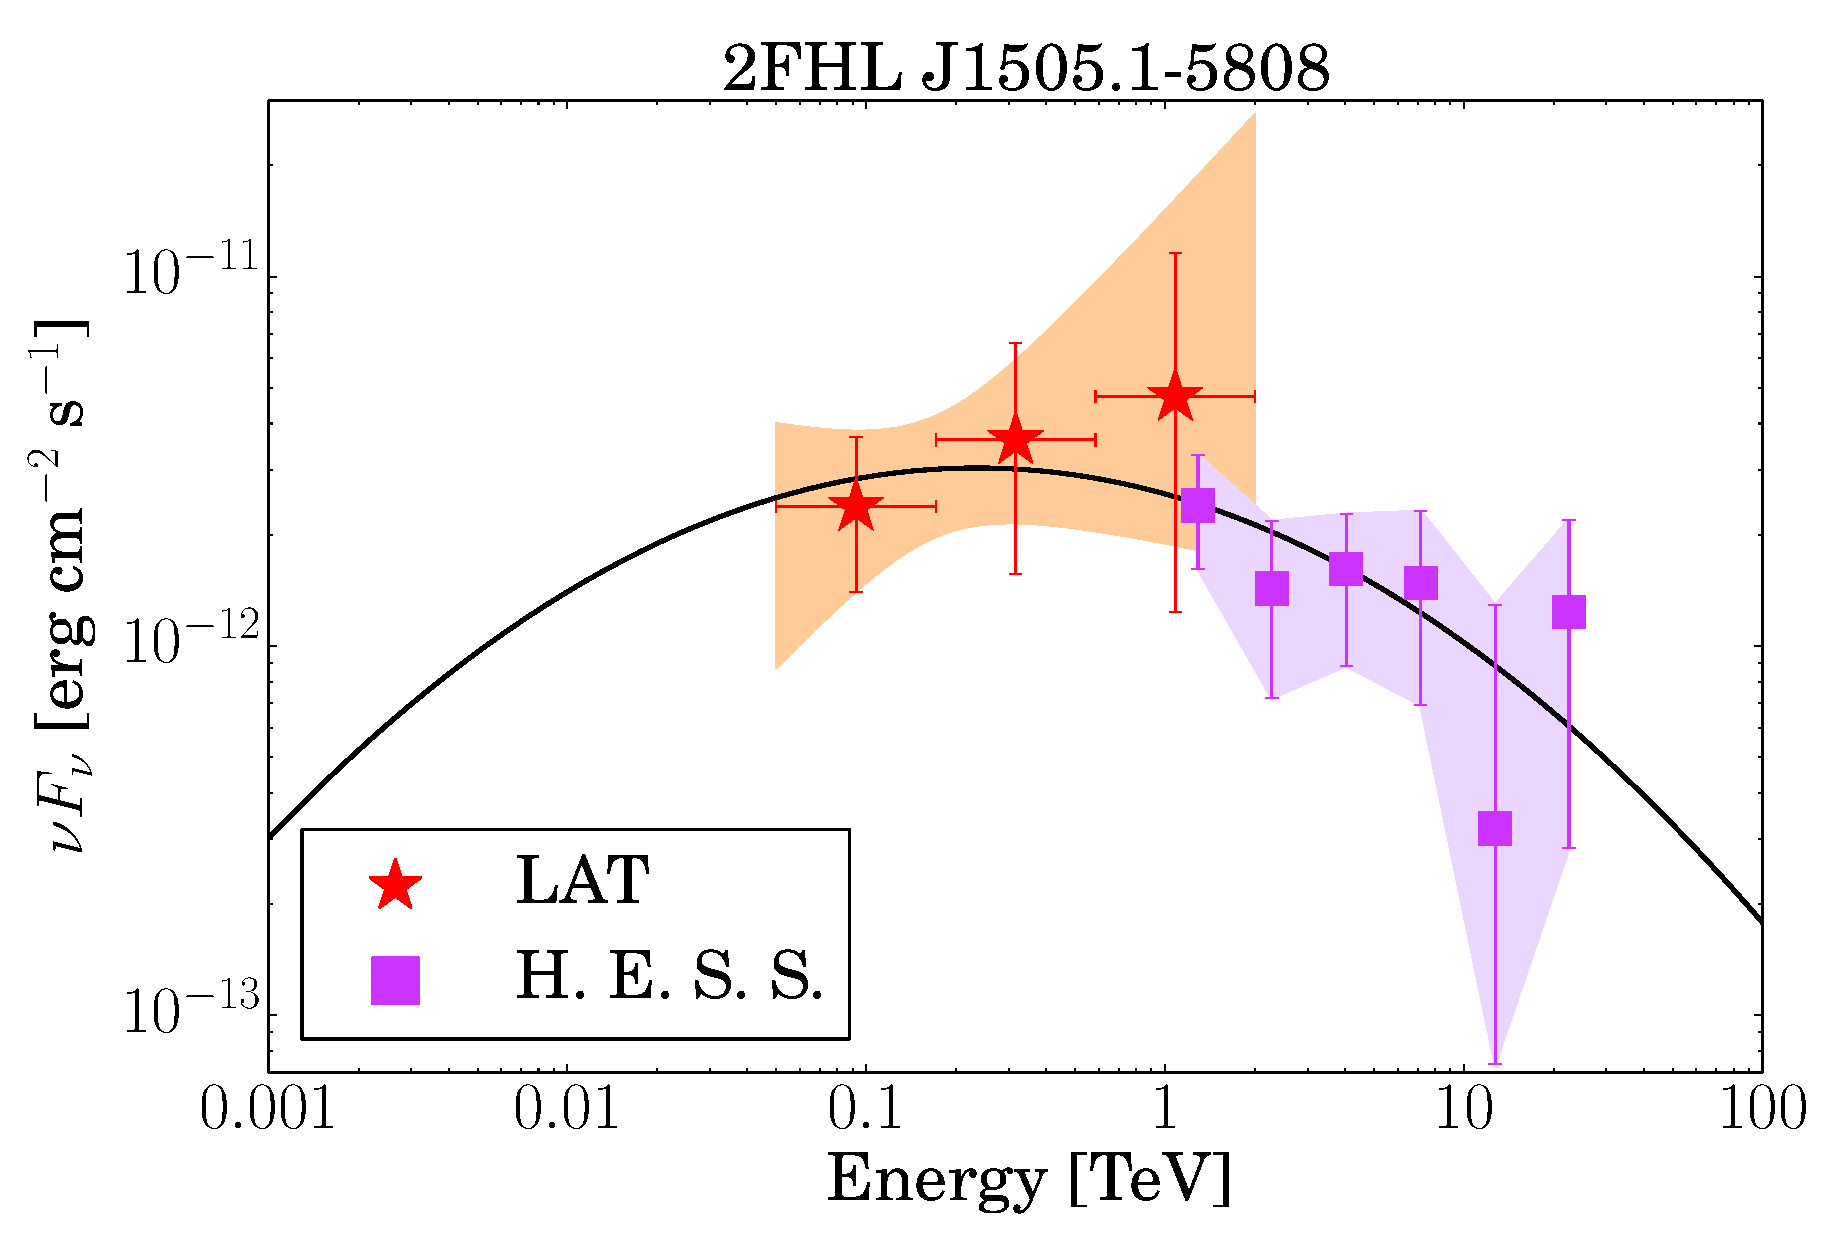
\includegraphics[width=8cm]{Figures/pgw_00682_SED.eps} &
            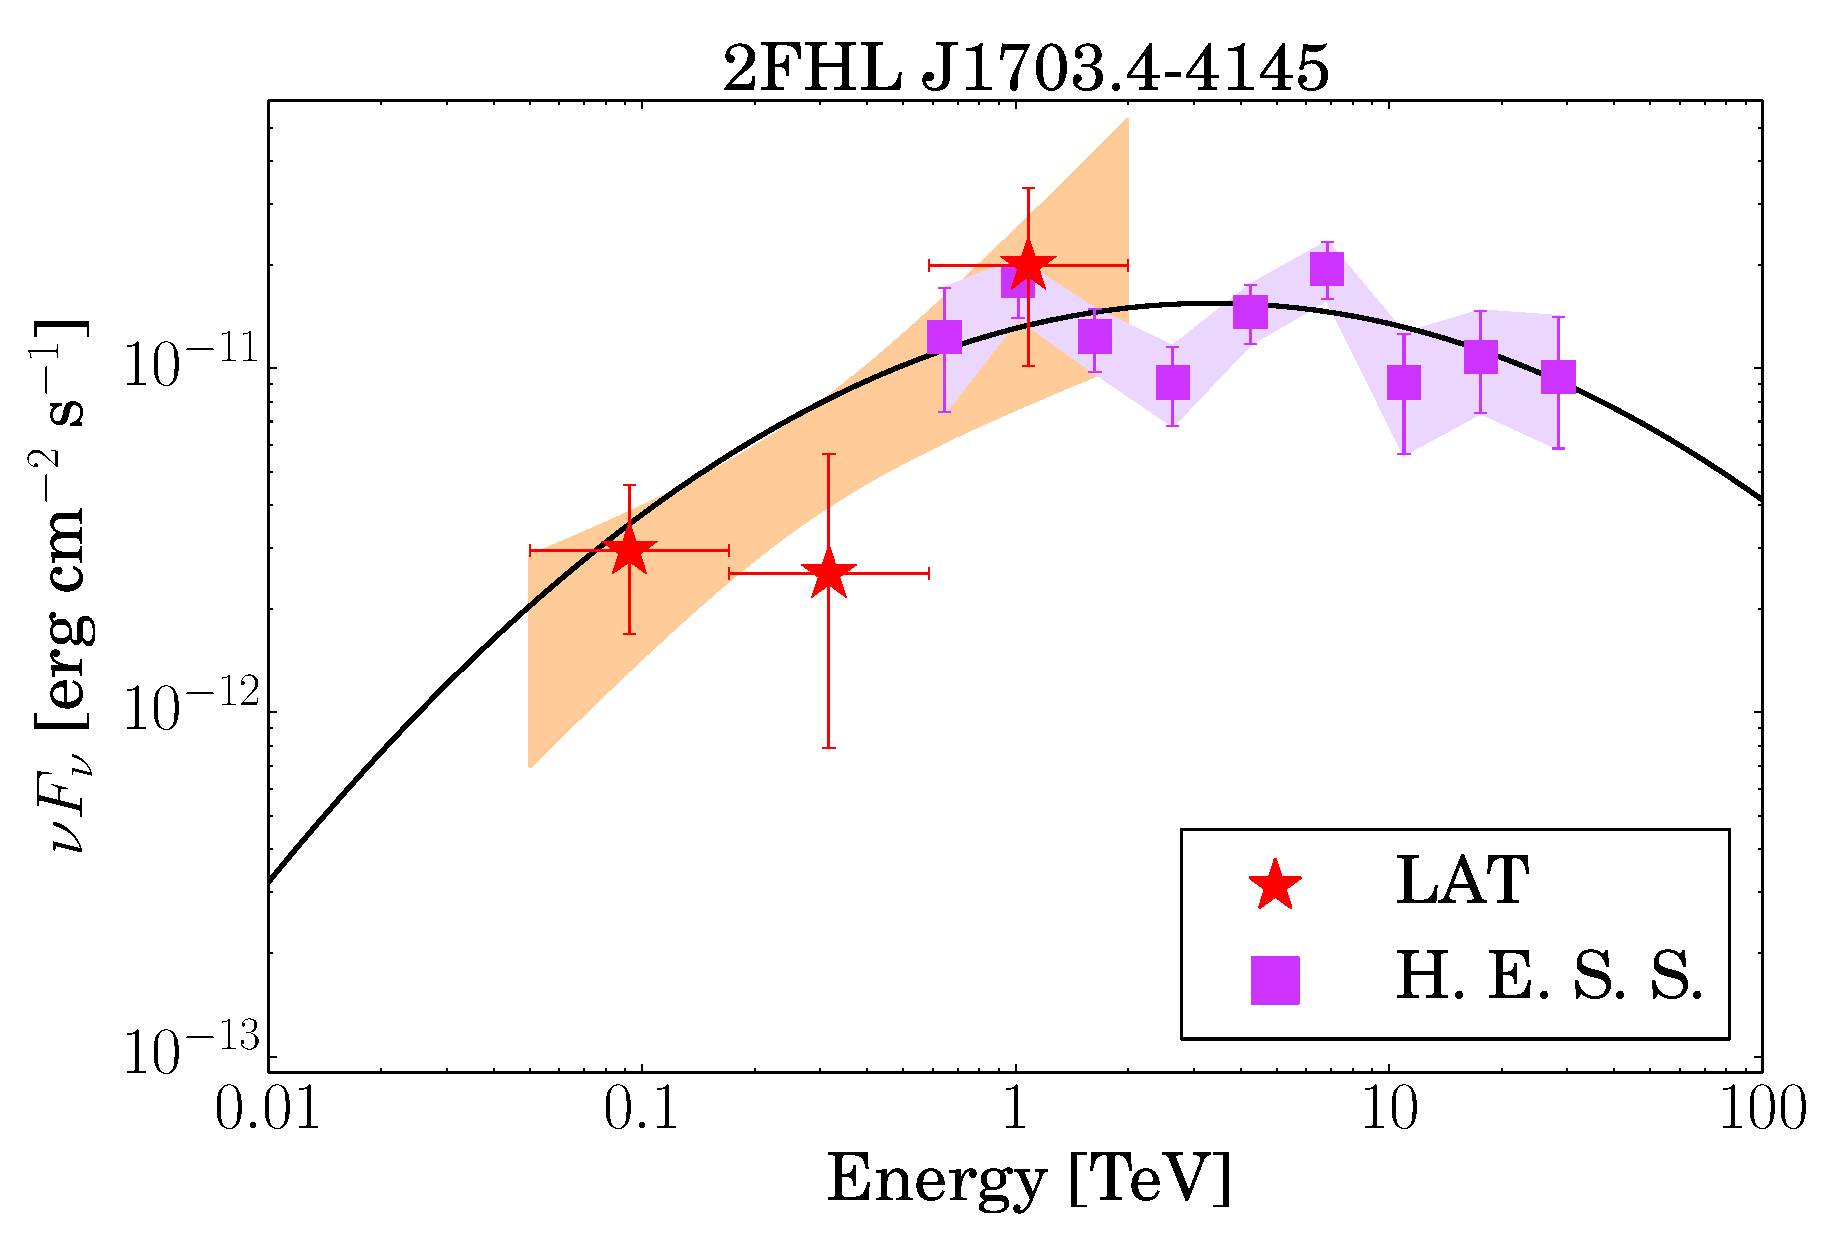
\includegraphics[width=8cm]{Figures/pgw_00110_SED.eps} \\
        \end{tabular}
    \end{center}
    \caption{
        \label{fig:gal_sed}Spectral energy distributions of four Galactic sources constructed by combining data from the 3FGL (green diamonds), 1FHL (blue circles), and 2FHL (red stars). We show the 3FGL extended source SNR IC~443 (\emph{top left}), the new 2FHL extended source PSR~J1420$-$6048 (\emph{top right}), and two ``dark accelerators'' detected by H.E.S.S. at TeV energies \citep[][purple squares]{carrigan2013} without a previous LAT counterpart:  { HESS~J1503$-$582} (\emph{bottom left}) and HESS~J1702$-$420 (\emph{bottom right}).}
\end{figure*}

%%%%%%%%%%%%%%%%%%%%%%%%%%%%%%%%%%%%%%%%%%%%%%%%%%%%%%%%%%%%%%%%%%%
%
%  Extended Source Results
%
%%%%%%%%%%%%%%%%%%%%%%%%%%%%%%%%%%%%%%%%%%%%%%%%%%%%%%%%%%%%%%%

\subsection{\label{2fhl:ESresults}Extended Source Results}


In total, 31 sources are modeled as spatially extended and input into the ML analysis: 25 listed in 3FGL, 5 sources detected in the {\tt pointlike} analysis (described in Chapter \ref{2fhl:3FGL_ES}) that were not { detected as extended at the time of} 3FGL, and one, SNR W41, reported  recently by both the H.E.S.S. and LAT teams \citep{HESSLATW41}. Names and properties of the extended sources  are provided in Tables \ref{tab:extended} and \ref{tab:new_extended}. 
Six extended sources, detected in 3FGL, were not detected in 2FHL: the SMC, S~147 ({the point source 2FHL~J0534.1+2753 was detected inside it}), the lobes of Centaurus A (although we detect its core as a point source, 2FHL J1325.6$-$4301), W~44, HB~21 and the Cygnus Loop.

We detect a weak source, 2FHL~J1714.1$-$4012 (TS = 27), just outside the southwestern edge of the 3FGL spatial template used to model the emission from SNR RX J1713.7$-$3946 (2FHL~J1713.5$-$3945e). 2FHL~J1714.1$-$4012 has a hard spectral index $\Gamma = 1.63 \pm 0.38$, that is within errors of the spectral index derived for the SNR, $\Gamma = 2.03 \pm 0.20$ \citep{Abdo11-RXJ1713}. It is unclear whether 2FHL~J1714.1$-$4012 is a distinct source separated from the SNR, or the result of un-modeled residual emission due to an imperfection in the spatial template adopted for the extended source.


2FHL~J1836.5$-$0655e is associated with the PWN HESS J1837$-$069. The 3FGL catalog contains  several point sources in the vicinity of the PWN. We detect three sources in the vicinity, 2FHL~J1834.5$-$0701, 2FHL~J1837.4$-$0717 and 2FHL~J1839.5 ~ $-$0705, the first two of which are coincident with 3FGL sources (3FGL J1834.6$-$0659, 3FGL J1837.6$-$0717 respectively). The power-law spectral indices of the three 2FHL point sources and 2FHL J1836.5$-$0655e are all consistent with each other. The concentration of sources around HESS J1837$-$069 combined with the spectral compatibility of the sources is suggestive of a common origin to the $\gamma$-ray emission in this region. However, the surrounding $\gamma$ rays could arise from other sources in the region \citep{Gotthelf08}; further analysis is necessary to determine the nature of the sources in this region. 

A brief description of the five new 2FHL extended sources is given below with residual TS maps for the region surrounding each source shown in Figure \ref{fig:6ES}. Detailed analyses of these new extended sources will be reported in separate papers.


{\bfseries 2FHL~J1443.2$-$6221e} overlaps with the young, radio-detected SNR RCW 86 (G315.4−2.3). RCW 86 is a 42$'$ diameter SNR that lies at a distance of 2.3-2.8 kpc and is likely associated with the first recorded supernova, SN 185 AD \citep{Rosado96,Sollerman03}. With more than 40 months of data and using the  P7SOURCE dataset, the LAT did not significantly detect the SNR, but upper limits on detection at GeV energies combined with detection of significant extension in the TeV \citep{Aharonian09} were sufficient to strongly favor a leptonic origin for the emission \citep{Lemoine-Goumard12}.

An updated LAT analysis of RCW~86 using 76 months of data, as well as the Pass 8 event-level analysis, resulted in detection of the SNR by the LAT as well as significant extension measurement \citep[the former published after \cite{2FHL}]{Ajello_rcw86,Hewitt15a}. In this paper, we report the results derived for 2FHL~J1443.2$-$6221e from the {\tt pointlike} analysis described in Chapter \ref{2fhl:3FGL_ES}.

{\bfseries 2FHL~J1419.2$-$6048e} is a newly detected extended sources with size
 ${\rm \sigma_{disk} =}$ ${\rm 0.36 ^{\circ} \pm}$ $0.03 ^{\circ}$, that overlaps two nearby PWN/PSR complexes in the Kookaburra region. In the southwest of Kookaburra, HESS~J1418$-$609 \citep{AharonianKook06} is coincident with both the extended non-thermal X-ray ``Rabbit" PWN \citep[G313.3+0.1,][]{Roberts99}, and the $\gamma$-ray detected pulsar PSR~J1418$-$6058 \citep{AbdoBlindPSR09}. The northeast region, called ``K3", contains HESS~J1420$-$607, coincident with PWN~G313.5+0.3 and PSR J1420$-$6048. \cite{Acero13} detected, with \lat, emission from both HESS~J1418$-$609 (with a soft spectral index, pulsar-like spectrum) and HESS~J1420$-$607 (with a hard power-law index) above 10 GeV, but only HESS J1420$-$607 was significantly detected above 30 GeV. Neither showed significant extension. Our result for the fitted power-law spectral index of 2FHL~J1419.2$-$6048e is in agreement with the previous GeV and TeV results, yet our measured radius is considerably larger than the TeV extension. To compare the extensions of the uniform disk model used for 2FHL~J1419.2$-$6048e in this paper to the Gaussian model of \cite{AharonianKook06}, we defined the radius which contains 68\% of the source's intensity as r$_{68}$, with ${\rm r_{68,Gaussian} = 1.51\sigma}$, and ${\rm r_{68,disk} = 0.82\sigma}$  \citep{Lande12}. We find that ${\rm r_{68} \simeq 0.30^{\circ}}$ for 2FHL~J1419.2$-$6048e, and ${\rm r_{68}} \simeq 0.09^{\circ}$ for HESS~J1420$-$607. \jamie{Include details on the small kookaburra study if I have time}

{\bfseries 2FHL J1355.2$-$6430e}, coincident with the VHE source HESS J1356$-$645, is detected as extended (${\rm \sigma_{disk} =  0.57^{\circ} \pm 0.02^{\circ}}$) for the first time by the LAT in this work. The  source HESS J1356$-$645 \citep{Abramowski11} is associated with the pulsar PSR J1357$-$6429, which was determined to be powering a surrounding extended radio and X-ray PWN \citep{Lemoine-Goumard11}. \cite{Acero13} detected faint emission from the nebula, and derived a 99\% confidence limit, Bayesian upper limit on extension (${\rm \sigma_{Gauss} < 0.39^{\circ}}$) in the absence of significant extension. The fitted spectral index for 2FHL J1355.2$-$6430e is compatible with the GeV and TeV results \citep{Acero13,Abramowski11}, however, the fitted disk extension is larger than that of the TeV detection, with ${\rm r_{68} \simeq 0.47^{\circ}}$ for 2FHL~J1355.2$-$6430e and ${\rm r_{68}}$ $\simeq 0.30^{\circ}$ for HESS~J1356$-$645.

{\bfseries 2FHL J1112.4$-$6059e} is an extended source (${\rm \sigma_{disk} =  0.53^{\circ} \pm 0.03^{\circ}}$) newly detected by the LAT that encircles two 3FGL sources, 3FGL J1111.9$-$6058 and 3FGL J1111.9$-$6038, and has another, 3FGL J1112.0$-$6135, just outside its boundary \citep{3FGL}. The extended source also partially overlaps the massive star forming region NGC 3603. %A detailed LAT analysis of this region is underway and will be presented elsewhere. % MA COMMENTED it. in \jamie{need a ref for Junichiro's work}.

Finally, {\bfseries 2FHL J0431.2+5553e} is a large extended source (${\rm \sigma_{disk} =  1.27^{\circ} \pm 0.04^{\circ}}$), with { a hard spectrum}, that has not been previously detected at $\gamma$-ray energies. It overlaps the recently discovered radio SNR G150.3+4.5 \citep{Gao14}. G150.3+4.5 is a ${\rm 2.5^{\circ}}\times {\rm 3^{\circ}}$ (Galactic coordinates)
% wide (GLON) and ${\rm 3^{\circ}}$ high (GLAT) 
elliptical shell type SNR that has a steep radio synchrotron spectrum ($\alpha = -0.6$), indicative of radio SNRs. An in depth LAT analysis of this source extending the energy down to $E > 1$~GeV is presented in Chapter \ref{chap:G150}

\begin{figure*}[ht]
    \begin{center}
         \hspace*{-1.5cm}\begin{tabular}{ll}
            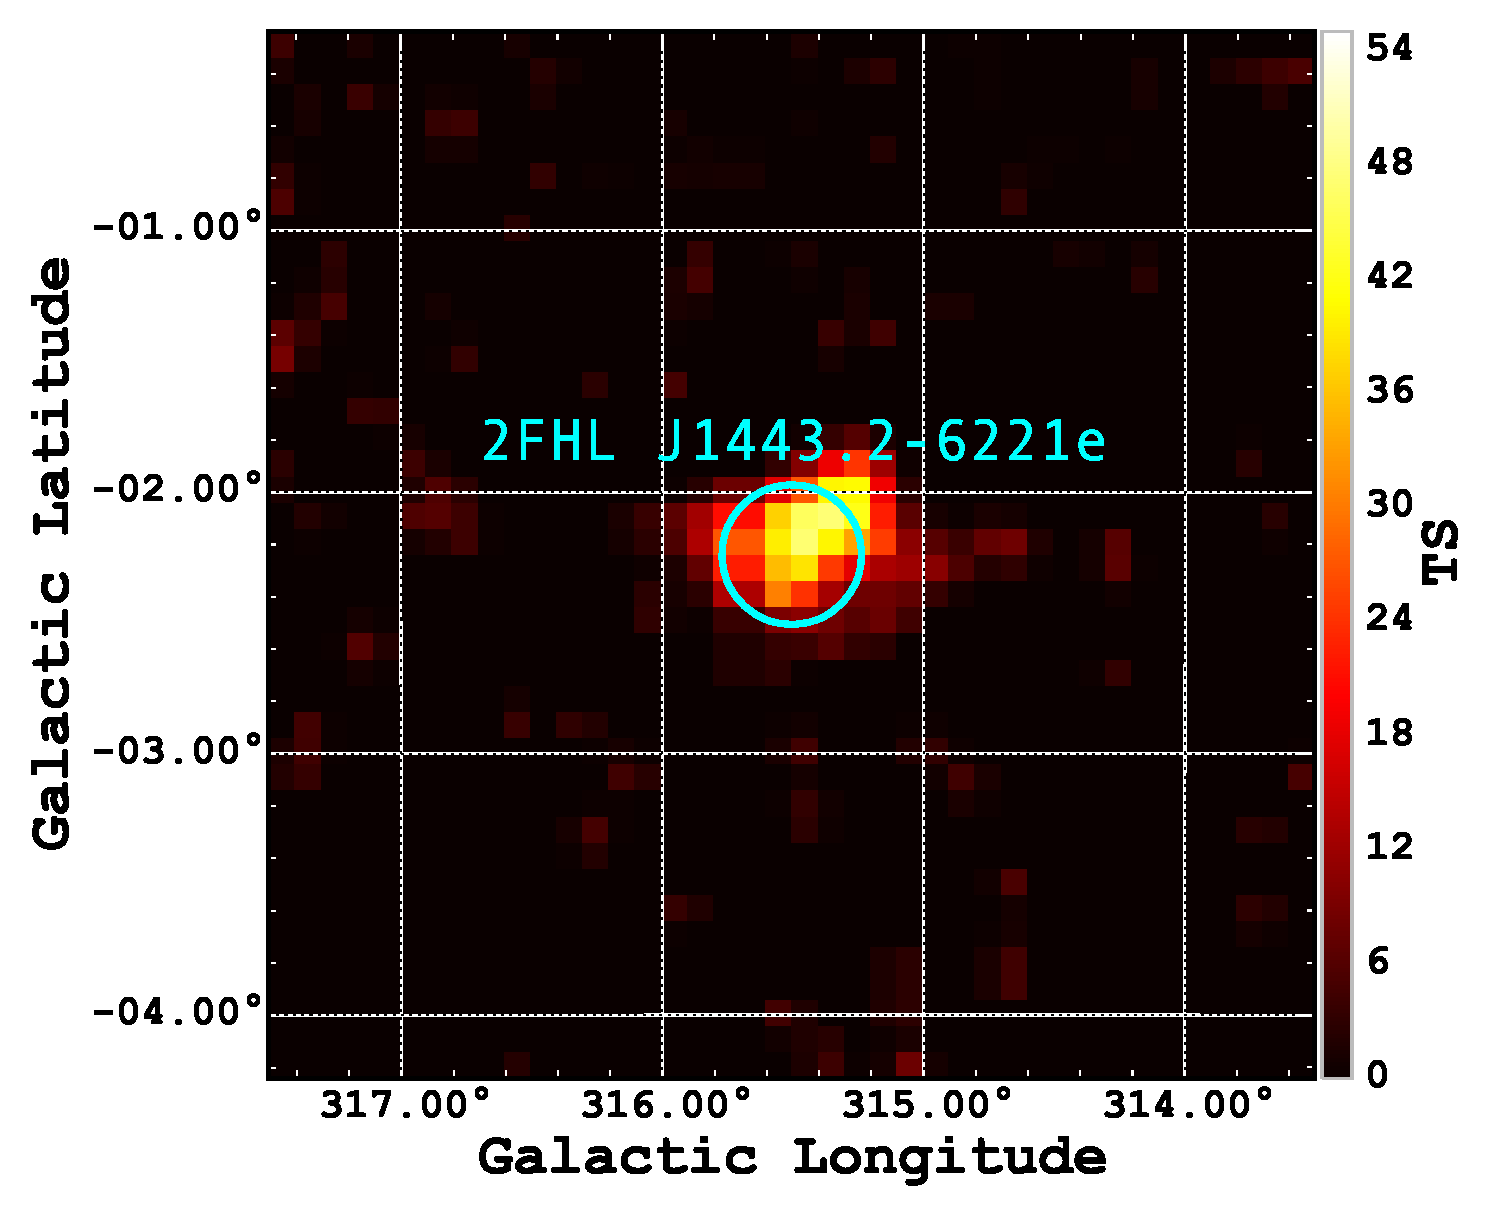
\includegraphics[width=8cm]{Figures/l315_b0_ES_3_residTSmap_2FHL_zoom.eps} &
            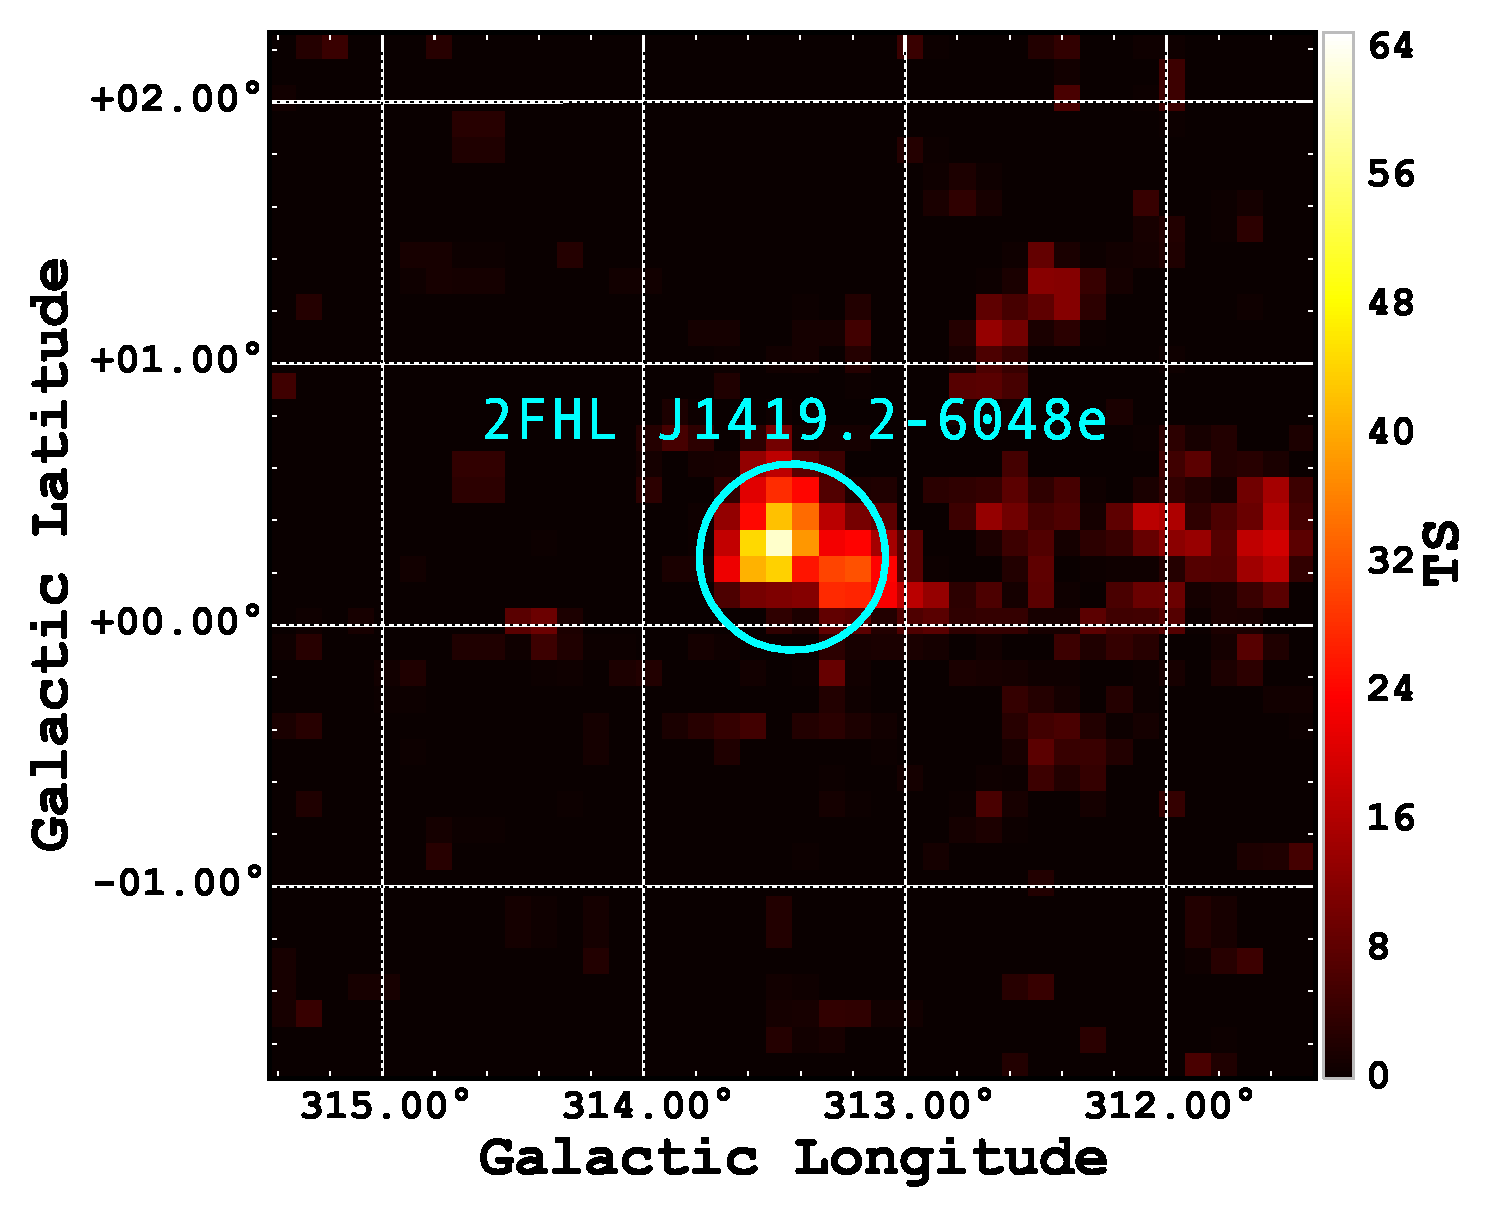
\includegraphics[width=8cm]{Figures/l315_b0_ES_4_residTSmap_2FHL_zoom.eps}\\
            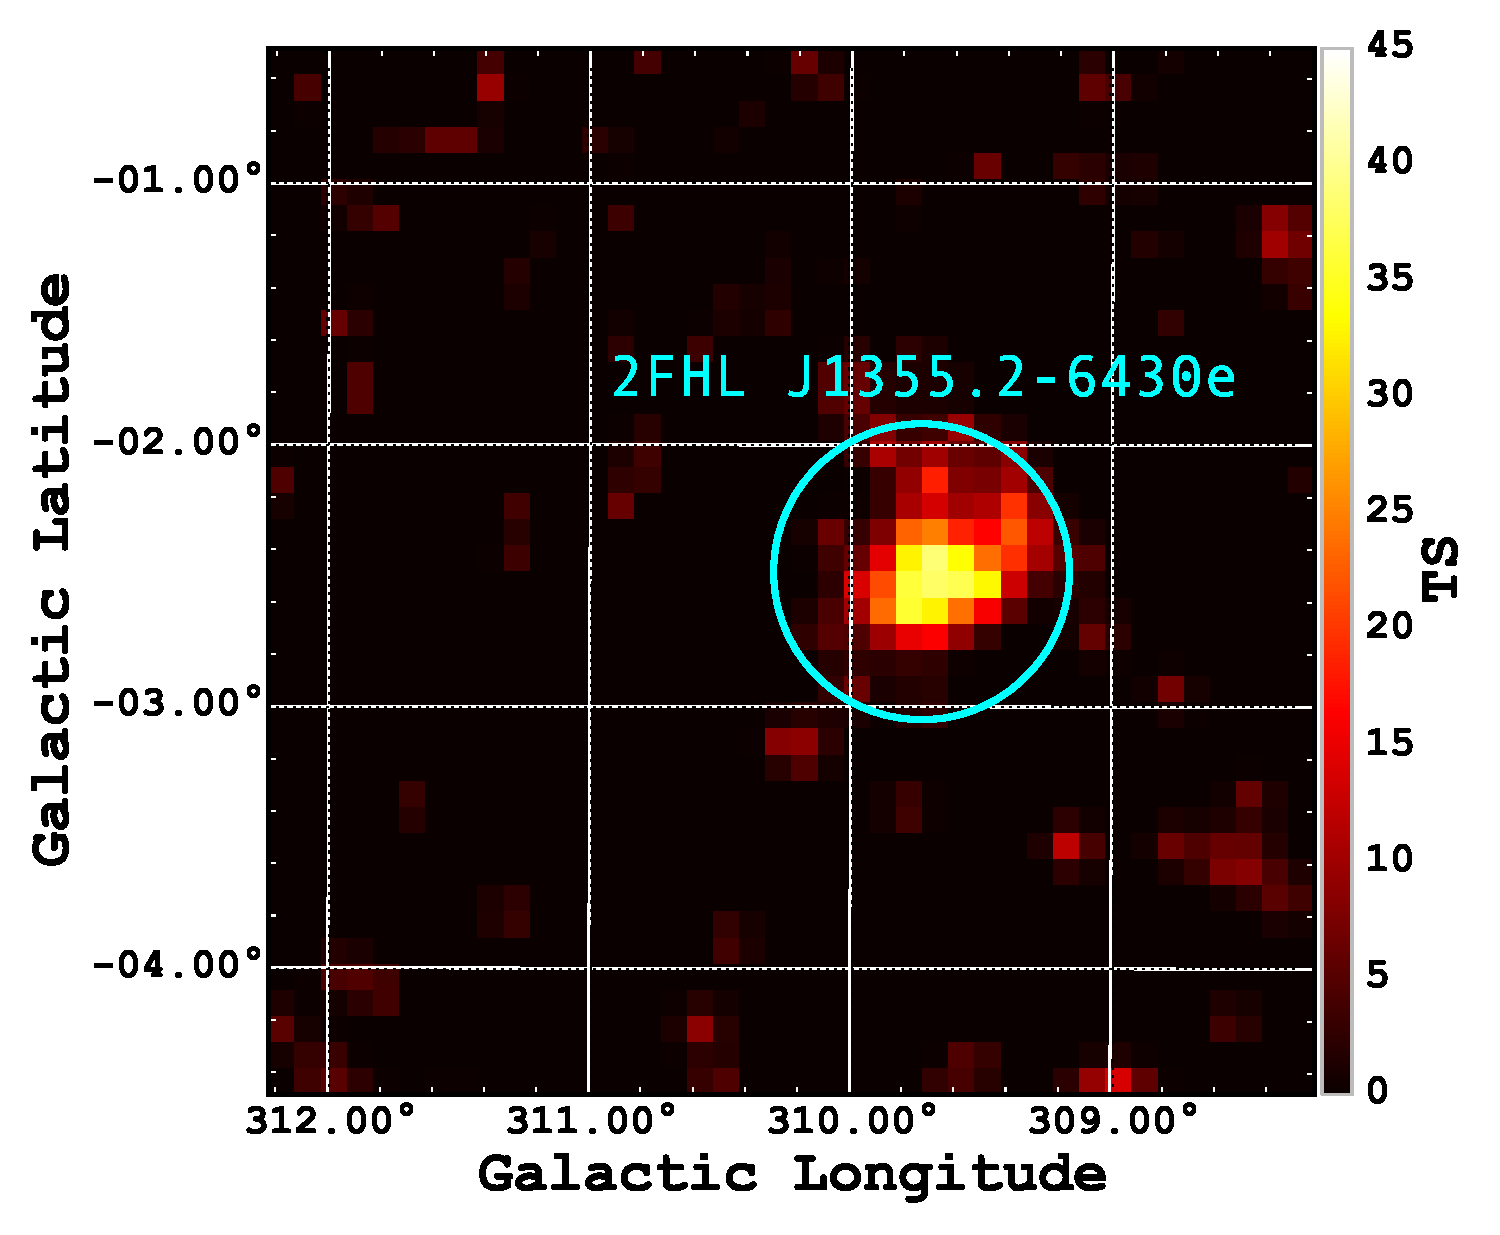
\includegraphics[width=8cm]{Figures/l315_b0_ES_1_residTSmap_2FHL_zoom.eps} &
            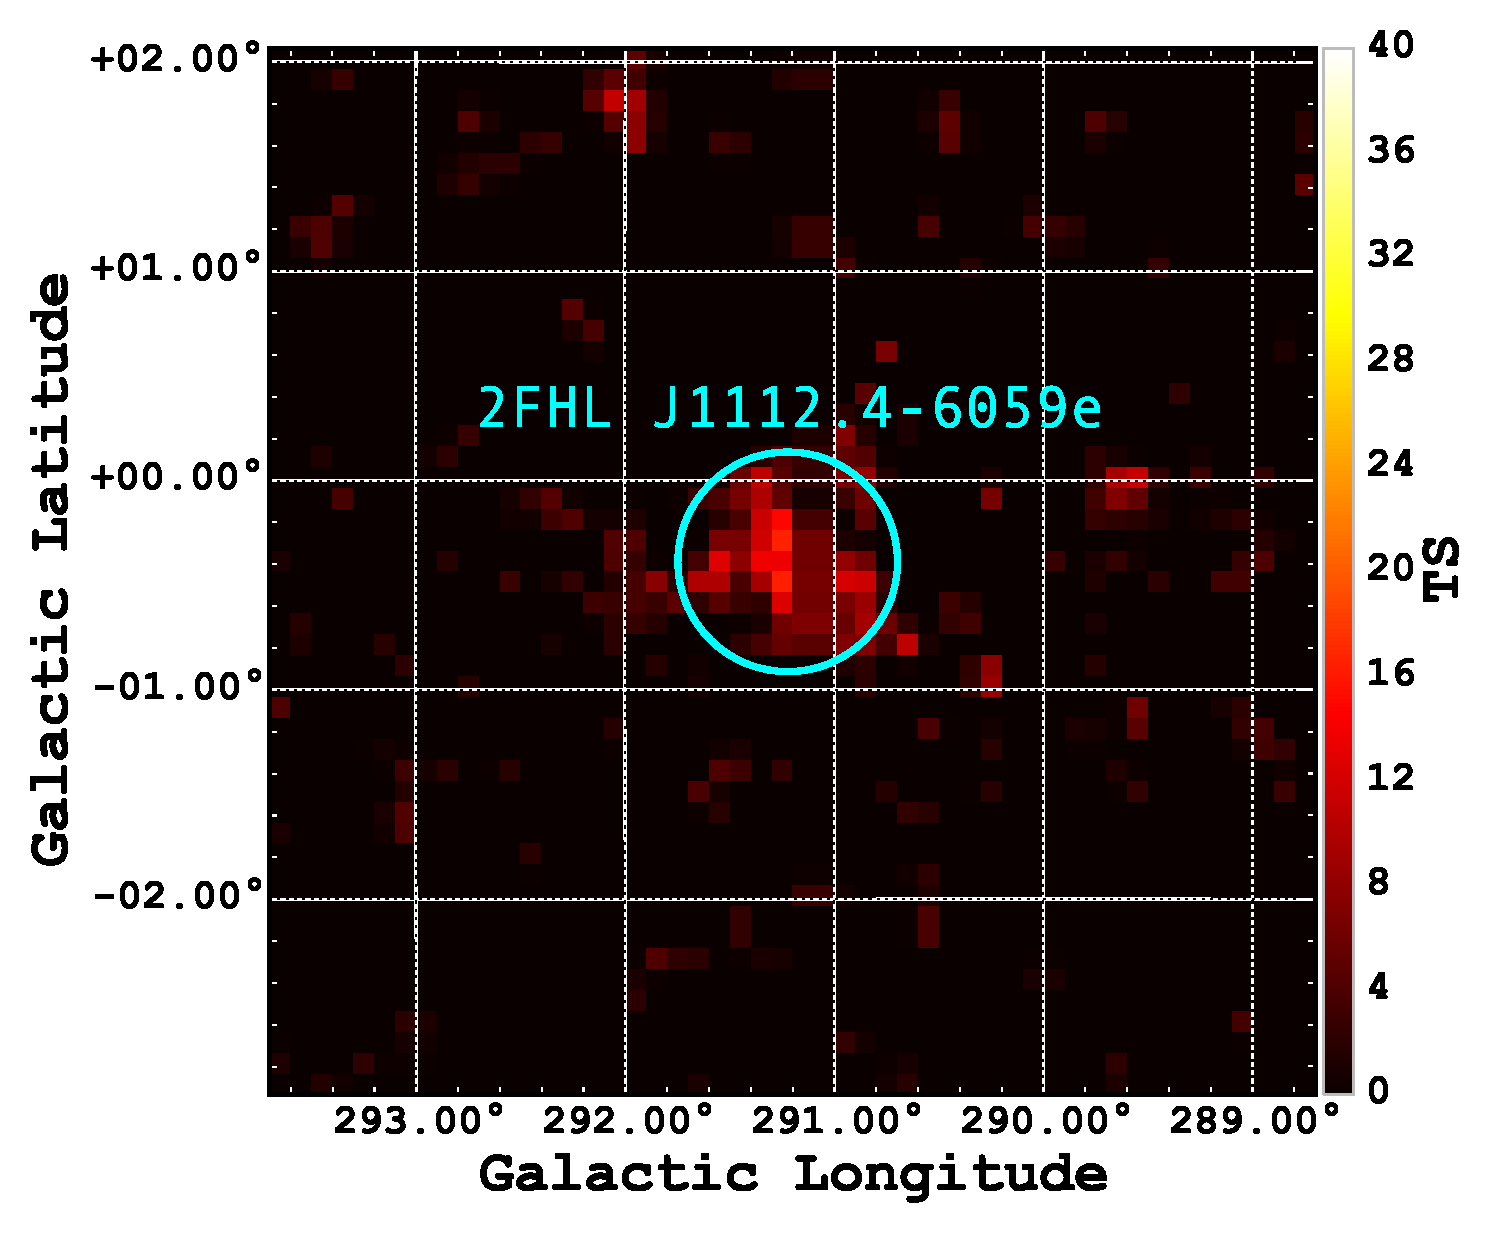
\includegraphics[width=8cm]{Figures/l290_b0_ES_1_residTSmap_2FHL_zoom.eps} \\
            \multicolumn{2}{c}{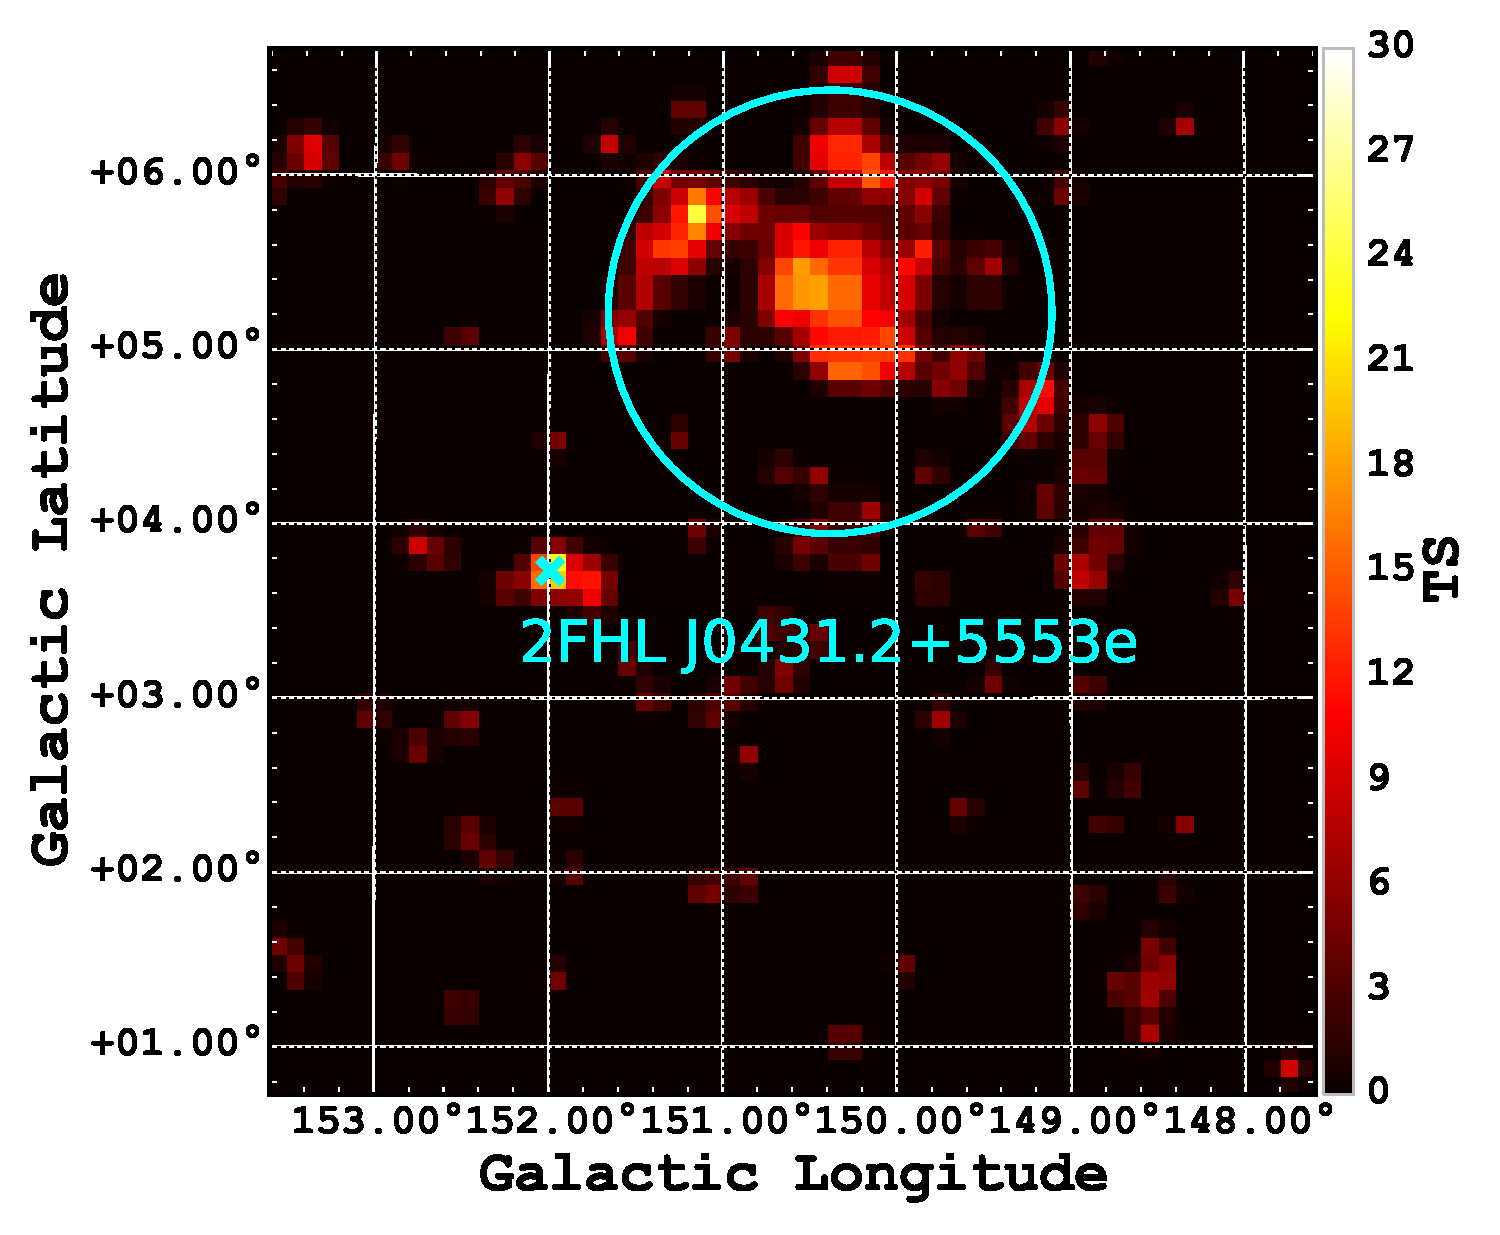
\includegraphics[width=8cm]{Figures/l145_b0_ES_1_residTSmap_2FHL_zoom.eps} }\\
        \end{tabular}
    \end{center}
    \caption{
        \label{fig:6ES} Residual TS maps for the five new extended sources described in Chapter \ref{2fhl:ESresults}.  Only the Galactic diffuse and isotropic emission are included in the model to highlight the location of emission not associated with the diffuse background. Circles indicate the extents of the fit disks. {The x marker in the bottom panel (2FHL~J0431.2+5553e) shows the location of a point source in the \roi{}.}}
\end{figure*}

\begin{deluxetable}{lccclccc}
\setlength{\tabcolsep}{0.04in}
\tablewidth{0pt}
\tabletypesize{\scriptsize}
\tcap{2FHL extended sources previously detected by the {\it Fermi}-LAT \label{tab:extended}}
\tablehead{
\colhead{2FHL Name} & 
\colhead{$l$ [deg]} & 
\colhead{$b$ [deg]} &
\colhead{TS} &
\colhead{Association} &
\colhead{Class} &
\colhead{Spatial model} &
\colhead{Radius [deg]}
}
\startdata
 J0526.6$-$6825e      &    278.843 &    -32.850 & 49.80  & LMC                & gal    & 2D Gaussian 		& 1.87 \\
 J0617.2+2234e        &    189.048 &      3.033 & 398.64 & IC~443             & snr    & 2D Gaussian 		& 0.27 \\
 J0822.6$-$4250e      &    260.317 &	 -3.277 &  63.87 & Puppis A	      & snr    & Disk	     		& 0.37 \\
 J0833.1$-$4511e      &    263.333 &     -3.104 & 49.70  & Vela~X             & pwn    & Disk        		& 0.91 \\
 J0852.8$-$4631e      &    266.491 &     -1.233 & 437.21 & Vela~Jr            & snr    & Disk        		& 1.12 \\
 J1303.4$-$6312e      &    304.235 &     -0.358 & 56.06  & HESS~J1303$-$631   & pwn    & 2D Gaussian 		& 0.24 \\
 J1514.0$-$5915e      &    320.269 &     -1.276 & 165.51 & MSH~15$-$52        & pwn    & Disk        		& 0.25 \\
 J1615.3$-$5146e      &    331.659 &     -0.659 & 128.15 & HESS~J1614$-$518   & spp    & Disk        		& 0.42 \\
 J1616.2$-$5054e      &    332.365 &     -0.131 & 87.18  & HESS~J1616$-$508   & pwn    & Disk        		& 0.32 \\
 J1633.5$-$4746e      &    336.517 &      0.121 & 114.17 & HESS~J1632$-$478   & pwn    & Disk        		& 0.35 \\
 J1713.5$-$3945e      &    347.336 &     -0.473 & 60.98  & RX~J1713.7$-$3946  & snr    & Map         		& 0.56 \\
 J1801.3$-$2326e      &      6.527 &     -0.251 & 50.20  & W~28               & snr    & Disk        		& 0.39 \\
 J1805.6$-$2136e      &      8.606 &     -0.211 & 160.43 & W~30               & snr    & Disk        		& 0.37 \\
 J1824.5$-$1350e      &     17.569 &     -0.452 & 266.09 & HESS~J1825$-$137   & pwn    & 2D Gaussian 		& 0.75 \\
 J1834.9$-$0848e      &     23.216 &     -0.373 &  67.30 & W~41               & spp    & 2D Gaussian		& 0.23 \\
 J1836.5$-$0655e      &     25.081 &      0.136 & 62.72  & HESS~J1837$-$069   & pwn    & Disk        		& 0.33 \\
 J1840.9$-$0532e      &     26.796 &     -0.198 & 163.15 & HESS~J1841$-$055   & pwn    & Elliptical 2D Gaussian & 0.62, 0.38, 39 \\
 J1923.2+1408e        &     49.112 &     -0.466 & 44.60  & W~51C              & snr    & Elliptical Disk        & 0.38, 0.26, 90 \\
 J2021.0+4031e        &     78.241 &      2.197 & 115.97 & Gamma Cygni        & snr    & Disk                   & 0.63 \\
 J2028.6+4110e        &     79.601 &      1.396 & 28.09  & Cygnus Cocoon      & sfr    & 2D Gaussian            & 3.0 \\
\enddata
\tablecomments{~List of the 20 extended sources in 2FHL that were previously detected as extended by the {\it Fermi}-LAT. All these sources are in  3FGL except W41, which is studied by \citet{W41}. The Galactic coordinates $l$ and $b$ are given in degrees. The extension of the disk templates is given by the radius. The extension of the 2D Gaussian templates is given by the $1\sigma$ radius, and the elliptical templates are given by the semi-major axis, semi-minor axis, and position angle (East of North). Association, Class, and Spatial model are as given in \threefgl{}.
}
\end{deluxetable}


\begin{deluxetable}{lcccccccclccc}
\setlength{\tabcolsep}{0.04in}
\tablewidth{0pt}
\tabletypesize{\scriptsize}
\tcap{New 2FHL extended sources 
\label{tab:new_extended}}
\tablehead{
\colhead{2FHL Name} & 
\colhead{$l$ [deg]} & 
\colhead{$b$ [deg]} &
\colhead{TS} & 
\colhead{TS$_{ext}$} &
\colhead{TS$_{2pts}$} &
\colhead{$F_{50}$} & 
\colhead{$\Delta F_{50}$} &
\colhead{$\Gamma$} & 
\colhead{$\Delta \Gamma$} &
\colhead{Association} &
\colhead{Class} &
\colhead{Radius [deg]} 
}
\startdata
 J0431.2+5553e        &    150.384 &      5.216 &  87.9 & 83.4  & 26.2    &  11.70 &       2.11 &    1.66 &         0.20 & G~150.3+4.5     & snr     & 1.27 \\
 J1112.4$-$6059e      &    291.222 &     -0.388 &  80.9 & 68.3   & 22.5    &  12.80 &       2.36 &    2.15 &         0.28 & PSR~J1112$-$6103  & pwn     & 0.53 \\
 J1355.2$-$6430e      &    309.730 &     -2.484 &  82.3 & 31.8   & 12.9     &  9.59  &       1.95 &    1.56 &         0.22 & PSR~J1357$-$6429  & pwn     & 0.57 \\
 %J1407.3$-$6116e      &    311.924 &      0.259 &  68.66 & 30.00       &  14.70 &       2.63 &    2.58 &         0.28 & \nodata         & \nodata & 0.38 \\
 J1419.2$-$6048e      &    313.432 &      0.260 & 109.3 & 49.1   & 15.6    &  17.60 &       2.80 &    1.87 &         0.19 & PSR~J1420$-$6048  & pwn     & 0.36 \\
 J1443.2$-$6221e      &    315.505 &     -2.239 &  75.6 & 29.9   & 19.2   &  7.23  &       1.70 &    2.07 &         0.30 & SNR~G315.4$-$2.3  & snr     & 0.27 \\
\enddata
\tablecomments{~List of the 5 new extended sources in the 2FHL. All these sources are characterized by an uniform disk template whose radius is given in the last column.}
\end{deluxetable}



%%%%%%%%%%%%%%%%%%%%%%%%%%%%%%%%%%%%%%%%%%%%%%%%%%%%%%%%%%%%%%%%
%
%         Summary
%
%%%%%%%%%%%%%%%%%%%%%%%%%%%%%%%%%%%%%%%%%%%%%%%%%%%%%%%%%%%%%%%%
\section{Summary}
\label{sec:summary}

We have presented an all-sky analysis at $\geq$ 50\,GeV
of 80\,months of \lat{} data relying on the new Pass~8 event-level analysis.
Pass~8 delivers improvements in the acceptance and the PSF, reduces
background of misclassified charged particles
and extends the energy range at which the \lat{} is sensitive.
All this allowed the \lat{} to detect 360 sources in the 50\,GeV--2\,TeV range,
performing an unbiased census of the $>$50\,GeV sky for the first time.
%This is the first time that \lat can thoroughly explore this energy range.
This catalog of sources (dubbed 2FHL) provides a bridge between
the traditional 0.1--100\,GeV band of \lat{} catalogs \citep{3FGL}
and the $\gtrsim$100\,GeV band probed by IACTs from the ground.
The 2FHL catalog has the potential to improve the efficiency with
which new sources are detected at TeV energies since only
about 25\,\% of the 2FHL sources were previously detected by IACTs.

%The majority ($\gtrsim$80\,\%)of sources detected in the 2FHL catalog are likely extragalactic because they are either located at high Galactic latitude or are associated with blazars. 

2FHL includes 103 sources in the direction of the Galactic plane ($|b|<10^{\circ}$).
While a fraction of the sources ($\sim$39\,\%) are associated with blazars, the rest
are Galactic and unassociated sources. Galactic sources generally display
much harder photon indices than blazars (median of $\sim$2 versus $\sim$3)
and copious TeV emission, both signs of efficient particle acceleration.
Most Galactic sources are associated with PWNe and SNRs, systems at the end
of the stellar evolution cycle, and are detected as spatially extended.
All the hard (spectral index $<2$) unassociated  sources within the plane
of our Galaxy are likely of Galactic origin, since very few blazars 
have spectra as hard.

The Pass~8 event-level analysis  and accumulated exposure allow the LAT to extend its reach
to higher energy and to open a new window on the sub-TeV sky. Sensitivity improves linearly with time in the photon-limited regime, thus 
further observations by the LAT in the coming years
will probe the $>$\,50\,GeV sky even more deeply, providing
important targets for current and future 
Cherenkov telescopes.

%%%%%%

\chapter{SNR G150.3+4.5}
\label{chap:G150}
Dedicated analysis  of one interesting \twofhl result. First blindly detected extended \g -ray source. 

    -Direct application of addSrcs to an intersting newly detected GeV SNR
    
    -dedicated analysis of the one source to try to understand its nature
    
    -It's interesting because :
    
    -it was blindly detected
    
    -might be the closest rem
    
    -spectrum + index seems like dynamically young, but age and distance are hard to constrain, so it could be older 
    
    -Understanding this remnant contributes to the connection between Fermi and TeV telescopes

Take this all straight from the paper I write. Not sure how much more I'd need to add

\section{Introduction} 
Supernova remnants have long been thought to be the primary accelerators of cosmic rays up to the knee of the cosmic ray energy spectrum. 

what to say about radio SNRs? Connect CRs to nonthermal emission and the LAT and 
Something about SNRs, cosmic ray accelerators, radio detections, connection between radio-LAT observations, G150 detection, 2FHL blind detection and SNRs at TeV (all young?), this paper extends the energy down to

Focus more on the hadronic vs leptonic since that's what's interesting? 
We describe the LAT and analysis results in $\S$\ref{sec:LATobs}, detail multiwavelength observations in $\S$\ref{sec:Multiwave}, and discuss various emission origin scenarios in $\S$\ref{sec:Discuss}.
%%%%%%%%%%%%%%%%%%%%%%%%%%%%%%%%%%%%%%%%%%%%%%%%%%%%%%%%%%%%%%%%
%
%         FermiLat  Observations and  Analysis 
%
%%%%%%%%%%%%%%%%%%%%%%%%%%%%%%%%%%%%%%%%%%%%%%%%%%%%%%%%%%%%%%%%
\section{\label{sec:LATobs}\FermiLat ~Observations and  Analysis }
\subsection{\label{sec:LATdata}Data Set and Reduction}
\FermiLat is a pair conversion telescope sensitive to high energy \gam s  from 20 MeV to greater than 1 TeV \citep{2FHL}, operating primarily in a sky-survey mode which views  the entire sky every 3 hours. The LAT has wide field of view ($\sim$2.4 sr), a large effective area of $\sim$8200 cm$^2$ above 1 GeV for on axis events and a  68\% containment radius angular resolution  of $\sim$0.8$^\circ$  at 1 GeV. For further details  on the instrument and its performance see \cite{atwood09} and \cite{lat_perf}.

In this analysis, we  analyzed 7 years of Pass 8 data, from August 2nd 2008  to August 2nd 2015. The Pass 8 event reconstruction provides a significantly improved angular resolution \jamie{this is sadly unimportant unless I'm at higher energy or using the PSF types. The P8 total PSF at 1 GeV is about the same as for P7REP. It's the acceptance/effective area that are considerably better at this energy}, acceptance, and background event rejection \citep{atwood13b,atwood13}, all of which lead to an increase in the effective energy range and sensitivity of the LAT. Source class events were analyzed within a 14$^\circ$x14$^\circ$ region centered on SNR \Gone~using the P8R2\_SOURCE\_V6 instrument response functions, with a pixel size of 0.1$^{\circ}$. To reduce contamination from earth limb \gam s, only events with zenith angle less than 100$^{\circ}$ were included.

For spectral and spatial analysis we utilized both the standard \Fermi Science Tools (version 10-01-01)\footnote[1]{\url{http://fermi.gsfc.nasa.gov/ssc/}} , and the binned maximum likelihood package \ptlike~\citep{Kerr10}. \ptlike~provides methods for simultaneously fitting the spectrum, position, and spatial extension of a source, and was extensively validated in \cite{Lande12}. Both packages fit a source model, the Galactic diffuse emission, and an isotropic component (which accounts for the background of misclassified charged particles and the extragalactic diffuse \gam~ background)\footnote[2]{\url{http://fermi.gsfc.nasa.gov/ssc/data/access/lat/BackgroundModels.html}} to the observations. In this analysis, we used the standard Galactic diffuse ring-hybrid model scaled for Pass 8 analysis, gll{\_}iem{\_}v06.fits (modulated by a power law function with free index and normalization), and for the isotropic emission,  we used iso{\_}P8R2{\_}SOURCE{\_}V6{\_}v06.txt, extrapolated to 2 TeV as in \cite{2FHL}.

In our source model for the region, we included sources from the third \FermiLat catalog \citep[3FGL]{3FGL} within 15$^\circ$ of the center of our region of interest (RoI). We replaced the position and spectrum of any 3FGL pulsars in the region with their corresponding counterpart  from the LAT 2nd pulsar catalog \citep{2PC}.  Residual emission unaccounted for by 3FGL sources is present in the RoI due to the increased time range and different energy selection with respect to that in 3FGL. We added to the RoI several point sources to account for this unmodeled emission and minimize the global residuals.\jamie{do I need to say more about these sources? should I mention adding them automatially and iteraively based on TS maps and reference SNRcat/2FHL? How close is the closest source? Mention this and use as an argument for not saying much more about them}.  The normalization and spectral index of sources within 5$^{\circ}$ of the center of the RoI were free to vary, whereas all other source parameters were fixed. A preliminary maximum likelihood fit of the RoI was performed, and  sources with a test statistic (TS) $<$ 9 (TS is defined as,  ${\rm TS}=2~{\rm Log}(\mathcal{L}_1 / \mathcal{L}_0)$ where $\mathcal{L}_1$ 
is the likelihood of source plus background and  $\mathcal{L}_0$ that of just the background) were removed from the model. 

\subsection{\label{sec:LATmorph}Morphological Analysis}
Studying the spatial extension of sources with the LAT is non-trivial due to the energy-dependent point spread function (PSF) and strong diffuse emission present in the Galactic plane. Soft spectrum point sources and uncertainties in the diffuse model can be a source of systematic error when not accurately modeling extended emission as such, particularly at low energies where the PSF is broad. To strike a balance between the best angular resolution and minimal source and diffuse contamination, we restrict our morphological analysis to energies between 1 GeV and 1 TeV. We divide this energy range into 12\jamie{4bpd} logarithmically spaced bins for both \ptlike~and \gtlike~binned likelihood analyses. 

Three  unidentified 3FGL sources are located within the extent of \Gone. 3FGL J0425.8+ 5600, located approximately 0.6$^\circ$ from the center of the SNR, is the closest of the three sources and is described with a power law spectrum of index ${\rm \Gamma = 2.35\pm 0.17}$  in the 3FGL catalog. The closest radio source to 3FGL J0425.8+5600 is NVSS J042719+560823, at 0.25° away (Ref?). 3FGL J0423.5+5442, exhibits a power law spectral index, ${\rm \Gamma = 2.63\pm 0.15}$, with no clear multiwavelength source association. Finally, 3FGL J0426.7+5437 has a pulsar-like spectrum, yet in a timing survey performed with the 100-m  Effelsberg radio telescope, \cite{Barr13} were unable to detect pulsations from the source down to a limiting flux density of $\sim$ 0.1 mJy. The source is located about 0.8$^{\circ}$ from the center of the SNR. We discuss this source and potential association with \Gone ~further in $\S$\ref{sec:Dist}). 

In our analysis, we removed 3FGL J0425.8+5600 and 3FGL J0423.5+544 from the RoI, but kept 3FGL J0426.7+5437 in the model since preliminary analyses showed clear positive residual emission at the position of the source if it was removed from the RoI. Figure \ref{fig:1GeV_resTSmap} shows a residual TS map for the region around \Gone. This point source detection-significance map was created by placing a point source modeled with a power law of photon index, $\Gamma$ = 2 at each pixel and gives the significance of detecting a point source at each location above the background. 

%put file name in {} to get it to compile with dots in the name!
%for png, have to use pdfchain
\begin{figure}[!ht]
	\begin{centering}
		\includegraphics[width=\columnwidth]{{Figures/G150_1GeV_resTsmap_radio_noLabs}.pdf}
		\caption{Background subtracted residual TS map above 1 GeV with 0.1$^\circ$x 0.1$^\circ$ pixels for fixed index $\Gamma$ = 2, centered on SNR \Gone. The orange circle and translucent shading show the fit disk radius and 1$\sigma$ errors, respectively, for the extended source, the orange cross shows the position of 3FGL J0426.7+5437 (included in the background model), and blue dashed circle is the extent of the radio SNR. 
			\label{fig:1GeV_resTSmap}}
	\end{centering}
\end{figure}

\begin{figure}[!ht]
	\begin{centering}
		\includegraphics[width=\columnwidth]{{Figures/G150_1GeV_resTsmapNoG150_radio_noLabs}.pdf}
		\caption{Same as Figure \ref{fig:1GeV_resTSmap} but with disk in the background model \jamie{should this be a residual counts map instead?}
			\label{fig:1GeV_resTSmap_noG150}}
	\end{centering}
\end{figure}

%\begin{figure}[!ht]
%	\begin{centering}
%		\includegraphics[width=\columnwidth]{Figures/G150_GaoHan.png}
%		\caption{This is just a filler image for now while testing things out \citep{Gao14}
%			\label{fig:GaoRad}}
%	\end{centering}
%\end{figure}

We modeled the excess emission in the direction of \Gone ~with a uniform intensity, radially-symmetric disk, simultaneously fitting the spatial and spectral components of the model  via \ptlike. The extension of the disk was initialized with a seed radius of $\sigma$ = 0.1$^\circ$ and position centered on the radio position of \Gone. We define the significance of extension as in \cite{Lande12}; ${\rm TS_{ext} = 2~log(\mathcal{L}_{ext} / \mathcal{L}_{ps})}$, with $\mathcal{L}_{ext}$ being the likelihood of the model with the extended source and $\mathcal{L}_{ps}$ that with of a point source located at the peak of emission interior to the extended source. For the disk model,  ${\rm TS_{ext} = 298}$, with a best fit radius, ${\rm \sigma = 1.40^\circ \pm 0.03^\circ}$ \jamie{I should just put this all in a table and reference it}, which is in excellent agreement with the radio size of the SNR determined in \cite{Gao14}. We tried adding back in to our model the two removed 3FGL sources but both were insignificant when fit on top of the best fit disk. Figure \ref{fig:1GeV_resTSmap_noG150} is a Residual TS map of the same region as Figure \ref{fig:1GeV_resTSmap}, but with the disk source included in the background showing that the disk can account well for the emission in the region. 

The morphology of the radio emission is suggestive of an elliptical or ring morphology, so an elliptical disk and ring spatial model were tested as well. For the ring model, the fit reduced to a disk with parameters matching those stated above. Using the elliptical model showed a weak improvement over the radially symmetric model at the 2.6$\sigma$ level (${\rm \Delta TS = 9}$ with two additional degrees of freedom), which we did not consider significant enough to say the GeV emission had an elliptical morphology (see Table \ref{tab:LATres}). For the remainder of this study, we only considered the disk spatial model.\jamie{put Edisk in table too and reference i.}
\jamie{I should double check this for 1GeV- 1TeV. I was done for 1-562 GeV, wait till addSrcs is done}



Other things we tried

fitting an extended source (starting with the 2FHL result) on top of the one currently there. Insignif. idk what to say about 2FHL yet. 

another starting at the position of G149. Insignif


Say something about why we don't just go with the 3 3FGL sources. In the table I shouldn't just compare the 3 to the disk though because I also keep J0426 in the model. So the base comparison is really 2 sources vs the disk. Maybe it's enough to just say of course we keep the disk, we find one at GeV that matches really well with the radio. What did Josh's paper say about how modelling the spectrum of an intrisically extended source as point sources skews the PS spectrum to softer energies?

He said, "Specifically, modeling a spatially extended source as point-like will systematically soften measured spectra", but idk if I get why. We see it with the 2 3FGL sources being softer than what the disk winds up being

Another thing to point out is how modeling as point vs extended, if it's really extended can affect the fit of other point sources nearby, like J0426, so I should show the spectrum of this source too?  I fit both the norm and index of the source. 
\begin{deluxetable}{cccccccc}
\setlength{\tabcolsep}{0.04in}
\tablewidth{0pt}
\tabletypesize{\scriptsize}
\tablecaption{LAT Analysis Results\label{tab:LATres}}
\tablehead{
\colhead{Spatial Model\,\tablenotemark{a}} & 
\colhead{TS} & 
\colhead{TS$_{ext}$} &
\colhead{$\sigma$} &
\colhead{Association} &
\colhead{Class} &
\colhead{Spatial model} &
\colhead{Extension [deg]} \\
\colhead{} & 
\colhead{} & 
\colhead{} &
\colhead{$^\circ$} &
\colhead{} &
\colhead{} &
\colhead{} &
\colhead{}}
\startdata
J0526.6$-$6825e      &    278.843 &    -32.850 & 49.80  & LMC                & gal    & 2D Gaussian         & 1.87 \\
J0617.2+2234e        &    189.048 &      3.033 & 398.64 & IC~443             & snr    & 2D Gaussian         & 0.27 \\
J0822.6$-$4250e      &    260.317 &  -3.277 &  63.87 & Puppis A       & snr    & ...               & 0.37 \\
%\cutinhead{Thee Point Sources}
%\sidehead{Uniform Disk}

\enddata
\tablecomments{~This is mostly from 2FHL, just playing with the table. Don't need a table for just disk hypothesis, but maybe to have disk 3  point sources compatison. I tried adding more sources on top of the 3FGL sources and there's no significant residual. where to say something about testing searching for point sources overlapping the extended source and trying to fit an extended source on top as well? in this table give the disk model with best spectral spatial params, TS, TSext  dof, LL, then the model with just the 3 3FGL sources (no disk) spectrum of each, TS, dof + LL( didn't relocalize the se sources), separate spatial spectral tables?
}
\tablenotetext{a}{comments and notes?}
\end{deluxetable}



\subsection{\label{sec:LATspec}Spectral Analysis}
After determining the best fit morphology with \ptlike~for the GeV emission coincident with SNR \Gone, we used those results as a starting point for our \gtlike~maximum likelihood fit of the region to estimate the best spectral parameters for our model. The LAT data is well described by a power law across the entire energy range with a photon index, ${\rm \Gamma = 1.80 \pm 0.04}$, and energy flux above 1 GeV of ${\rm (7.17 \pm 0.73~ x 10^{-11})~ erg~cm^{-2}~ s^{-1}}$and TS = 373 \jamie{these are the pointlike results, change them when I get the gtlike res}. We tested the \gam ~spectrum of the extended disk for spectral curvature using a log-normal model (Log Parabola), and find no significant deviation from a power law (${\rm \Delta TS \sim 1}$). 

\begin{figure}[!ht]
	\begin{centering}
		\includegraphics[width=\columnwidth]{Figures/{G150.3+4.5_SED}.png}
		\caption{Spectral energy distribution for the extended source coincident with SNR \Gone. \jamie{replace with gtlike SED when I have it}
			\label{fig:G150SED}}
	\end{centering}
\end{figure}

\begin{figure}[!ht]
	\begin{centering}
		\includegraphics[width=\columnwidth]{Figures/{G150.3+4.5_3FGLJ0426.7+5437_SED}.png}
		\caption{Spectral energy distribution of 3FGL J0426.. \jamie{replace with gtlike SED when I have it}
			\label{fig:J0426SED}}
	\end{centering}
\end{figure}
Still to do

gtlike


Systematics. Bracketing IRFs, alt iem, try varying the extension? still need to be done. Should probably just move this into the spectral  section


%%%%%%%%%%%%%%%%%%%%%%%%%%%%%%%%%%%%%%%%%%%%%%%%%%%%%%%%%%%%%%%%
%
%         Multiwavelength  Observations and  Analysis 
%
%%%%%%%%%%%%%%%%%%%%%%%%%%%%%%%%%%%%%%%%%%%%%%%%%%%%%%%%%%%%%%%%

\section{\label{sec:Multiwave}Multiwavelength  Observations and  Analysis }
\subsection{\label{sec:HI}HI}
\subsection{\label{sec:CO}CO?}
Do the CO maps add anything?
\subsection{\label{sec:Xray}X-ray}
No diffuse nonthermal X-ray emission observed by ROSAT. No point sources near the center? Should a  pulsar even  be near the center? How to quantify this? Can we place a limit on ambient density with an upper limit on thermal X-ray emission? Magnetic filed with nonthermal?

%%%%%%%%%%%%%%%%%%%%%%%%%%%%%%%%%%%%%%%%%%%%%%%%%%%%%%%%%%%%%%%%
%
%         Discussion and Results
%
%%%%%%%%%%%%%%%%%%%%%%%%%%%%%%%%%%%%%%%%%%%%%%%%%%%%%%%%%%%%%%%%
\section{\label{sec:Discuss}Discussion and Results}
\subsection{\label{sec:What}What is it?}
Size + HI suggest that near distance corresponding to different HI velocities suggest it's aged, spectrum looks more like young SNR (hard + no GeV break ). Is it a weird young remnant or weird aged one? Leptonic dominated if young, hadronic dominated if older? Something about nearby dense clouds masking hadronic emission? Maybe this is only true for MeV cosmic rays that are screened out though and it would only mask the pion bump, but not this higher energy emission?

PWN or SNR. Can we rule out PWN? See W41 paper, MSH 11-61A, Fabios recent G326 work (no, he just tries to use the PSF types and testing different model templates to try to disentangle SNR from PWN)?

No PSR candidate near center (should it be near the center? Depends on age)
Is there some limit we can place on the PWN based on not seeing the pulsar? Like on Edot? OR something like Mattana et al. 2009 correlation between  $\mathrm{flux_x / flux_g \propto}$   Edot? 

Assume it's in Sedov phase based on size + near distance, and calculate age, upper limit on Edot base on lack of x-ray flux? Or maybe if I assume the sources is the PWN and GeV radius is PWN radius, then can I estimate Edot based on size and evolution inside  SNR?

If we assume close distance, age is only $\approx$ 5kyr, maybe this is a transitional SNR? What do others like this look like? Puppis A? Gamma Cygni is a similar age too.something 


\subsection{\label{sec:Dist}Distance Considerations}
probably doesn't need to be a different section. 
\subsection{\label{secModel}Nonthermal Modeling}
I think I could get a working model with naima running pretty quickly, is it worth it?
%%%%%%%%%%%%%%%%%%%%%%%%%%%%%%%%%%%%%%%%%%%%%%%%%%%%%%%%%%%%%%%%
%
%         Conclusion
%
%%%%%%%%%%%%%%%%%%%%%%%%%%%%%%%%%%%%%%%%%%%%%%%%%%%%%%%%%%%%%%%%
\section{\label{sec:Conc}Conclusions}
\jamie{most of this should be the conclusions from the G150 paper}In this chapter, we have presented the publication on the dedicated analysis of the extended \g -ray emission detected in the direction of \Gone. \Gone ~was first detected in radio by \cite{Gao14}, and subsequently detected in \g-rays in \twofhl above 50 \gev. We discussed our \lat morphological analysis at energies E $\geq$ x \gev~and spectral analysis down to E $\geq$ 750 \mev, demonstrating a change in extension and centroid position compared to the \twofhl result. Discuss potential source origin scenarios. Is it SNR or PWN? Is \twofhl source same as $>$ few \gev? 

\jamie{for diss, not paper}. The way this figures into the whole is that  this is a follow up analysis of one of the most interesting  sources detected with addSrcs, and, (hopefully!), we're able to say something about the source and nature of the \g-ray emission, relation to SNR and \twofhl source1
\chapter{SNR-MC, 10 GeV, and anything else?}
\label{chap:other}

Not sure how this is going to factor in yet. SNR-MC should fit in somehow since a good deal of work was done? Less certain about 10gev. 
\chapter{Conclusions}\label{chap:conc}
In this dissertation we investigated the \gam{} emission from \snrs{} to obtain a better understanding of the origin of Galactic \crs{}. We performed both individual and population studies of the nonthermal, high-energy, radiation from \snrs{} as a means of probing the underlying \cray{} particle population. The advent of the \lat{}, onboard the \Fermi{} Gamma-Ray Space Telescope, has proved a great boon to studying the \snr{}/\cray{} connection. The \lat{}'s excellent spatial and spectral resolution combined with its wide field of view and survey mode operation has provided for the first time the opportunity to study the \gam{} morphology of \snrs{} as well as probe the hadronic and leptonic \cray{} acceleration processes generating \gam{} photons.

One part of this thesis consisted of the development of an automated analysis method, rooted in a maximum-likelihood framework, to systematically detect and add statistically significant \gam{}-ray sources to an \roi{}. Applying this method, we performed for the first time a characterization of the\gev{} emission around all radio observed \snrs{} with the goal of uniformly cataloging the global properties of this \gam{} emitting population. This analysis allowed us to classify 30 sources as likely\gev{}  \snrs{} and we found that previously adequate, simple \cray{} acceleration models can not sufficiently describe the spectral properties of many \lat{} observed \snrs{}. 

Next, we conducted a survey of the \gam{} sky between 50\gev{} and 2\tev{}, making use of the recent pass 8 event reconstruction analysis. This work served to bridge the energy gap between previous \lat{} 1-100}\gev{} catalog observations and those of ground-based, Cherenkov telescopes with operating energies extending to the sub-TeV regime. A total of 360 sources were detected across the entire sky, with only 25\% previously detected by \iacts{}, demonstrating that this catalog can serve to improve the efficiency of\tev{} source detection and act as pathfinder for future \iact{} observations. The work presented in this dissertation focused on the Galactic results of the catalog, with 11\% of sources being associated with known Galactic objects (primarily \snrs{} and \pwne{}), and 13\% having no known multiwavelength counterpart. We showed that the Galactic objects display significantly harder spectra than extragalactic sources, suggesting that many of the unidentified sources are likely of a Galactic origin. 31 sources were detected as spatially-extended. 4 of these were previously detected but unresolved by the \lat{}, and one, partially overlapping SNR \Gone{}, was the first blindly-detected extended \lat{} source. 

The final study presented here is a follow-up analysis of the \gam{} emission coincident with SNR \Gone{} aimed at understanding the origin of the extended \gam{} source and its connection to the radio \snr{}. Lowering the analysis energy range down to 1\gev{}, we detected significantly extended,  hard \gam{} emission with a morphology in excellent agreement with the large, radio observed \snr{}. We employed archival HI and X-ray data to estimate the distance to \Gone{}  and constrain the ambient density in the vicinity of the remnant. Combining our\gev{} results the with these environmental constraints, we determined that the \snr{} is between 500  and a few thousand years old, likely placing \Gone{} in the dynamically young stage of evolution \ie{} not yet interacting with surrounding molecular material. Supporting this statement, we also determined that the spectral properties and under-luminous power emitted by the \snr{} in \gam{}s is inconsistent with an evolved \snr{} whose shock has encountered nearby molecular clouds. 

In closing, these studies demonstrate the ongoing potential of the \lat{} to reveal and fill in the gaps in the faint radio and \gam{} emitting \snr{} population, particularly in the higher energy, signal-dominated (\ie{} sensitivity improves linearly with time) regime. The work performed in this dissertation, along with future \lat{} \snr{} studies will be of tantamount importance for the up and coming class of ground-based Cherenkov telescopes. Follow-up pointed observations of the  catalog sources, first detected and presented in this dissertation, with\tev{} telescopes (\veritas{}, \hess{}, and the forthcoming Cherenkov Telescope Array) will be able to resolve structure on a finer scale, allowing for refined analysis of the \gam{} emission mechanisms acting at \snr{} shock fronts. \hawc{} observatory, with it's wide field of view, and \textit{}overhead sky-survey method will complement the study of the sources detected in this thesis, with both an overlapping energy range and the capability to detect broadly extended sources. Leveraging the \lat{}'s unique capabilities in tandem with broadband observations of \snrs{} will aid in uncovering and resolving these \gam{} sources which is vital to assessing the ability of \snrs{} to account for the total power in \crs{} in our Galaxy, and to determine if \snrs{} can truly accelerate particles to the knee of the \cray{} energy spectrum. 






%%List of abbreviations
%\newaonym[longplural={Frames per Second}]{fpsLabel}{FPS}{Frame per Second}

%\newacronym{LAT}{name = {LAT}, text ={lare area telescope}, description ={ Large Area Telescope}}%simple example
%\newglossaryentry{uppercase}{
%	name={Uppercase},
%	text={uppercase},
%	description={Appears uppercase in the glossary and lowercase in the text}
%}

\newacronym{onefgl}{1FGL}{First \emph{Fermi}-LAT source catalog}
\newacronym{twofgl}{2FGL}{Second \emph{Fermi}-LAT source catalog}
\newacronym{threefgl}{3FGL}{Third \emph{Fermi}-LAT source catalog}
\newacronym{onefhl}{1FHL}{First Catalog of Hard \emph{Fermi}-LAT Sources}
\newacronym{twofhl}{2FHL}{Second Catalog of Hard \emph{Fermi}-LAT Sources}
\newacronym{twopc}{2PC}{Second \emph{Fermi}-LAT catalog of Gamma-ray Pulsars}
\newacronym{acd}{ACD}{anti-coincidence detector}
\newacronym{agn}{AGN}{active galactic nuclei}
\newacronym{bpl}{BPL}{broken power law}
\newacronym{calo}{CAL}{Calorimeter}
\newacronym{cmb}{CMB}{Cosmic Microwave Background}
\newacronym{cgro}{CGRO}{Compton Gamma-Ray Observatory}
\newacronym[plural=CRs]{cr}{CR}{cosmic ray}
\newacronym{cta}{CTA}{Cherenkov Telescope Array}
\newacronym{dsa}{DSA}{diffusive shock acceleration}
\newacronym{dm}{DM}{dispersion measure}
\newacronym{ecpl}{ECPL}{exponentially cut-off power law}
\newacronym{egret}{EGRET}{Energetic Gamma-Ray Experiment Telescope}
\newacronym{fov}{FoV}{field of view}
\newacronym{fir}{FIR}{far infrared}
\newacronym{gbm}{GBM}{Gamma-Ray Burst Monitor}
\newacronym{grb}{GRB}{gamma-ray burst}
\newacronym{he}{HE}{high energy}
\newacronym{hep}{HEP}{highest-energy photon}
\newacronym{hess}{H.E.S.S.}{the High Energy Stereoscopic System}
\newacronym{ic}{IC}{inverse Compton}
\newacronym{iem}{IEM}{interstellar emission model}
\newacronym{irf}{IRFs}{instrument response functions}
\newacronym[plural=IACTs]{iact}{IACT}{Imaging Air Cherenkov Telescopes}
\newacronym{ism}{ISM}{interstellar medium}
\newacronym{lat}{LAT}{Large Area Telescope}
\newacronym{lrt}{LRT}{likelihood ratio test}
\newacronym{magic}{MAGIC}{the Major Atmospheric Gamma-ray Imaging Cherenkov telescopes}
\newacronym[plural =MCs]{mc}{MC}{molecular cloud}
\newacronym{msp}{MSP}{millisecond pulsar}
\newacronym{nir}{NIR}{near infrared}
\newacronym{ns}{NS}{neutron star}
\newacronym{pl}{PL}{power law}
\newacronym{psf}{PSF}{point spread function}
\newacronym[plural=PSRs ]{psr}{PSR}{pulsar}
\newacronym[plural=PWNe ]{pwn}{PWN}{pulsar wind nebula}
\newacronym[plural=RoIs ]{roi}{RoI}{region of interest}
\newacronym[plural=SEDs]{sed}{SED}{spectral energy distribution}
\newacronym{sedt}{ST}{Sedov-Taylor}
\newacronym[plural=SNRs ]{snr}{SNR}{supernova remnant}
\newacronym{tkr}{TKR}{tracker}
\newacronym{ts}{TS}{test statistic}
\newacronym{veritas}{VERITAS}{the Very Energetic Radiation Imaging Telescope Array System}
\newacronym{vhe}{VHE}{very high energy}
\newacronym{snrmc}{SNR-MC}{supernova remant molecular cloud system}



%So I don't have to type gls all the time

%List of Symbols

\newglossaryentry{nh}
{
	name={\ensuremath{~\mathrm{N_{\rm{H}}}}},
	description={Neutral Hydrogen Number Density},
	sort=Nh
}


% APPENDICES --- Note: only use the \appendix command once before the
%                      first appendix
%%\appendix
%%input{appendix.tex}
%\acrodef{WWW}{World Wide Web}


% Make Glossary
\printglossaries
%\printglossary

% BIBLIOGRAPHY
\phantomsection
\cleardoublepage %Jame added this to get  bib page # in toc corect with glossary included
\addcontentsline{toc}{chapter}{Bibliography}
\bibliographystyle{bst/apj}
%\bibliographystyle{bst/astroadswithlinks} %jam added this from mmks, but it doesn't get the bib right
%This one give full titles for papers.
%\bibliographystyle{apalike}
%\bibliography{thesis-refs}
\bibliography{bib/biblio}
%\bibliography{snrCat}
%%%%%%%%%%%%%%%%%%%%%%%%%%%%%%%%%%%%%%%%%%%%%%%%%%%%%%%%%%%%%%%%%%%%%%%%%%%

\end{document}
